\section{気体の状態変化と熱機関}

% ===========================================================================
%  再編（2026-09-21）：第3章 熱力学 の第23回（熱力学の最終回）．
%  原本の 第16回「気体の状態変化(1)」の 16.2（気体が外界に対してする仕事）と，
%  第17回「気体の状態変化(2)」の全体（等温・断熱・自由膨張），および
%  第18回「熱力学総合演習」の 18.1（熱機関）を合流させて1回とした．
%    `saihen/再編案.md`「新23 ＝ ⑯[17][18][21][22] ＋ ⑰[24]〜[30] ＋ ⑱[31][32]（A2→1）」の通り．
%
%  ・練習は12題（A問題2題を1題に統合）．講義の節順に並べ替えた．
%      ［22］＝ ⑯[17]＋⑰[24]（A問題の統合。定圧の仕事／第一法則／比熱比）
%      ［23］＝ ⑯[18]（$p$-$V$図から仕事を読む）      ［24］＝ ⑯[22]（鉛直シリンダー・定圧）
%      ［25］＝ ⑯[21]（等温変化の仕事）              ［26］＝ ⑰[26]（定温変化）
%      ［27］＝ ⑰[27]（断熱変化）                    ［28］＝ ⑰[28]（断熱自由膨張）
%      ［29］＝ ⑰[29]（断熱膨張・断熱自由膨張）      ［30］＝ ⑰[25]（各物理量の変化のまとめ）
%      ［31］＝ ⑱[31]（サイクル）                    ［32］＝ ⑱[32]（サイクル）
%      C問題 ［33］＝ ⑰[30]（気体の一般的な状態変化）
%    原本は ⑰[25]〈状態変化に伴う各物理量の変化〉をB問題の先頭に置いていたが，
%    設問(4)が断熱変化なので断熱の後ろへ移し，4つの状態変化のまとめとして
%    サイクルの直前に置いた．
%    ⑱[31][32] は `physics_ch18.tex` がページ画像の貼り込みのままだったので，
%    問題編 prob_p46.png（問題・図）と prob_p136_2/p137/p138/p139.png（解答）から新規に起こした．
%
%  ・例題は5題．原本の 例題8・11・12・13・14 をそのまま採用した（削除なし）．
%    第21回＝原本1〜4，第22回＝原本5・6・7・9・10 なので，この回は
%    \setcounter{nombre}{9} として【例題10】〜【例題14】と表示される
%    （原本の例題11〜14 は偶然この回の番号と一致する）．
%
%  ・原本の誤り・不統一を直した（いずれもコメントで明記）：
%      (a) 練習［31］問題文の「外界からもらった熱量 $Q_1$」→ $Q_{\mathrm{in}}$．
%          解答で $Q_1\sim Q_4$ を各過程の吸熱量として使っており，記号が衝突していた
%          （解答・指針の側は最初から $Q_{\mathrm{in}}$ と書いてある）．
%      (b) 練習［31］解答 D→A の $\Delta U_4=nC_V(T_0-T_{\mathrm{C}})$ → $T_{\mathrm{D}}$．
%          $T_{\mathrm{C}}$ では答の $-\frac{C_V}{R}2p_0V_0$ にならない（$-\frac{C_V}{R}5p_0V_0$ になる）．
%      (c) 練習［31］解答の $q=-(Q_3+Q_4)=\frac{5C_V+2R}{R}P_0V_0$ → $p_0V_0$（大文字は誤植）．
%      (d) 練習［32］別解の $0=(Q-q)+w_{\mathrm{total}}$ → $0=(Q-q)-w_{\mathrm{total}}$．
%          直後の $w_{\mathrm{total}}=Q-q$ と符号が食い違っていた．
%      (e) 18.1（熱機関）の $W_{\text{サイクル}}$・$Q_{in}$・$Q_{out}$ が数式モードの中に
%          和文／立体でない添字で組まれていた．$W_{\mathrm{total}}$・$Q_{\mathrm{in}}$・
%          $Q_{\mathrm{out}}$ に統一した（練習［31］［32］の表記と揃う）．
%      (f) 16.2 の $dW_{out}$・「・」（和文中黒）を $dW_{\mathrm{out}}$・$\cdot$ に，
%          単位を \U{} に，強調を {\gtfamily } に揃えた（第21・22回に合わせた）．
%      (g) 17.1 の熱力学第一法則 $\Delta U=Q+(-w)$ を，第21回で導入した
%          $Q=\Delta U+w$ の向きに統一した（解答も同様）．
%
%  ・原本の本文に無く，解答が前提にしていたものを加筆した（「解答を読んで初めて知る」型の解消）：
%      ・23.3 に「断熱変化では $W_{\mathrm{out}}=-\Delta U$」を明示（原本は［27］の指針で初出）．
%        あわせて $\gamma-1=\dfrac{R}{C_V}$ をポアソンのまとめ枠に入れた（例題13・［27］が使う）．
%      ・23.3 に断熱膨張で温度が下がる理由（後退する壁との弾性衝突）を加え，
%        第22回の練習［21］と結んだ．断熱曲線が等温曲線より急になる理由も書いた．
%      ・23.2 に等温変化の仕事 $W_{\mathrm{out}}=nRT\log_e\frac{V_2}{V_1}$ のまとめ枠を新設
%        （例題11・練習［25］［26］が毎回これを導いている）．
%      ・23.4 に「断熱自由膨張は準静的過程ではない」ことと，だからポアソンが使えない
%        という理由を本文に上げた（原本は［29］の参考でしか説明していなかった）．
%      ・23.5 に，なぜ元の状態に戻す必要があるのか／なぜ熱を捨てねばならないのか
%        （高熱源・低熱源・第二法則）を本文に上げた（原本は［31］の参考にしかなかった）．
%        熱機関には例題が無いので，解き方の手順をまとめ枠にした．
%  ・自作図（texify_draft/mkfig_new23.py。和文を含むので uplatex 2回）：
%      n23_p31_pv   … 練習［31］問題の $p$-$V$図      n23_p32_pv  … 練習［32］問題の $p$-$V$図
%      n23_a31_tv   … 練習［31］(2) の $T$-$V$図      n23_a31_area… 練習［31］参考の面積図3枚
%      n23_a32_pv   … 練習［32］の $p$-$V$図【加筆】  n23_zu_netu … 熱機関のエネルギーの流れ【加筆】
%      n23_zu_cycle … サイクルの囲む面積（text_p84_fig1 の描き直し）
%      n23_zu_jiyuu … 準静的断熱膨張と断熱自由膨張の対比【加筆】
%    旧⑯⑰の図（fig/ch16_* fig/ch17_*）と講義編の図（text_p74/75/79/80_fig1）はそのまま流用．
%  ・wrapfigure は使わず zuright / center だけで組んだ（組版チェックリスト §3.8）．
% ===========================================================================

% 例題番号：熱力学（原本 第2章）の例題は章の先頭から1・2・3…
%   （第21回が【例題1】〜【例題4】，第22回が【例題5】〜【例題9】）
\setcounter{nombre}{9}

\subsection{気体が外界に対してする仕事}

第21回で熱力学第一法則$Q_{\mathrm{in}}=\Delta U+W_{\mathrm{out}}$を，第22回で内部エネルギーの変化$\Delta U=nC_V\Delta T$を学んだ．
残っているのは{\gtfamily 気体が外界にする仕事$W_{\mathrm{out}}$}であるが，第22回で求めたのは体積が変わらない定積変化（$W_{\mathrm{out}}=0$）と圧力が変わらない定圧変化（$W_{\mathrm{out}}=P\Delta V$）の2つだけであった．

今回はまず，変化の途中で圧力が変わっていく一般の場合に$W_{\mathrm{out}}$を求める方法を作る．
そのうえで{\gtfamily 等温変化}・{\gtfamily 断熱変化}・{\gtfamily 自由膨張}という代表的な状態変化を一通り扱い，最後にそれらを組み合わせて元の状態に戻る{\gtfamily 熱機関}を考える．

\begin{zuright}{78mm}
\hspace{1zw}断面積が$S\U{m^2}$のシリンダーに閉じ込められている気体の圧力を$P\U{Pa}$とする．
このピストンが微小距離$dl\U{m}$だけ移動し，シリンダー内の体積が広がるときについて考える．\par
\hspace{1zw}このとき，気体は外界に対して仕事をしている．
ピストンの移動距離が微小であれば気体が外界に対してなした仕事も微小である．
\zusep

\includegraphics[keepaspectratio,width=78mm]{text_p74_fig1.png}
\end{zuright}

\noindent これを$dW_{\mathrm{out}}\U{J}$とすれば，気体がピストンを押す力が$PS\U{N}$であるから，仕事の定義より
\[dW_{\mathrm{out}}=(PS)\cdot dl\U{J}\]
となる．このときの気体の体積は$dV=S\cdot dl\U{m^3}$だけ増加したから，
\AnaBD{dW_{\mathrm{out}}=P\,dV}
が成立する．

\begin{zuright}{50mm}
\hspace{1zw}この気体がなした仕事を$P$-$V$図で捉えると，$dW_{\mathrm{out}}$（右図では$dw$と書いてある）は右図の微小な短冊の面積として表される．
よって，気体が図の曲線上をたどって体積が$V_1\rightarrow V_2\U{m^3}$へと変化するまでに気体が外界に対してする仕事$W_{\mathrm{out}}\U{J}$は，この短冊を足し合わせて
\zusep

\includegraphics[keepaspectratio,width=50mm]{text_p75_fig1.png}
\end{zuright}

\AnaBD{W_{\mathrm{out}}=\int_{V=V_1}^{V=V_2}dW_{\mathrm{out}}=\int_{V_1}^{V_2}P\,dV}

\noindent として求めることができる．
すなわち{\gtfamily $W_{\mathrm{out}}$は$P$-$V$図のグラフと$V$軸で囲まれた部分の面積}である．
第22回で述べた「$P$-$V$図の面積が仕事」という話の中身がこれである．

\begin{matome}{気体が外界に対してする仕事}
 \hspace{3mm} $W_{\mathrm{out}}=\displaystyle\int_{V_1}^{V_2}P\,dV$\hspace{4mm}（$P$-$V$図のグラフと$V$軸で囲まれた部分の面積）\\[1mm]
 \hspace{8mm} 膨張（$P$-$V$図で右向き）なら$W_{\mathrm{out}}>0$，圧縮（左向き）なら$W_{\mathrm{out}}<0$\\[1mm]
 \hspace{3mm} 特別な場合\hspace{4mm} 定積変化：$W_{\mathrm{out}}=0$\hspace{8mm} 定圧変化：$W_{\mathrm{out}}=P\Delta V$\\[0.5mm]
 \hspace{8mm} {\gtfamily 圧力が変化する変化に$W_{\mathrm{out}}=P\Delta V$を使ってはならない}
\end{matome}

逆に気体が圧縮されるときは，気体は外界から仕事をされている．
ピストンを十分ゆっくりと動かし，外圧と内圧がつり合いを保ったまま変化させるとき，この変化を\,\AnaB{準静的過程}\,と呼ぶ．
準静的過程では外圧が気体の内圧$P\U{Pa}$と等しいので，体積が$-dV\U{m^3}$だけ縮んだときに気体が外界からされた仕事$dW_{\mathrm{in}}\U{J}$は
\[dW_{\mathrm{in}}=P\cdot(-dV)\U{J}\]
で与えられる．
つまり準静的過程では，気体のやりとりした仕事を{\gtfamily 外圧ではなく気体自身の圧力}を用いて考えればよく，膨張したときには外界に仕事をし，圧縮されたときには外界から仕事をされている．
% 加筆（2026-09-21）：「ゆっくり」と書いてある問題がなぜ楽になるのかを明示した．
%   23.4 の自由膨張だけが準静的でない，という対比を先に予告しておく．
入試問題で「ゆっくりと」「静かに」と書いてあるのはこの準静的過程のことであり，本回で扱う状態変化は，{\gtfamily 23.4 の自由膨張を除いてすべて準静的過程}である．
% 加筆（2026-09-21 レビュー）：$\int P\,dV$ がいつ使えるのかを明示しないと，
%   23.4 の自由膨張（体積は増えるのに仕事が 0）が矛盾して見える．
なお，気体が仕事をする相手は{\gtfamily 押し返してくる外界}である．
したがって$W_{\mathrm{out}}=\displaystyle\int P\,dV$が使えるのは，各瞬間に気体の圧力$P$が定まっていて，しかもそれが外圧とつり合っている準静的過程に限る．
真空中へ噴き出す場合のように押し返す相手がいなければ，{\gtfamily 体積が増えても気体は仕事をしない}（23.4）．

%%%%%%%%%%  例題10（23.1 の直後。原本の【例題8】）  %%%%%%%%%%%%%%%%%%%%
\bsNeed{92mm}
\begin{reidaiunit}
\begin{reidai}{気体のした仕事}
\begin{zuright}{68mm}
\hspace{1zw}図のように断面積$S\U{m^2}$のシリンダーに気体を封入し，ピストンに図のように弾性定数が$k\U{N/m}$のバネを取り付けた．バネが自然長のとき，ちょうど大気圧$P_0\U{Pa}$とシリンダー内の気体の圧力とがつり合った．シリンダー内のヒーターから少しずつ気体を加熱していったところ，気体はゆっくりと膨張し，ピストンはゆっくりと距離$a\U{m}$だけ進んだという．図のように$x$軸を取り，その原点をピストンの初期位置として以下の問に答えよ．
\zusep
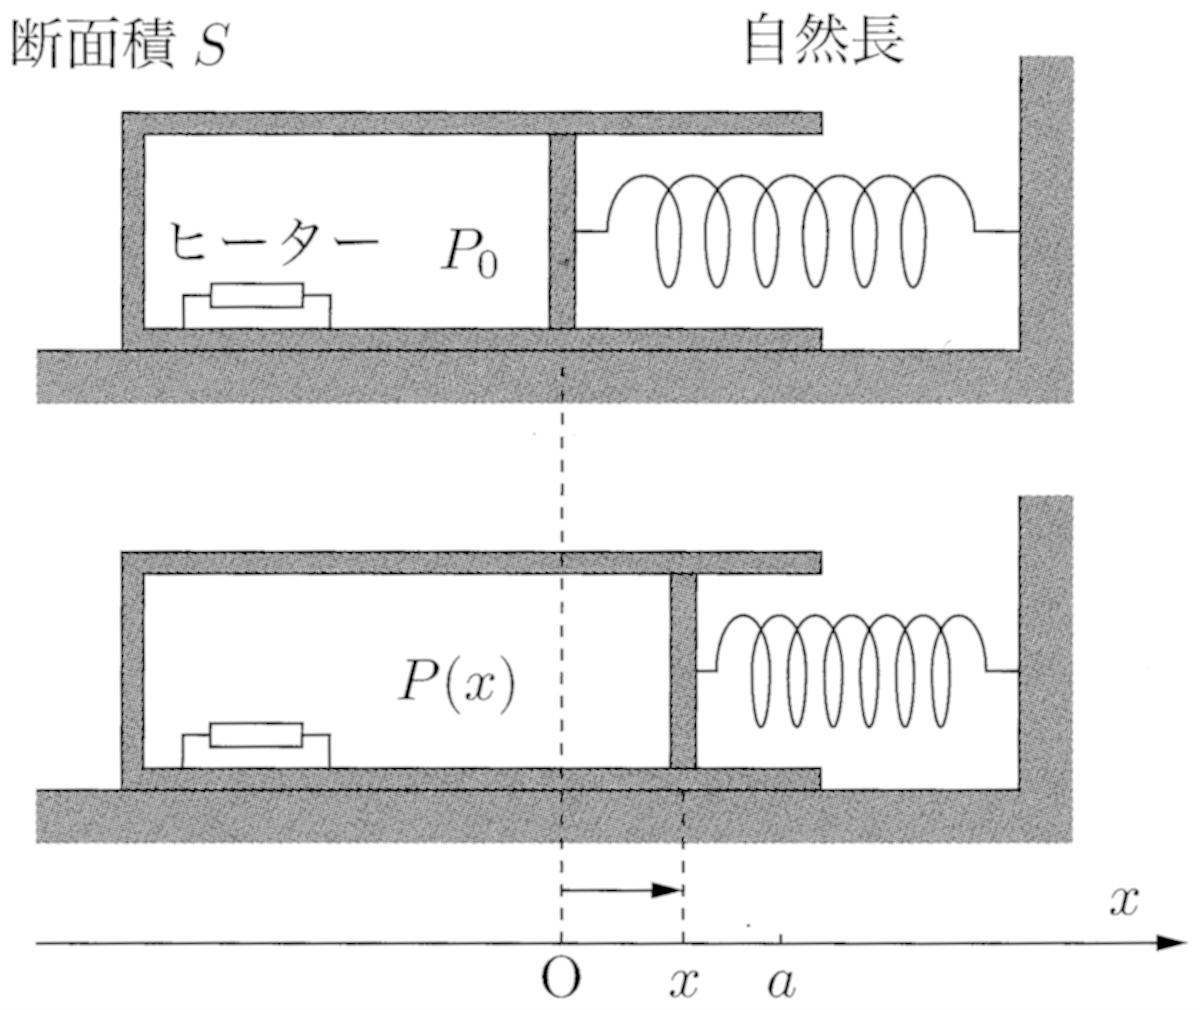
\includegraphics[keepaspectratio,width=68mm]{fig/ch16_ex8_cyl.png}
\end{zuright}
\begin{komon}
\ko{1} ピストンが位置$x\U{m}$にあるときの気体の圧力$P(x)\U{Pa}$を求めよ．
\ko{2} ピストンが$x\U{m}$から微小距離$dx\U{m}$だけ移動する間に気体が外界に対してする仕事$dw\U{J}$を求めよ．
\ko{3} この変化の$P$-$V$図を描け．ただし，$x=0\U{m}$のときの気体の体積を$V_0\U{m^3}$とする．
\ko{4} この状態変化で気体が外界に対してする全仕事$w\U{J}$を求めよ．
\end{komon}
\end{reidai}

\begin{sisinE}
ゆっくりと変化させているので，各瞬間でピストンに働く力はつり合っている．ピストンに働くのは，気体の圧力による力，大気圧による力，バネの弾性力の三つである．気体の圧力$P(x)$はこのつり合いの式から求まる．

体積と$x$は$V=V_0+Sx$，したがって$dV=S\,dx$で結ばれるので，$w=\displaystyle\int P\,dV$は$x$についての積分に書き換えて計算するとよい．
\end{sisinE}

\Key{ゆっくり変化させる $\Rightarrow$ ピストンはつり合いを保ちつつ変化する\quad $dw=P\,dV \rightarrow w=\displaystyle\int_{V_1}^{V_2}P\,dV$}

\begin{kaitou}
\begin{komon}
\ko{1} ピストンが位置$x$にあるとき，バネは自然長から$x$だけ縮んでおり，ピストンを左向きに$kx\U{N}$の力で押す．ピストンに働く力のつり合いより，
       \[P(x)S=P_0S+kx\]
       よって，
       \[P(x)=P_0+\frac{kx}{S}\U{Pa}\Ans\]
\ko{2} ピストンが$dx$だけ移動する間の気体の体積増加は$dV=S\,dx$であるから，
       \[dw=P(x)\,dV=\left(P_0+\frac{kx}{S}\right)S\,dx=(P_0S+kx)\,dx\U{J}\Ans\]
\ko{3} 気体の体積は$V=V_0+Sx$，すなわち$x=\dfrac{V-V_0}{S}$であるから，これを(1)に代入して
       \[P=P_0+\frac{k(V-V_0)}{S^2}\]
       となり，$P$は$V$の一次関数である．$x:0\rightarrow a$の変化であるから，体積は$V_0\rightarrow V_0+aS$，圧力は$P_0\rightarrow P_0+\dfrac{ka}{S}$と変化する．よって$P$-$V$図は次図．
       \begin{center}
       \ifbsAnaume
       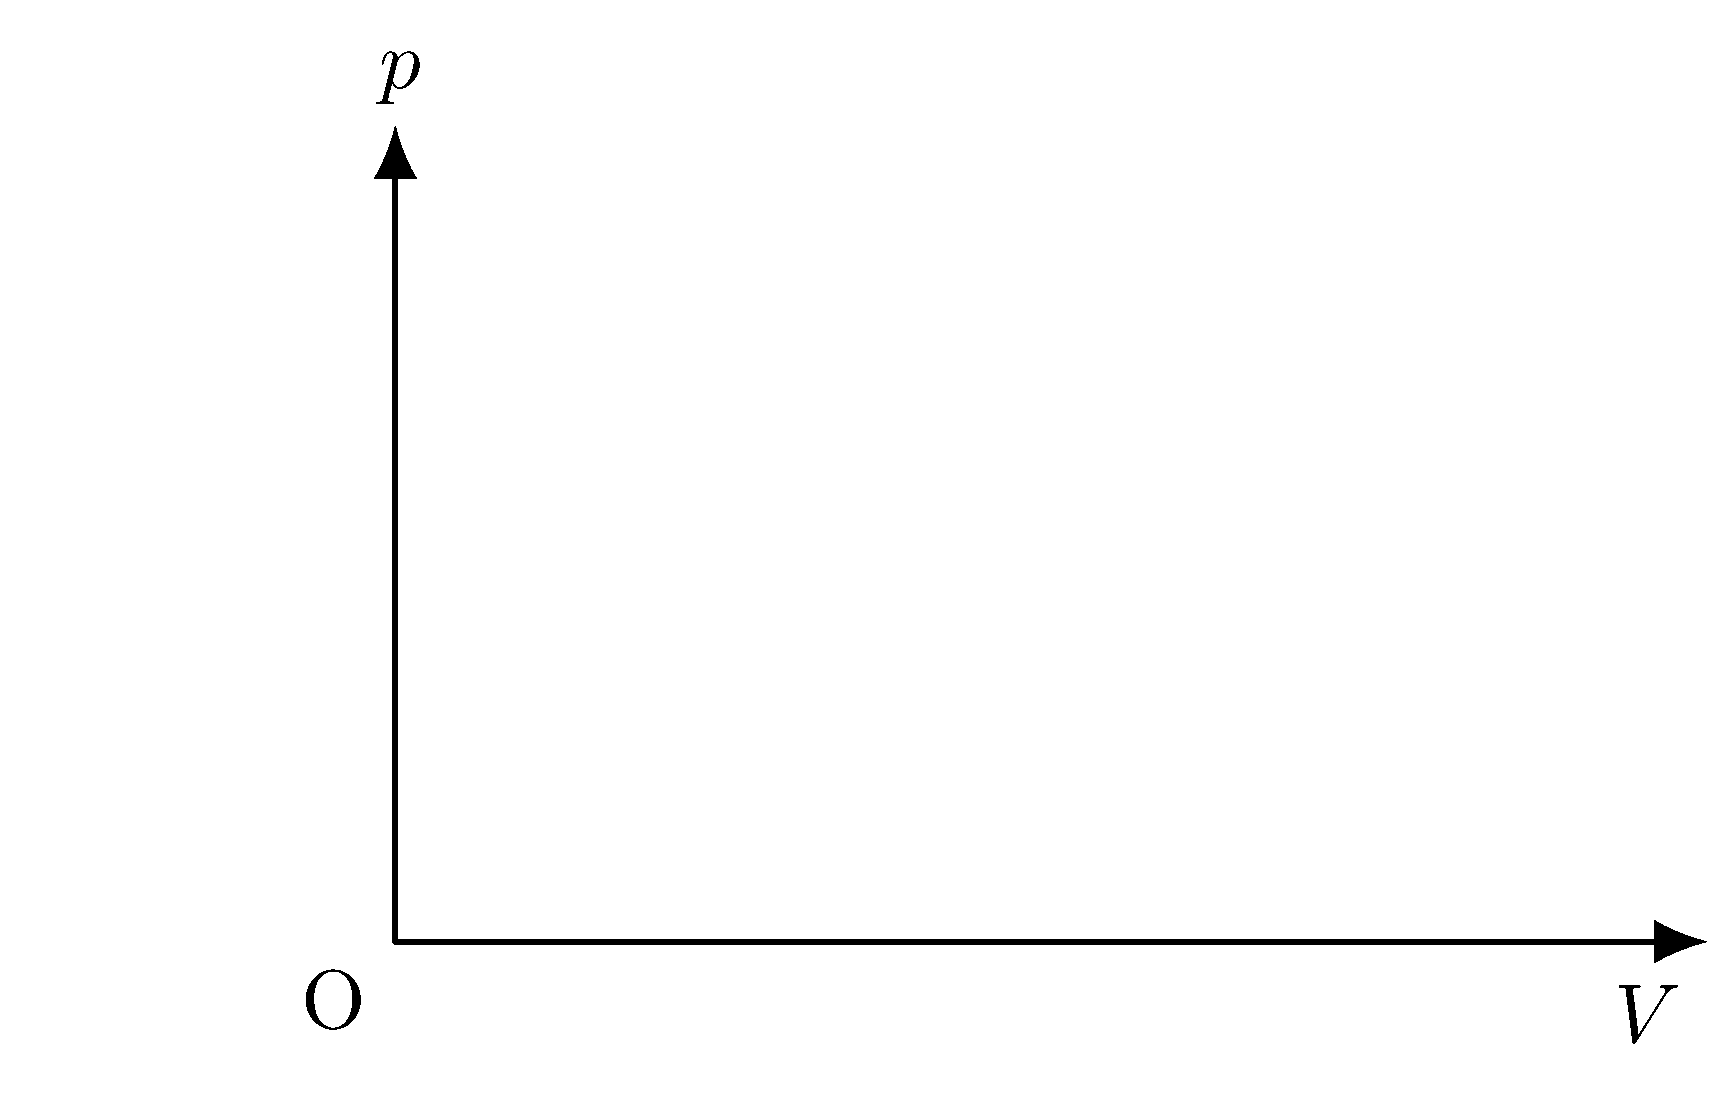
\includegraphics[keepaspectratio,width=72mm]{fig/ch16_ex8_pv_blank.png}
       \else
       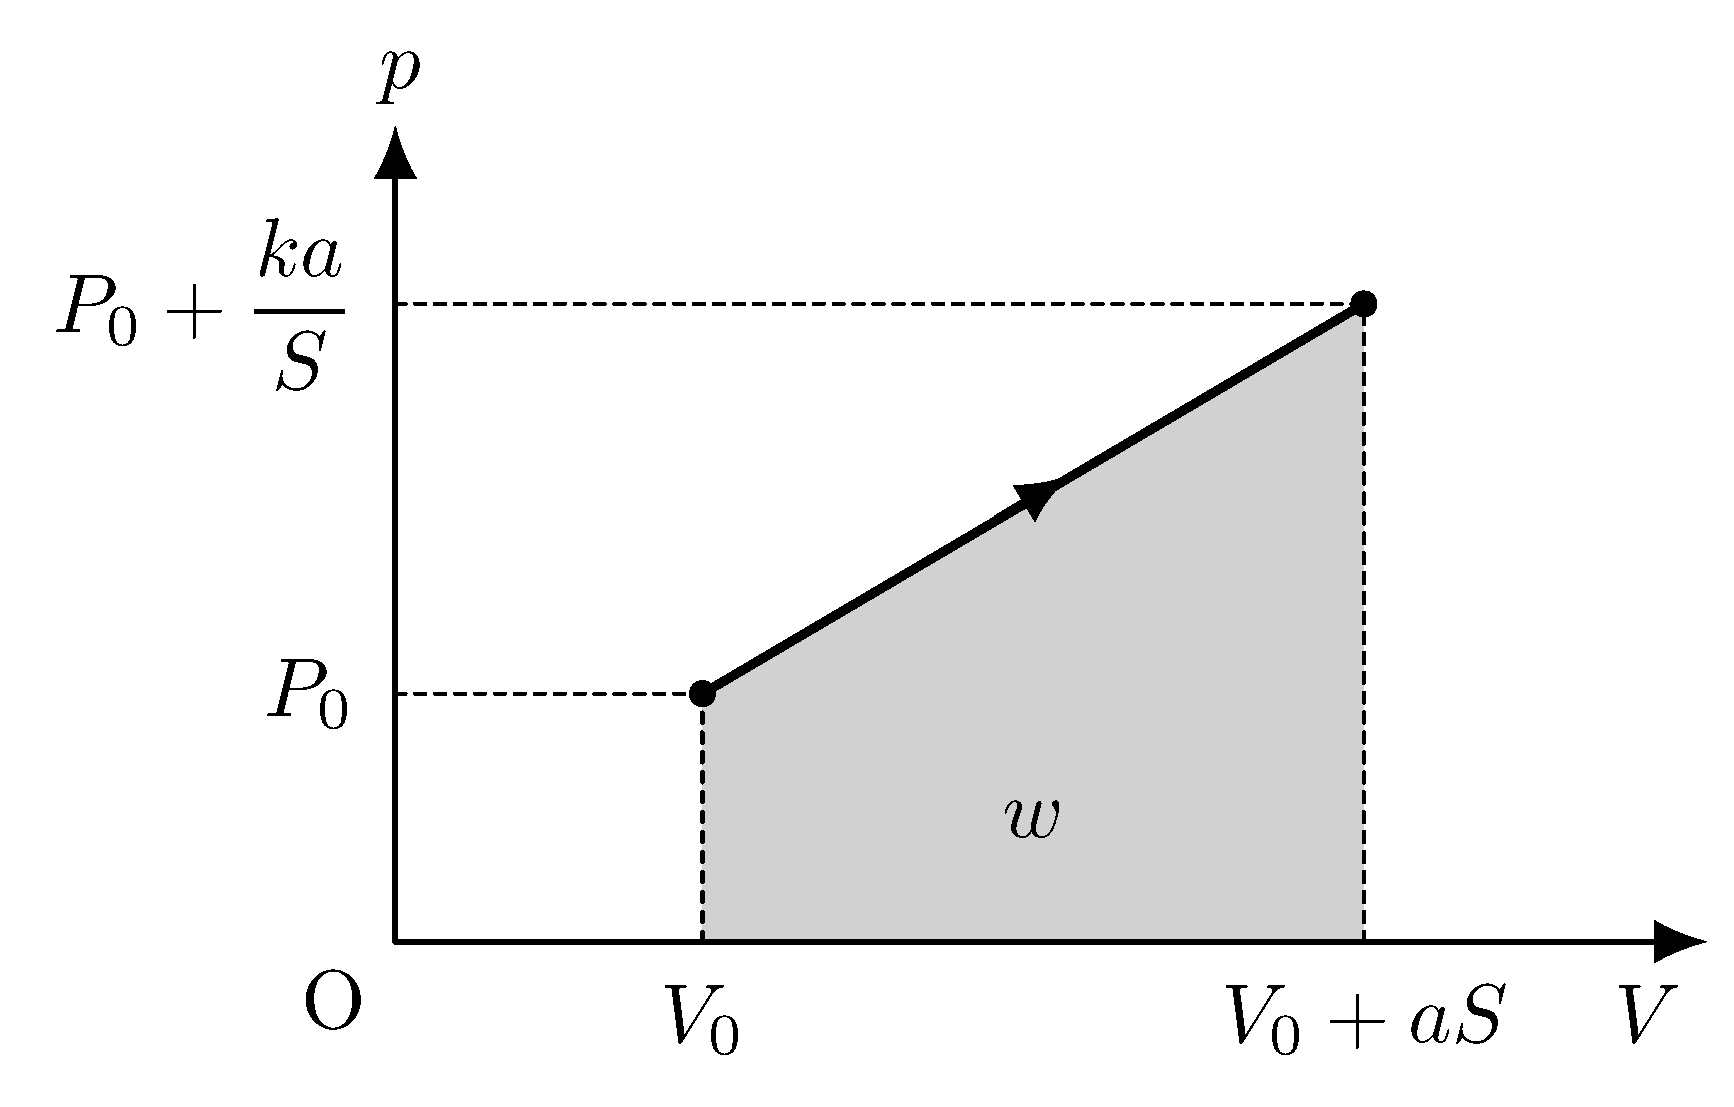
\includegraphics[keepaspectratio,width=72mm]{fig/ch16_ex8_pv.png}
       \fi
       \end{center}
       \hspace*{\fill}\Ans
\ko{4} (2)を$x:0\rightarrow a$の範囲で積分して，
       \Ana{w=\int_0^a(P_0S+kx)\,dx=P_0Sa+\frac{1}{2}ka^2\U{J}\Ans}
       \begin{chuu}
       (3)の$P$-$V$図は台形であるから，その面積として
       \[w=\frac{1}{2}\left\{P_0+\left(P_0+\frac{ka}{S}\right)\right\}\cdot aS=P_0Sa+\frac{1}{2}ka^2\U{J}\]
       と求めてもよい．積分と面積が同じものであることを確かめておくこと．
       \end{chuu}
\end{komon}
\end{kaitou}
\end{reidaiunit}
% 加筆（2026-09-21）：$P$-$V$図の面積として検算する注を足した．
%   23.1 で「積分＝面積」と述べた直後なので，ここで一度確かめさせたい．


\subsection{等温変化}

温度が一定に保たれる状態変化を{\gtfamily 等温変化}（定温変化）という．
気体を十分大きな一定温度の物体（熱浴）に接触させたままゆっくり変化させれば等温変化になる．

等温変化では温度が変化しないので内部エネルギーも変化せず，
\[\Delta U=nC_V\Delta T=0\]
である．
したがって熱力学第一法則$Q_{\mathrm{in}}=\Delta U+W_{\mathrm{out}}$より\,\AnaB{$Q_{\mathrm{in}}=W_{\mathrm{out}}$}\,，すなわち{\gtfamily 加えた熱はすべて気体が外界にする仕事になる}．

また，等温変化の途中では状態方程式より$P=\dfrac{nRT}{V}$であって圧力が体積とともに変化していくので，気体のする仕事は$W_{\mathrm{out}}=P\Delta V$とは書けない．
23.1の積分を実行すると，体積が$V_1\rightarrow V_2\U{m^3}$と変化する間に気体が外界にする仕事は，$nRT$が定数であることに注意して
\AnaBD{W_{\mathrm{out}}=\int_{V_1}^{V_2}\frac{nRT}{V}\,dV=nRT\Bigl[\log_e|V|\Bigr]_{V_1}^{V_2}=nRT\log_e\frac{V_2}{V_1}\U{J}}
となる．
$P$-$V$図では$PV=nRT=$（一定）の双曲線の一部となり，この曲線を\,\AnaB{等温曲線}\,と呼ぶ．

% 加筆（2026-09-21）：原本にはこのまとめ枠が無く，例題11・練習［25］［26］が毎回
%   同じ積分を最初から実行していた．結論を一度まとめておく．
\bsNeed{34mm}
\begin{matome}{等温変化}
 \hspace{3mm} $P$-$V$図は$PV=nRT=$（一定）の双曲線（{\gtfamily 等温曲線}）\\[1mm]
 \hspace{3mm} $\Delta U=0$\hspace{4mm} したがって\hspace{4mm} $Q_{\mathrm{in}}=W_{\mathrm{out}}$（加えた熱はすべて仕事になる）\\[1mm]
 \hspace{3mm} $W_{\mathrm{out}}=\displaystyle\int_{V_1}^{V_2}\frac{nRT}{V}\,dV=nRT\log_e\dfrac{V_2}{V_1}\U{J}$
\end{matome}

%%%%%%%%%%  例題11（23.2 の直後。原本の【例題11】）  %%%%%%%%%%%%%%%%%%%%
\bsNeed{96mm}
\begin{reidaiunit}
\begin{reidai}{等温変化}
\begin{zuright}{58mm}
\hspace{1zw}図のように一様な断面積を持つシリンダーに定積モル比熱が$C_V\U{J/mol\cdot K}$の理想気体を$n\U{mol}$封入した．ピストンは軽くて自由に動くことができ，棒が取り付けてある．最初，この気体の温度は$T_0\U{K}$，体積は$V_0\U{m^3}$であった．
\par
\hspace{1zw}シリンダー内にはヒーターが取り付けてあり，気体に対して熱を与えることができる．シリンダーおよびピストンは断熱材で出来ており，ヒーターによって与えた熱が大気に逃げることはないものとする．気体定数を$R\U{J/mol\cdot K}$として以下の問に答えよ．
\zusep
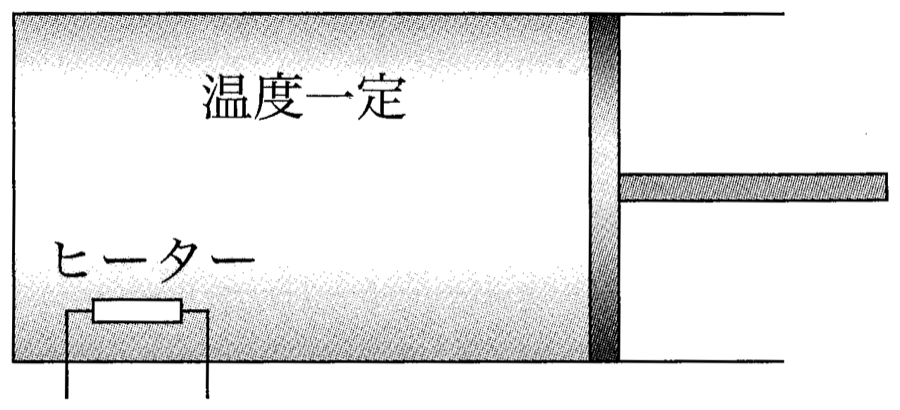
\includegraphics[keepaspectratio,width=58mm]{fig/ch17_ex11_cyl.png}
\end{zuright}
\begin{komon}
\ko{1} 始めの状態における気体の圧力$P_0\U{Pa}$を求めよ．
\end{komon}
\hspace{1zw}ここで，気体が温度$T_0\U{K}$を保つようにピストンを操作しながら気体に熱をゆっくりと与え，体積を$V_1\U{m^3}$となるまで膨張させた．
\begin{komon}
\ko{2} 終状態における気体の圧力$P_1\U{Pa}$を求めよ．
\ko{3} 気体の体積が$V\U{m^3}$（$V_0<V<V_1$）のときの気体の圧力$P(V)\U{Pa}$を求めよ．
\ko{4} この状態変化を$P$-$V$図で表せ．
\ko{5} この変化において気体が外界に対してした仕事$w\U{J}$を求めよ．ただし，$\displaystyle\int\frac{1}{x}dx=\log_e|x|+C$（$C$は積分定数）である．
\ko{6} この変化における気体の内部エネルギーの増加量$\Delta U\U{J}$を求めよ．
\ko{7} ヒーターによって加えた熱量$Q\U{J}$を求めよ．
\end{komon}
\end{reidai}

\begin{sisinE}
温度が一定に保たれる状態変化を{\gtfamily 等温変化}という．等温変化では内部エネルギーが変化しないので，加えた熱はすべて気体が外界にする仕事になる．

(5) この状態変化では圧力$P$は一定ではないから，$w=P\Delta V$とは書けないことに注意せよ．体積が$V\U{m^3}$のときの圧力$P(V)$を求め，それを積分する．
\end{sisinE}

\Key{状態方程式 $PV=nRT$\quad 内部エネルギー変化 $\Delta U=nC_V\Delta T$\quad 気体のする仕事 $w=\displaystyle\int_{V_1}^{V_2}P\,dV$\quad 熱力学第一法則 $Q=\Delta U+w$}

\begin{kaitou}
\begin{komon}
\ko{1} 始めの状態の状態方程式$P_0V_0=nRT_0$より，
       \[P_0=\frac{nRT_0}{V_0}\U{Pa}\Ans\]
\ko{2} 終状態でも温度は$T_0$のままであるから，状態方程式$P_1V_1=nRT_0$より，
       \[P_1=\frac{nRT_0}{V_1}\U{Pa}\Ans\]
\ko{3} 体積が$V$のときも温度は$T_0$であるから，状態方程式$P(V)\cdot V=nRT_0$より，
       \[P(V)=\frac{nRT_0}{V}\U{Pa}\Ans\]
\ko{4} (3)より$P$-$V$図は$PV=nRT_0$（一定）の双曲線の一部で，次図の通り．
       \begin{center}
       \ifbsAnaume
       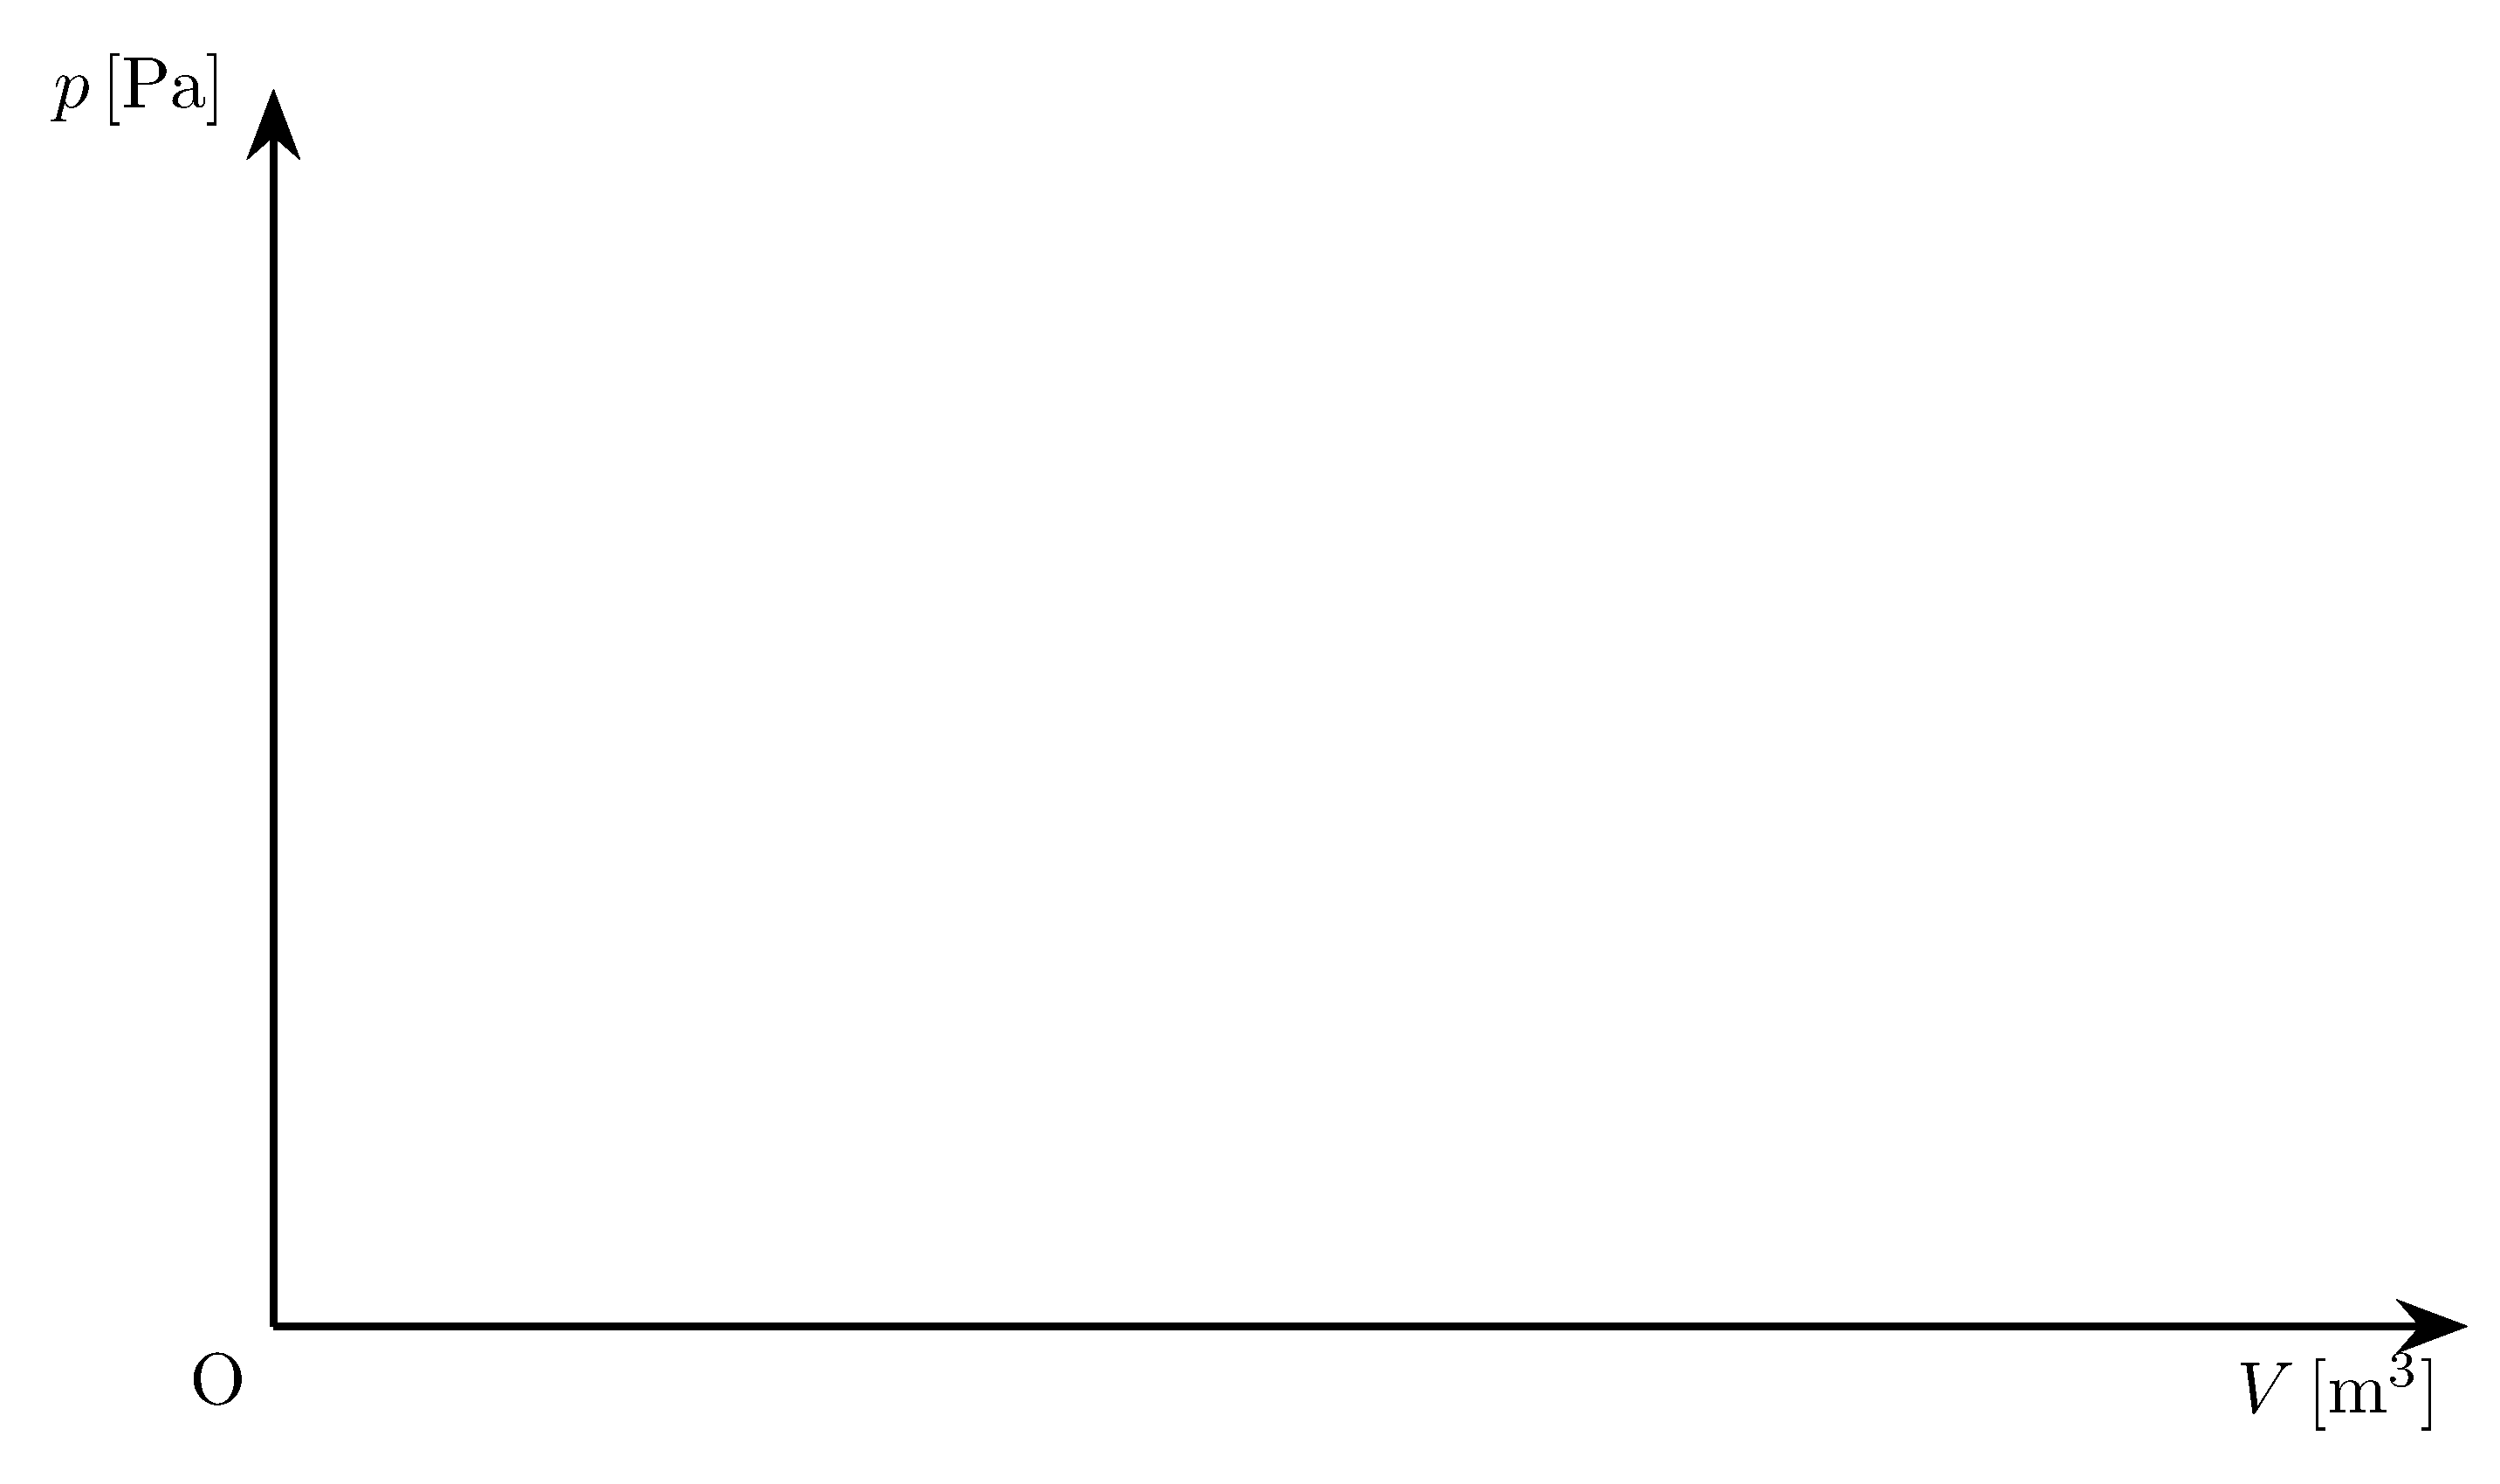
\includegraphics[keepaspectratio,width=96mm]{fig/ch17_ex11_pv_blank.png}
       \else
       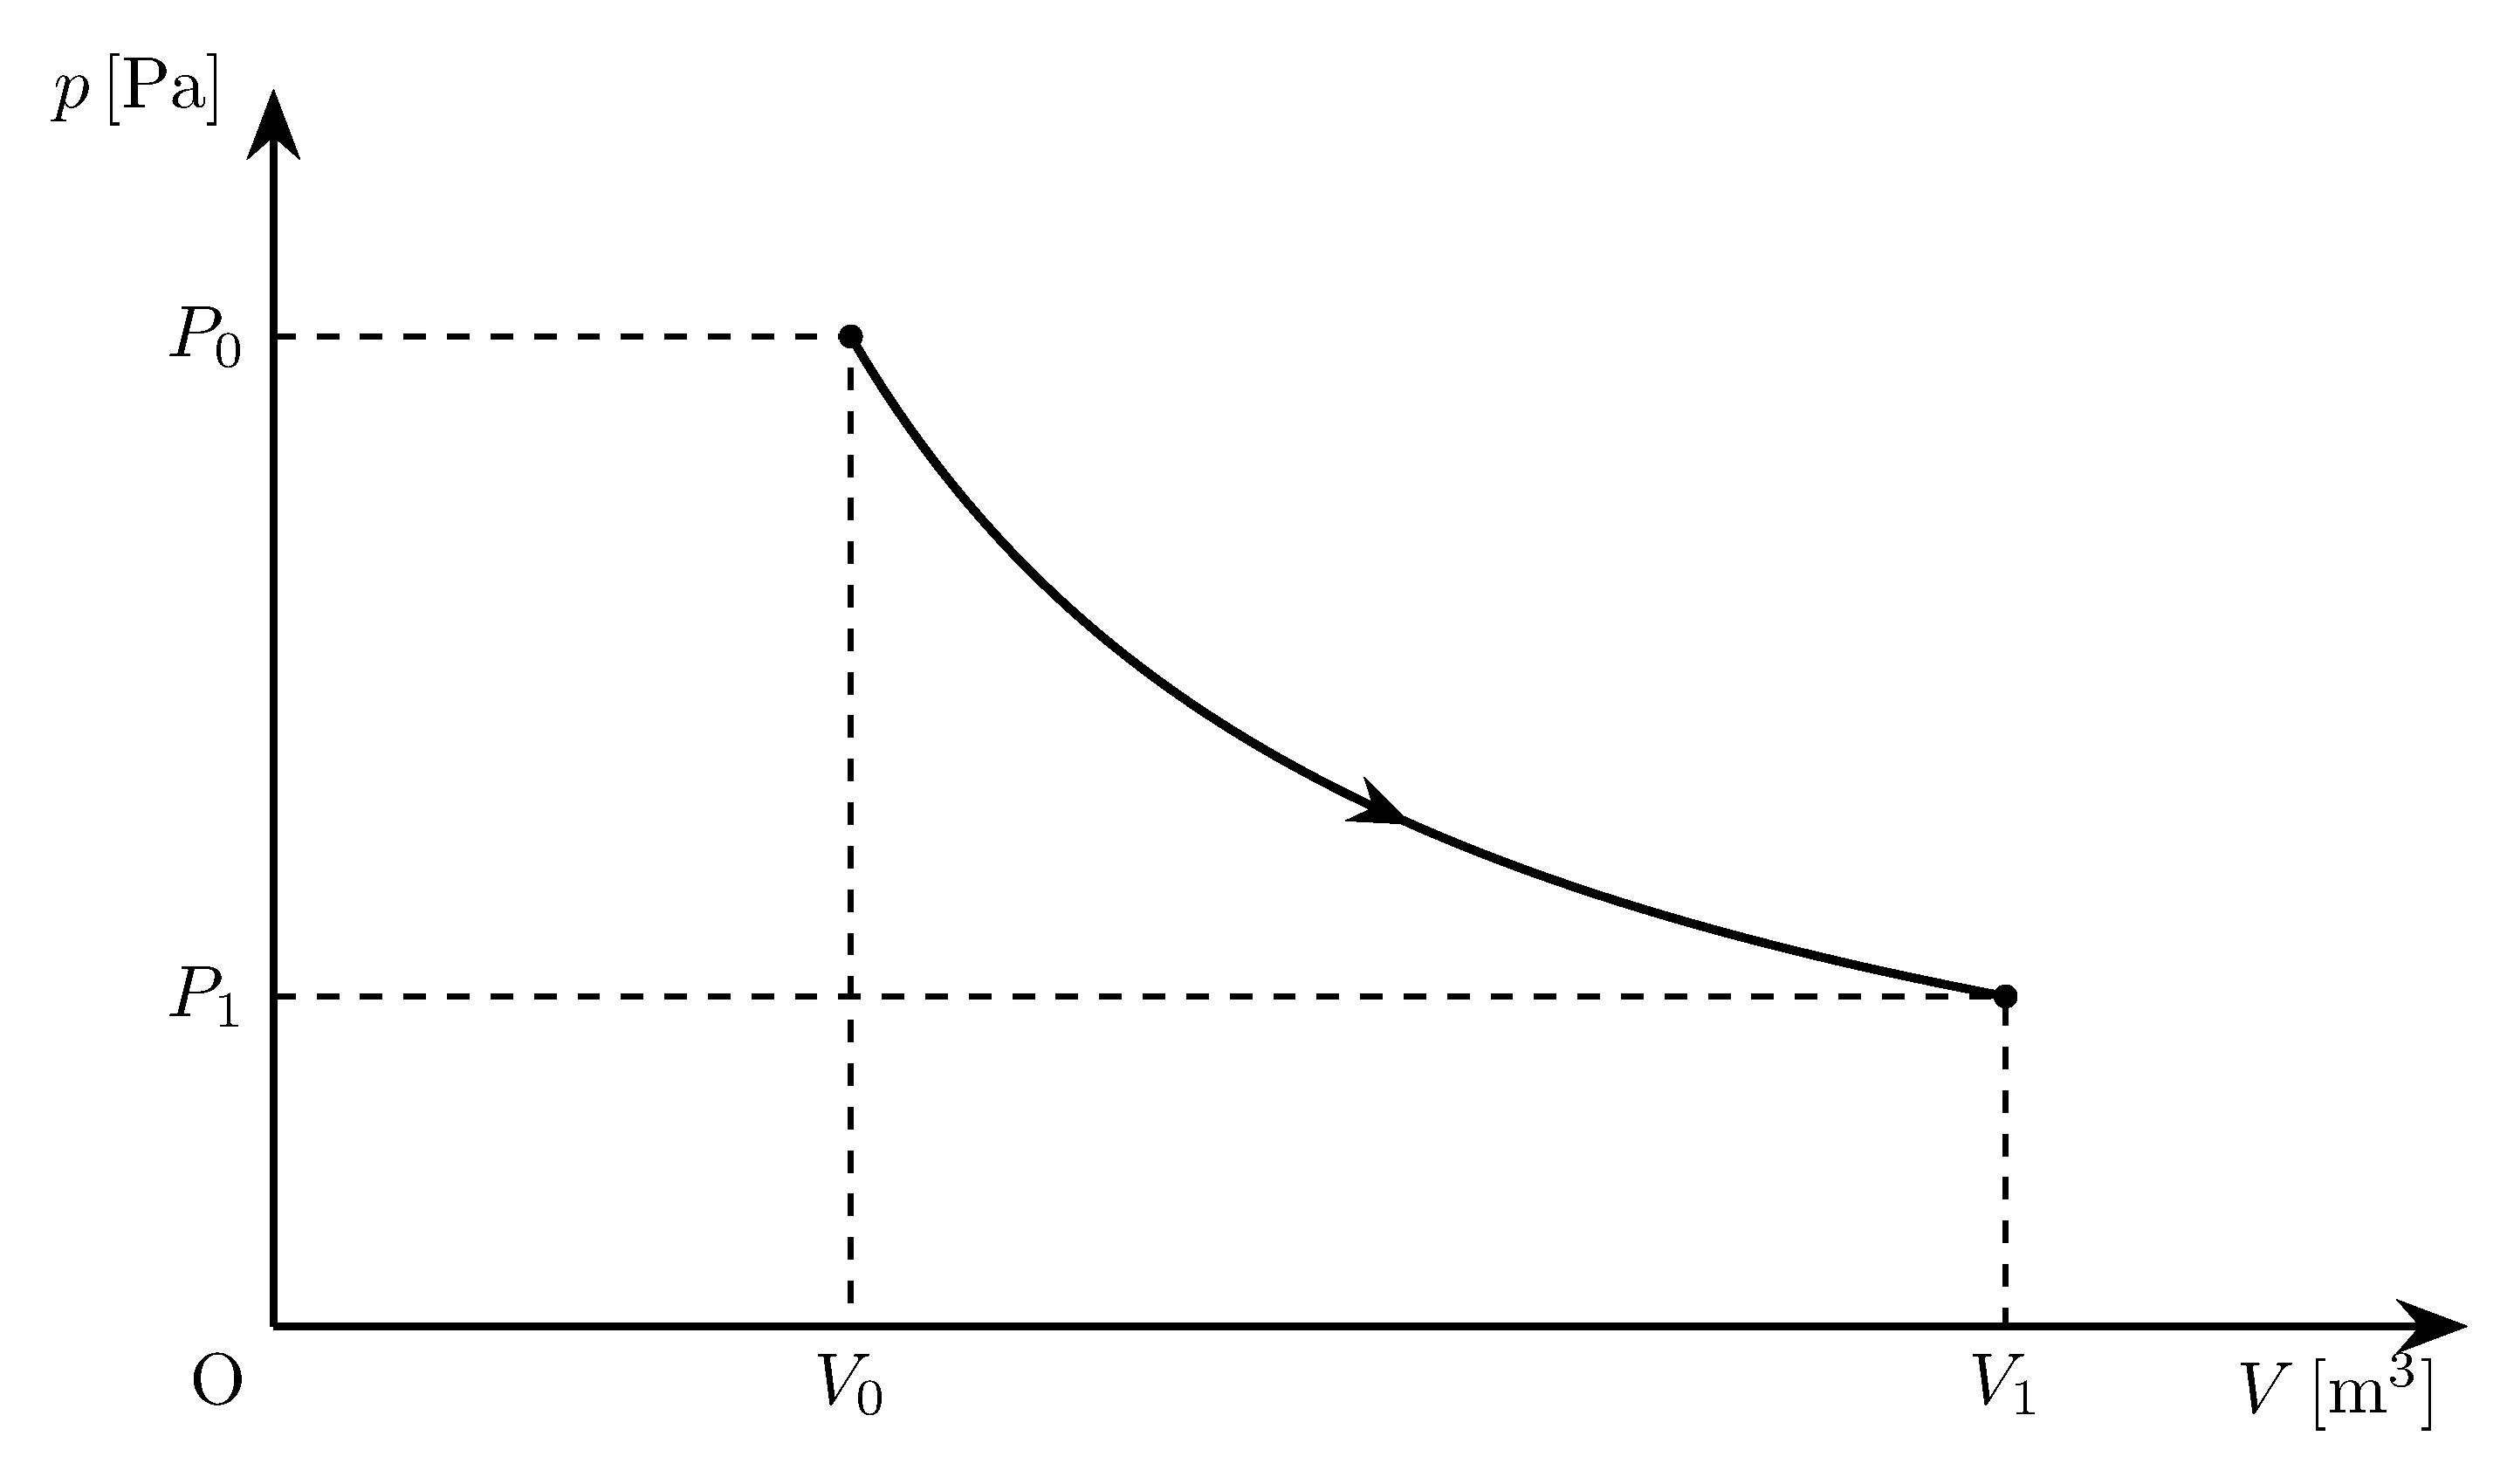
\includegraphics[keepaspectratio,width=96mm]{fig/ch17_ex11_pv.png}
       \fi
       \end{center}
       \hspace*{\fill}\Ans
\ko{5} $nRT_0$は定数であることに注意して，
       \[w=\int_{V_0}^{V_1}P(V)dV=nRT_0\int_{V_0}^{V_1}\frac{1}{V}dV
             =nRT_0\log_e\frac{V_1}{V_0}\U{J}\Ans\]
\ko{6} 温度が$T_0$のまま変化しないので$\Delta T=0$であり，
       \[\Delta U=nC_V\Delta T=0\U{J}\Ans\]
\ko{7} 熱力学第一法則$Q=\Delta U+w$より，
       \Ana{Q=nRT_0\log_e\frac{V_1}{V_0}\U{J}\Ans}
       すなわち，加えた熱はすべて気体が外界にした仕事になっている．
\end{komon}
\end{kaitou}
\end{reidaiunit}


\subsection{断熱変化}

外部との熱の出入りを遮断して気体を状態変化させることを{\gtfamily 断熱変化}という．
断熱材で囲んでしまうか，熱のやりとりが間に合わないほど速く変化させれば断熱変化になる．

% 加筆（2026-09-21 レビュー）：「断熱変化では温度が下がる」と「断熱自由膨張では温度が変わらない」
%   が数ページ後にぶつかるので，はじめに $Q_{in}=0$ の中を2つに分けておく．
断熱変化とは$Q_{\mathrm{in}}=0$の変化のことであるが，その中身は次の2つに分かれる．
\begin{quote}
\noindent\MARU{1}\ ピストンをゆっくり動かす{\gtfamily 準静的な断熱膨張・圧縮}（本節）\\
\MARU{2}\ 真空へ噴き出す{\gtfamily 断熱自由膨張}（23.4）
\end{quote}
\noindent 同じ「断熱」でも結論はまるで違う（\MARU{1}では温度が変わり，\MARU{2}では変わらない）ので，はじめに区別しておく．
本節で扱うのは\MARU{1}であり，あとで述べるポアソンの式が使えるのも\MARU{1}だけである．

% 加筆（2026-09-21）：原本は「断熱変化では圧力，体積，温度の全てが変化する」の一文だけで，
%   W_out=-ΔU は練習［27］の指針で初めて出てくる．ここに上げた．
断熱変化では$Q_{\mathrm{in}}=0$であるから，熱力学第一法則は
\AnaBD{0=\Delta U+W_{\mathrm{out}}\hspace{5mm}\Longleftrightarrow\hspace{5mm} W_{\mathrm{out}}=-\Delta U=-nC_V\Delta T}
となる．
{\gtfamily 断熱変化に限り，仕事$W_{\mathrm{out}}$を積分せずに内部エネルギーの変化だけから求められる}のがポイントである．
またこの式は，{\gtfamily 断熱膨張（$W_{\mathrm{out}}>0$）では必ず温度が下がり，断熱圧縮（$W_{\mathrm{out}}<0$）では必ず温度が上がる}ことを意味している．
なお{\gtfamily 準静的な}断熱膨張・圧縮では圧力・体積・温度のいずれも変化することに注意せよ．

これは分子の運動から見ても納得できる．
第22回の練習［21］では，近づいてくるピストンに分子が弾性衝突するとはね返る速さが大きくなり，断熱圧縮で温度が上がることを見た．
膨張のときはその逆で，遠ざかるピストンに衝突した分子は速さを失う（＝気体が外界に仕事をする）ので，温度が下がるのである．

%%%%%%%%%%  例題12（23.3 の前半。原本の【例題12】）  %%%%%%%%%%%%%%%%%%%%
\bsNeed{64mm}
\begin{reidaiunit}
\begin{reidai}{断熱変化}
\hspace{1zw}始状態において圧力$P_0\U{Pa}$，体積$V_0\U{m^3}$の理想気体を，外部との熱のやり取りを断ったまま体積が$V_1\U{m^3}$（ただし$V_1>V_0$）になるまで変化させる．終状態における気体の圧力を$P_1\U{Pa}$，気体定数を$R\U{J/mol\cdot K}$，気体の定積モル比熱を$C_V\U{J/mol\cdot K}$として以下の問に答えよ．
\begin{komon}
\ko{1} 内部エネルギー変化$\Delta U\U{J}$，気体が外にした仕事$w\U{J}$，吸熱量$Q\U{J}$を求めよ．
\ko{2} 膨張過程なので$w>0$である事を利用して，この変化によって気体の温度は増加するか，減少するか，答えよ．
\end{komon}
\end{reidai}

\begin{sisinE}
熱の出入りを断った状態変化なので$Q=0$である．与えられているのは$P$と$V$だけで温度が与えられていないが，状態方程式$PV=nRT$を使えば$nRT$を$PV$に置き換えられるので，$\Delta U=nC_V\Delta T$は$P$, $V$だけで表せる．
\end{sisinE}

\begin{kaitou}
\begin{komon}
\ko{1} 断熱変化であるから，
       \[Q=0\U{J}\Ans\]
       気体のモル数を$n\U{mol}$，始状態・終状態の温度を$T_0\U{K}$, $T_1\U{K}$とすると，状態方程式より$P_0V_0=nRT_0$, $P_1V_1=nRT_1$であるから，
       \[\Delta U=nC_V(T_1-T_0)=\frac{C_V}{R}(P_1V_1-P_0V_0)\U{J}\Ans\]
       熱力学第一法則$Q=\Delta U+w$に$Q=0$を代入して，
       \[w=-\Delta U=\frac{C_V}{R}(P_0V_0-P_1V_1)\U{J}\Ans\]
\ko{2} (1)より$\Delta U=-w$であり，$w>0$であるから$\Delta U<0$である．$\Delta U=nC_V\Delta T$で$nC_V>0$であるから$\Delta T<0$，すなわち気体の温度は\AnaU{\gtfamily 減少する}．\hspace*{\fill}\Ans
\end{komon}
\end{kaitou}
\end{reidaiunit}

準静的な断熱変化では圧力，体積，温度の全てが変化するが，終状態は1通りしか取れないため，例題12の終状態の圧力$P_1\U{Pa}$は与えられた文字を用いて表すことが出来るはずである．
この値を求めるためには以下に示す{\gtfamily ポアソンの法則}を利用する．

\bsNeed{40mm}
\begin{matome}{ポアソンの法則}
 \hspace{3mm} 準静的な断熱変化の間は，比熱比$\gamma=\dfrac{C_P}{C_V}\ (>1)$を用いて
\AnaBD{PV^\gamma=（一定）\hspace{8mm} TV^{\gamma-1}=（一定）}
 が成立する．\\[0.5mm]
 \hspace{3mm} マイヤーの関係式$C_P=C_V+R$より，$\gamma=1+\dfrac{R}{C_V}$，すなわち$\gamma-1=$\,\AnaB{$\dfrac{R}{C_V}$}\,である．
\end{matome}
% 加筆（2026-09-21）：γ−1=R/C_V を枠に入れた．例題13(5)・練習［27］(2) の両方が
%   これを毎回導き直していたが，ポアソンの式とセットで覚えるべきもの．

この法則を微小変化に注目して導出してみよう．

\begin{zuright}{56mm}
\hspace{1zw}体積$V\U{m^3}$のときの圧力を$P\U{Pa}$として，微小体積$\Delta V\U{m^3}$分の気体を断熱膨張させると，この間に気体が外にした微小仕事は
\[\Delta W=P\Delta V\]
となる．
この変化の前後で圧力が$\Delta P\U{Pa}$，温度が$\Delta T\U{K}$だけ変化したとすると，断熱変化なので熱力学第一法則より
\zusep

\includegraphics[keepaspectratio,width=56mm]{text_p79_fig1.png}
\end{zuright}

\[0=nC_V\Delta T+\Delta W \hspace{5mm} \Leftrightarrow \hspace{5mm} nC_V\Delta T=-P\Delta V\]

ここで，断熱膨張前後の状態方程式より
\[PV=nRT\]
\[(P+\Delta P)(V+\Delta V)=nR(T+\Delta T)\]

第2式において二次の微小量$\Delta P\Delta V$を無視して第1式を利用すれば
\[PV+P\Delta V +\Delta P\cdot V=nRT+nR\Delta T\]
\[\Leftrightarrow \hspace{3mm} P\Delta V +\Delta P\cdot V=nR\Delta T\]
熱力学第一法則の式に代入して
\[\dfrac{C_V}{R}(P\Delta V+\Delta P\cdot V)=-P\Delta V \hspace{5mm} \Leftrightarrow \hspace{5mm} \dfrac{C_V+R}{C_V}\cdot\dfrac{\Delta V}{V}=-\dfrac{\Delta P}{P}\]

マイヤーの関係式より$C_P=C_V+R$なので，$\dfrac{C_V+R}{C_V}=\gamma$と置き換えられる．
これを両辺積分すると，積分定数を$D$として
\[\gamma \log_e V=-\log_e P+D \hspace{5mm} \Leftrightarrow \hspace{5mm} \log_e PV^\gamma =D \hspace{5mm} \Leftrightarrow \hspace{5mm} PV^\gamma =e^D\]

$e^D$は定数なので，$PV^\gamma =（一定）$が成立する．

また，$PV^\gamma =（一定）$と状態方程式$PV=nRT$を合わせて
\[\dfrac{nRT}{V}V^\gamma =（一定）\hspace{5mm} \Leftrightarrow \hspace{5mm} TV^{\gamma -1}=（一定）\]
も示すことができる．

\begin{zuright}{56mm}
\hspace{1zw}等温変化では状態方程式より$PV=（一定）$が成立するのに対し，断熱変化では$PV^\gamma=（一定）$で$\gamma>1$であるから，同じ点を通る2本の曲線を比べると\,\AnaB{断熱曲線}\,の方が等温曲線より傾きが急になる．
膨張させたとき，等温曲線では温度が保たれるのに対し，断熱曲線では温度も下がるぶんだけ圧力が余計に下がるからである．
\zusep

\includegraphics[keepaspectratio,width=56mm]{text_p80_fig1.png}
\end{zuright}
% 加筆（2026-09-21）：原本は「傾きが大きい曲線となることがわかる」と結果だけだった．
%   理由（膨張で温度も下がるぶん圧力が余計に下がる）を1文足した．

%%%%%%%%%%  例題13（23.3 の後半。原本の【例題13】）  %%%%%%%%%%%%%%%%%%%%
\bsNeed{88mm}
\begin{reidaiunit}
\begin{reidai}{ポアソンの式の利用}
\begin{zuright}{50mm}
\hspace{1zw}図のように一様な断面積を持つシリンダーに定積モル比熱が$C_V\U{J/mol\cdot K}$の理想気体を$n\U{mol}$封入した．ピストンは軽くて自由に動くことができ，外気圧とシリンダー内の気体の圧力とが常につり合いを保つ．シリンダーおよびピストンは断熱材で出来ており，外界との熱のやり取りはない．最初，この気体の温度は$T_0\U{K}$，体積は$V_0\U{m^3}$であり，ピストンは静止していた．
\zusep
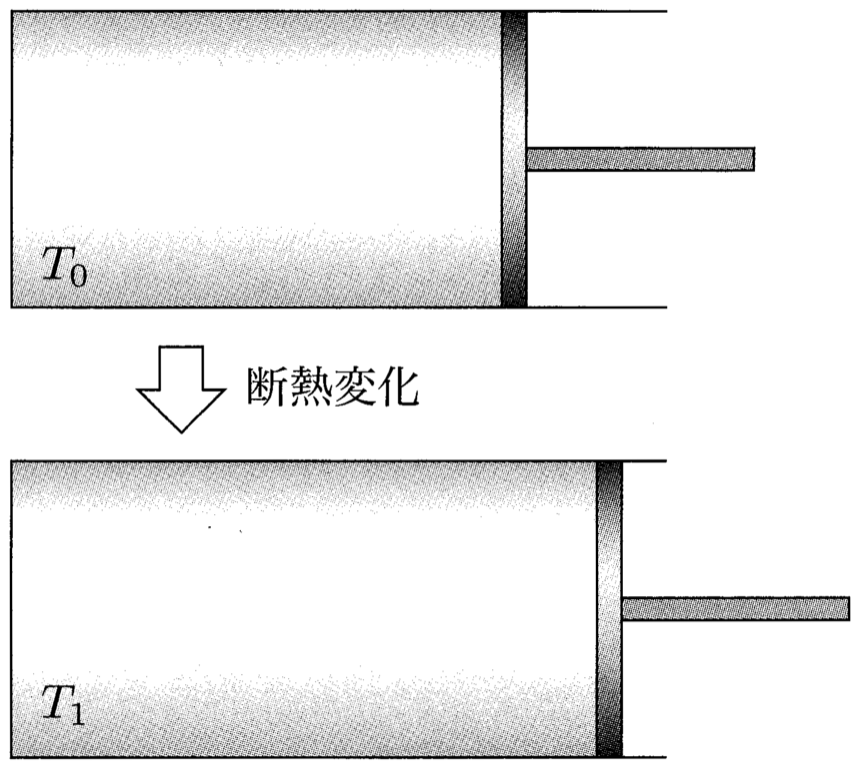
\includegraphics[keepaspectratio,width=50mm]{fig/ch17_ex13_cyl.png}
\end{zuright}
\hspace{1zw}この状態から外気圧をゆっくりと変化させ，気体の温度が$T_1\U{K}$($<T_0$)となるまで変化させた．理想気体が断熱変化するときは比熱比を$\gamma$として，ポアソンの式$PV^\gamma=（一定）$が成立することを用いてよい．気体定数を$R\U{J/mol\cdot K}$として以下の問に答えよ．
\begin{komon}
\ko{1} この状態変化を$P$-$V$図で表せ．ただし，終状態の体積を$V_1\U{m^3}$として図示せよ．
\ko{2} この気体が始状態から定温条件で体積$V_1\U{m^3}$となるまで変化した場合，気体はどのような曲線上を動くか．(1)の$P$-$V$図に点線で記入せよ．
\ko{3} この気体の内部エネルギー変化$\Delta U\U{J}$を求めよ．
\ko{4} この気体が外界にした仕事$w\U{J}$を求めよ．
\ko{5} 終状態における気体の体積$V_1\U{m^3}$を求めよ．
\end{komon}
\end{reidai}

\begin{sisinE}
温度が下がる断熱変化であるから，気体は外界に仕事をして膨張する（$V_1>V_0$）．$P$-$V$図では断熱曲線は等温曲線より急な右下がりの曲線になるので，同じ体積$V_1$まで変化させたとき断熱変化の方が圧力は低い．

断熱変化では$Q=0$なので，仕事$w$は積分せずとも熱力学第一法則$Q=\Delta U+w$から求まる．体積を問われている(5)では，$P$と$V$を結ぶ$PV^\gamma=（一定）$ではなく$T$と$V$を結ぶ$TV^{\gamma-1}=（一定）$を使う．
\end{sisinE}

\Key{断熱変化中は比熱比$\gamma=\dfrac{C_P}{C_V}$を用いて $PV^\gamma=（一定）$, $TV^{\gamma-1}=（一定）$ が成立する}

\begin{kaitou}
\begin{komon}
\item[{\makebox[1.9zw][r]{(1)(2)}}] 断熱変化（実線）は$PV^\gamma=（一定）$，等温変化（点線）は$PV=（一定）$の曲線である．$\gamma>1$であるから断熱曲線の方が急になり，次図の通り．
       \begin{center}
       \ifbsAnaume
       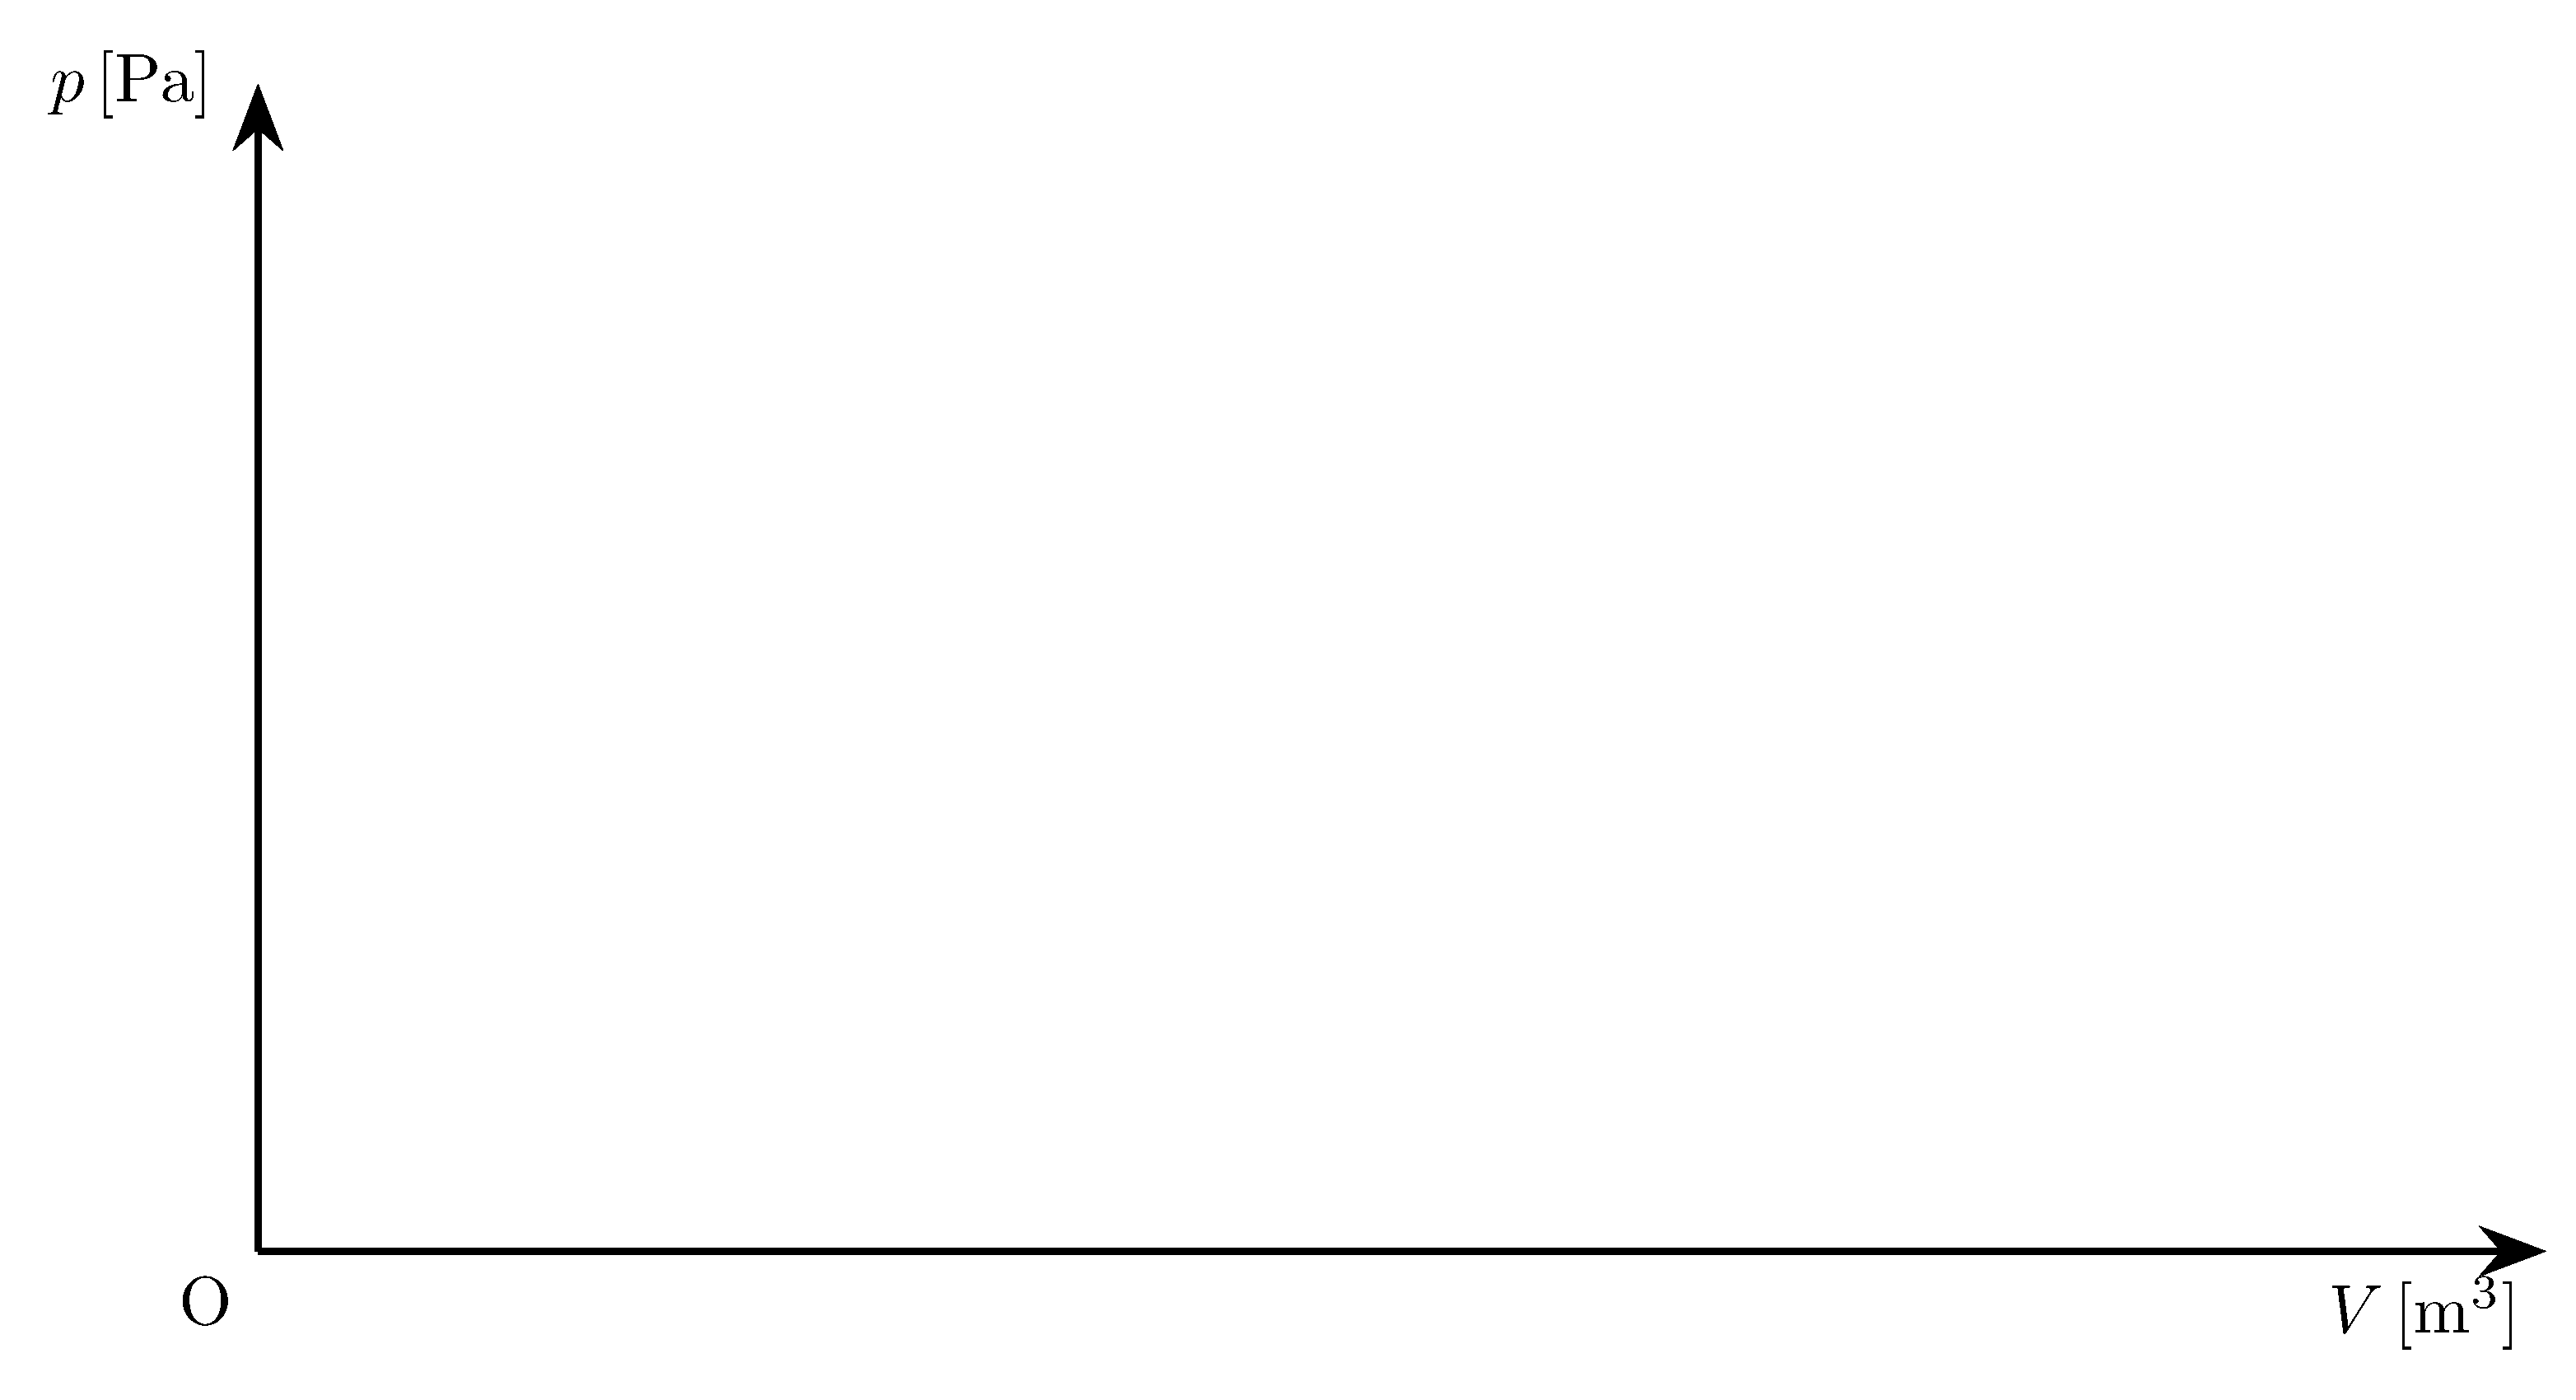
\includegraphics[keepaspectratio,width=106mm]{fig/ch17_ex13_pv_blank.png}
       \else
       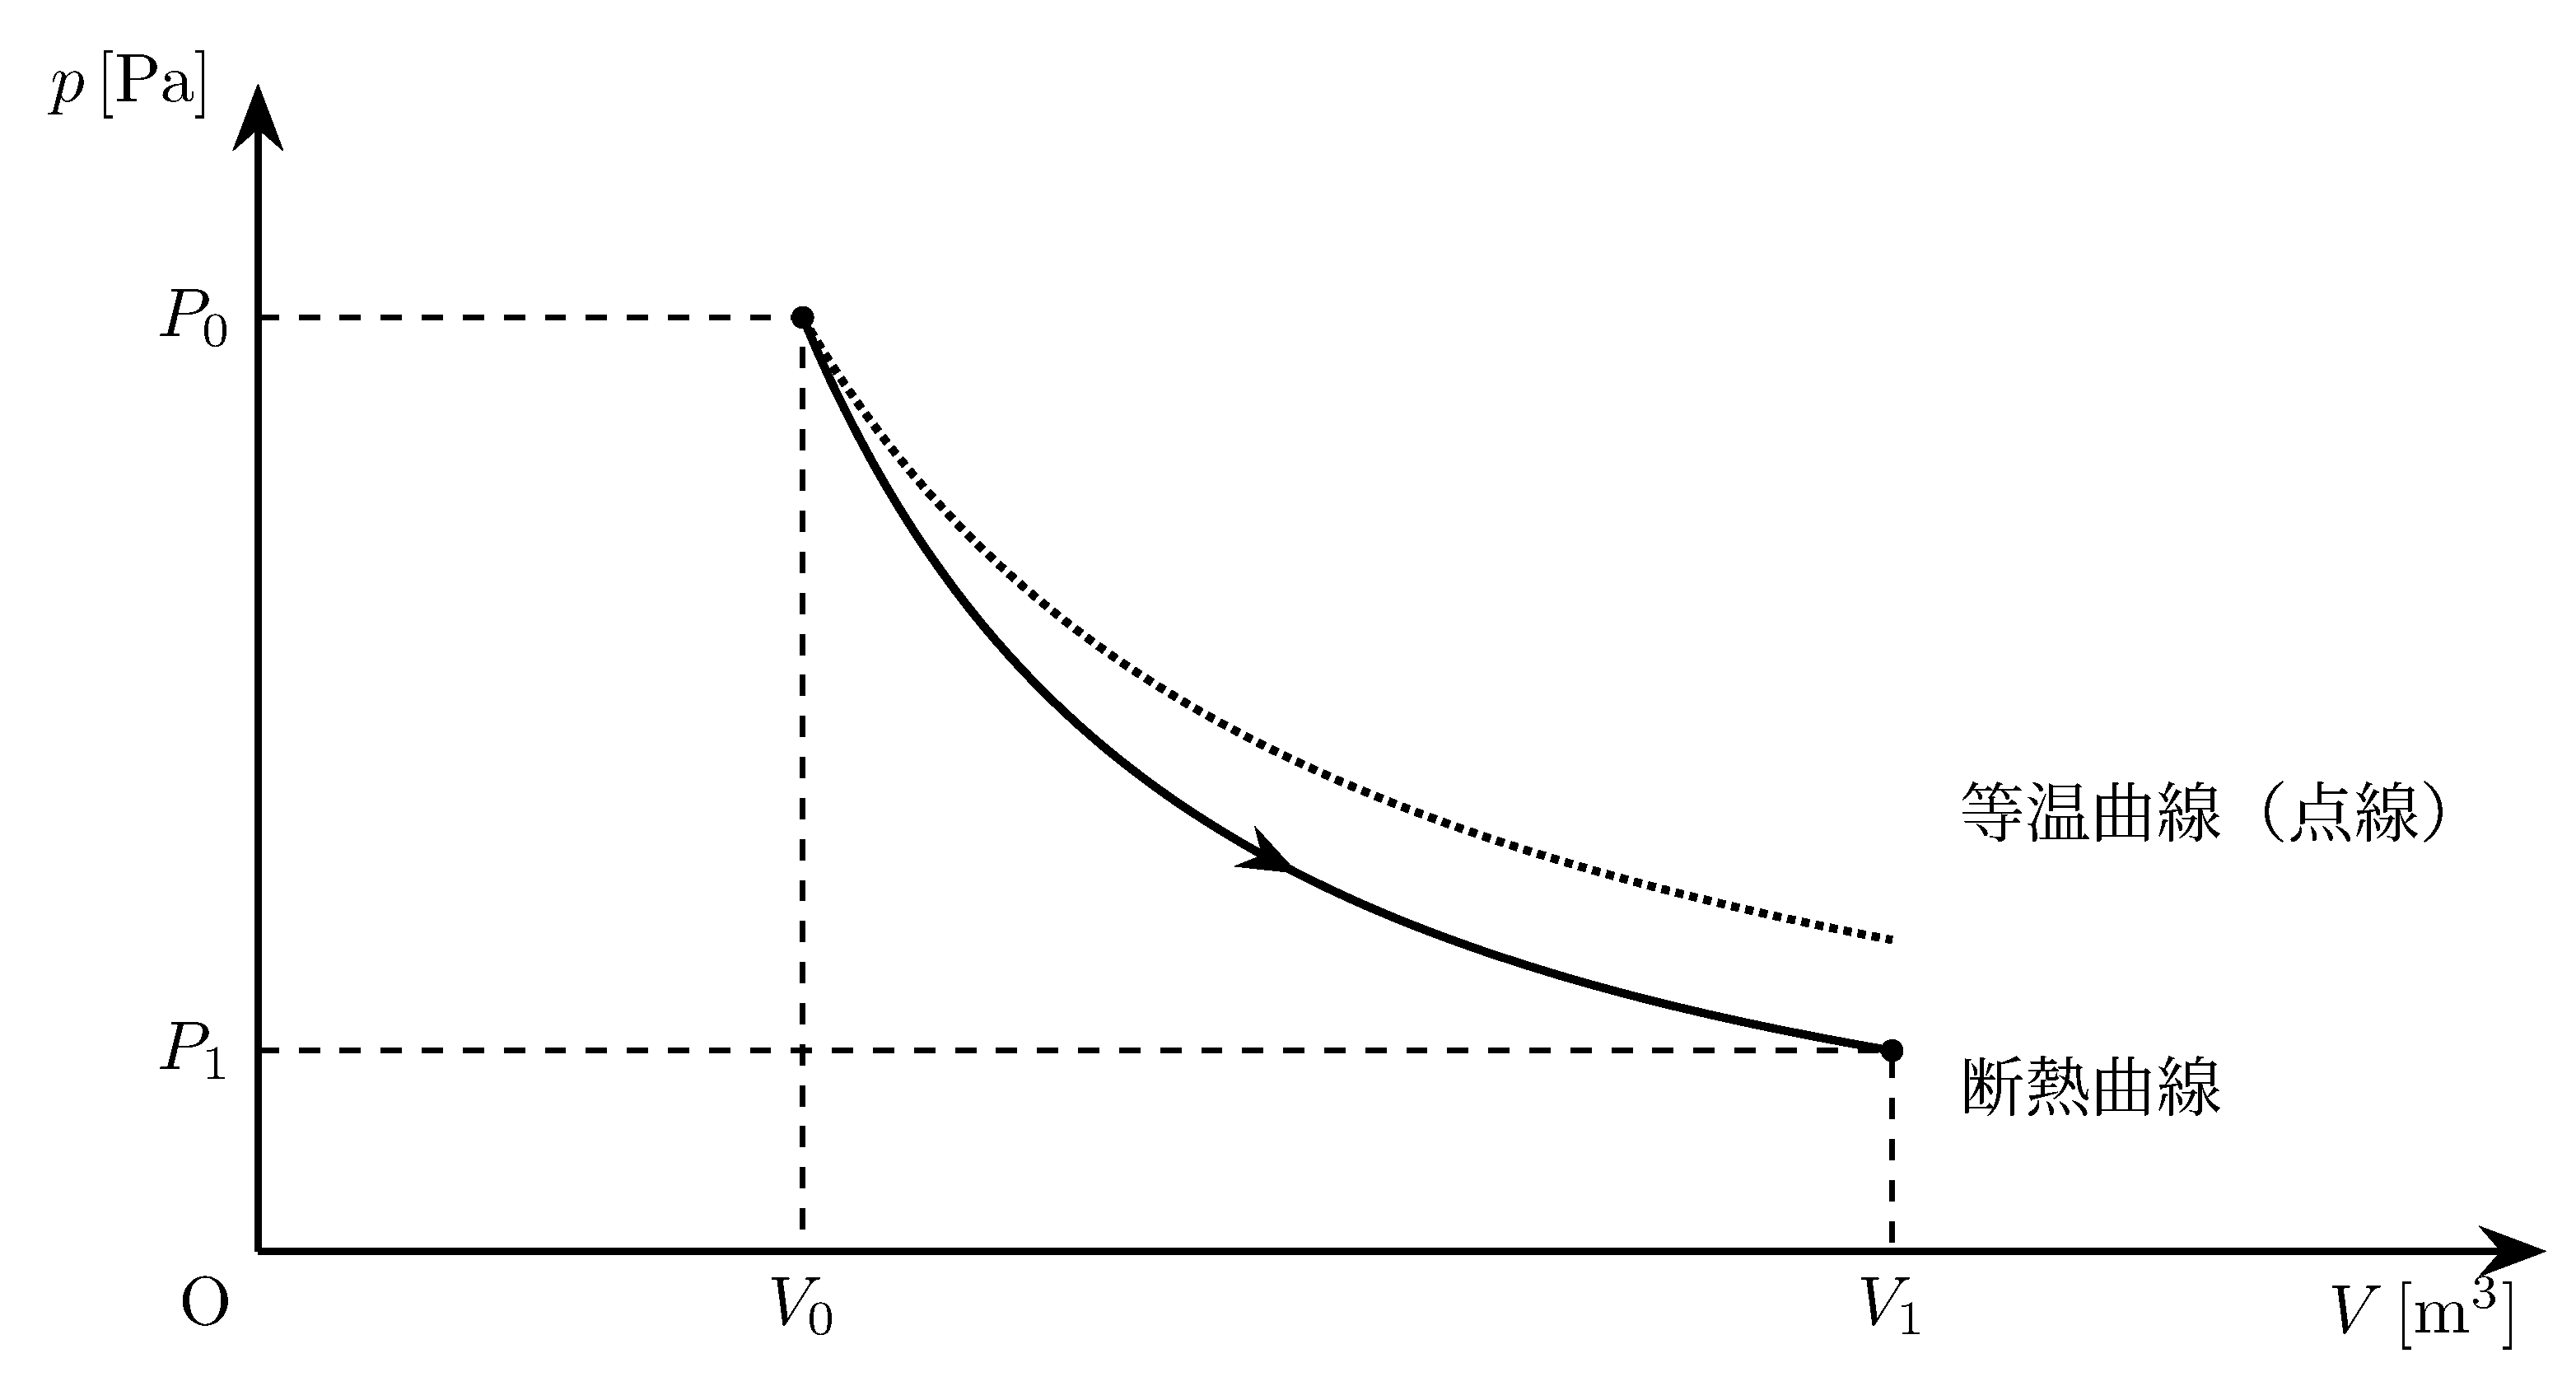
\includegraphics[keepaspectratio,width=106mm]{fig/ch17_ex13_pv.png}
       \fi
       \end{center}
       \hspace*{\fill}\Ans
\ko{3} 内部エネルギーは絶対温度だけで決まるので，
       \[\Delta U=nC_V(T_1-T_0)\U{J}\Ans\]
       $T_1<T_0$であるから$\Delta U<0$，すなわち内部エネルギーは減少する．
\ko{4} 断熱変化であるから$Q=0$であり，熱力学第一法則$Q=\Delta U+w$より，
       \[w=-\Delta U=nC_V(T_0-T_1)\U{J}\Ans\]
\ko{5} $\gamma-1=\dfrac{R}{C_V}$である．ポアソンの式\mbox{$TV^{\gamma-1}=（一定）$}を始状態と終状態に適用して，
       \[T_0V_0^{\gamma-1}=T_1V_1^{\gamma-1}\]
       これを$V_1$について解くと，
       \Ana{V_1=V_0\left(\frac{T_0}{T_1}\right)^{\frac{1}{\gamma-1}}
             =V_0\left(\frac{T_0}{T_1}\right)^{\frac{C_V}{R}}\U{m^3}\Ans}
       $T_0>T_1$であるから$V_1>V_0$となり，膨張していることが確かめられる．
\end{komon}
\end{kaitou}
\end{reidaiunit}


\subsection{自由膨張}

次の例題のように，気体が真空中に拡散していく際には，左右の部屋の圧力が異なる状態を経て気体が真空側へと流れていき，最終的には両方の部屋の気体の圧力が等しくなったところで気体の流れが止まる．
このような真空中への気体の膨張を{\gtfamily 自由膨張}といい，特に熱を遮断した状態で真空中へ膨張させることを{\gtfamily 断熱自由膨張}という．

% 加筆（2026-09-21）：原本は「もともと気体の入っていた部屋から気体が出ていき，片方の部屋に
%   注目するとモル数が変化していくため」という説明だったが，ポアソンが使えない本当の理由は
%   「準静的過程でなく，気体全体に1つの圧力を定められない」ことである（原本も練習［29］の
%   参考ではそう説明している）．23.1 で準静的過程を定義したので，ここで対比させた．
断熱自由膨張は，ここまで扱ってきた状態変化と違って{\gtfamily 準静的過程ではない}．
変化の途中では気体が一様でなく，出ていく側の部屋の方が密度も圧力も高いので，気体全体に対して1つの圧力$P$を定めることができない．
ポアソンの式は気体全体に対する状態方程式を用いて導いたものだから，断熱変化ではあるが，\,\AnaB{$PV^\gamma=（一定）$}\,を用いて考えてはいけない．

\begin{center}
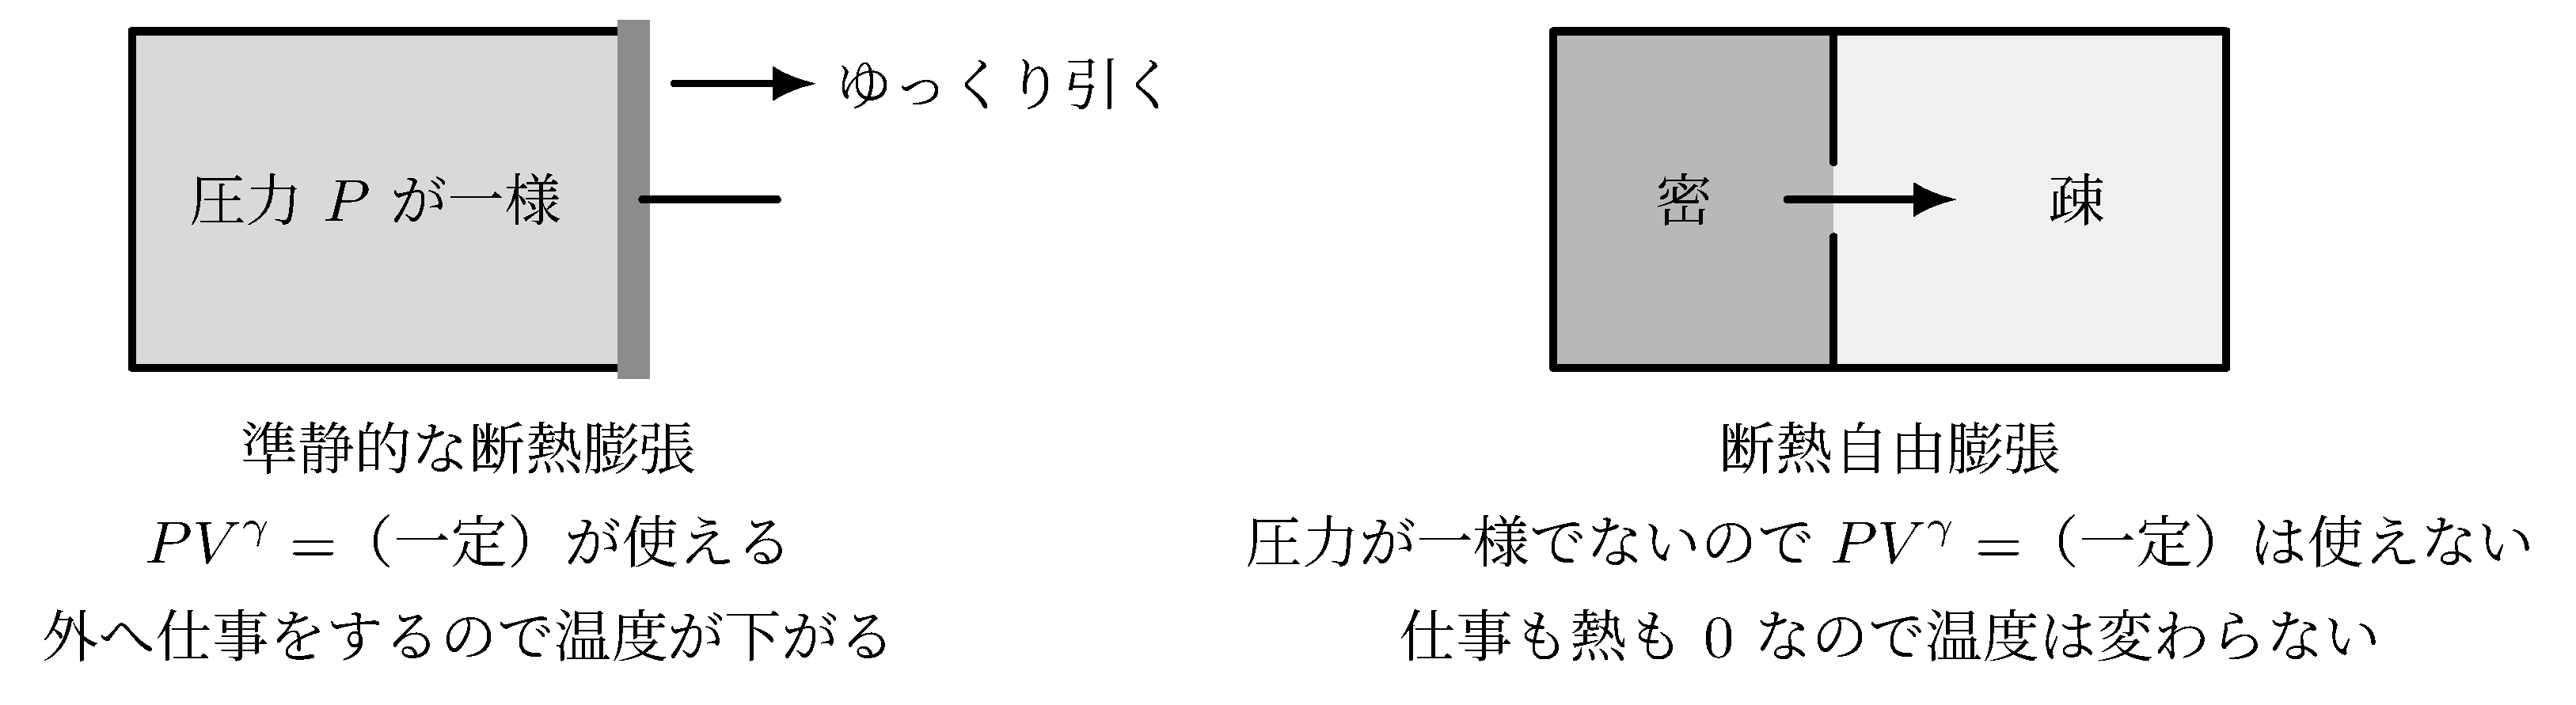
\includegraphics[keepaspectratio,width=132mm]{fig/n23_zu_jiyuu.png}
\end{center}

ではどう考えるか．
このような場合は{\gtfamily 箱全体を一つの系とみなして熱力学第一法則を適用する．}
箱全体の体積は変わらないので気体は外界に対して仕事をせず（$W_{\mathrm{out}}=0$），また断熱されているので箱の内外で熱のやりとりもない（$Q_{\mathrm{in}}=0$）．
よって箱内部の内部エネルギー変化が$\Delta U=0$となり，{\gtfamily 温度が変化しない}ことがわかる．

\bsNeed{40mm}
\begin{matome}{断熱自由膨張}
 \hspace{3mm} 熱を遮断した状態で真空中へ理想気体を膨張させるときは，{\gtfamily 箱全体}に対して熱力学第一法則を考える．\\[1mm]
 \hspace{3mm} $Q_{\mathrm{in}}=0$，$W_{\mathrm{out}}=0$\hspace{4mm} よって\hspace{4mm} $\Delta U=0$，すなわち\,\AnaB{温度は変わらない}．\\[1mm]
 \hspace{3mm} 準静的過程ではないので，{\gtfamily ポアソンの式$PV^\gamma=（一定）$を使ってはならない}．
\end{matome}

%%%%%%%%%%  例題14（23.4 のまとめ枠の直後。原本の【例題14】）  %%%%%%%%%%%%%%%%%%%%
\bsNeed{100mm}
\begin{reidaiunit}
\begin{reidai}{断熱自由膨張}
\begin{zuright}{52mm}
\hspace{1zw}断熱材で作られた容器の中に，仕切板を隔てて図の左側の空間にのみ定積モル比熱が$C_V\U{J/mol\cdot K}$，温度が$T_0\U{K}$の理想気体が$n\U{mol}$封入されている．
\zusep
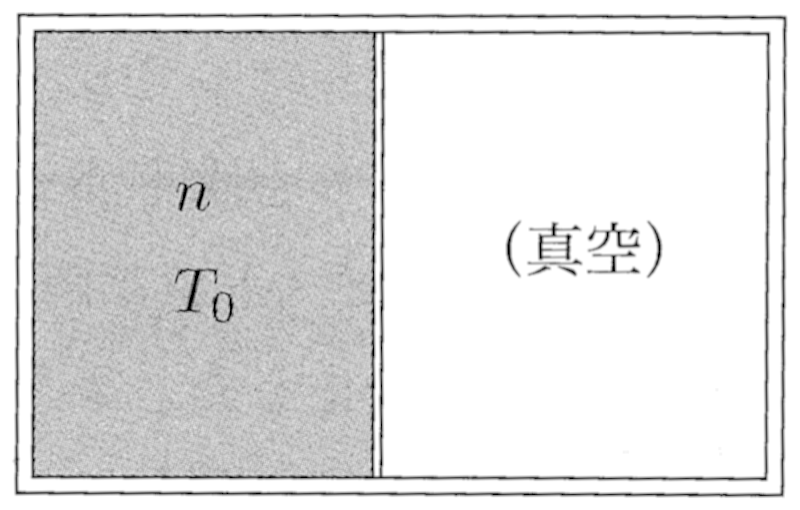
\includegraphics[keepaspectratio,width=52mm]{fig/ch17_ex14_box1.png}
\end{zuright}
\begin{komon}
\ko{1} この仕切板に穴を開けると気体は右側へと拡散していく．十分時間がたったのちの気体の温度$T^\prime\U{K}$を求めよ．
\end{komon}
\begin{zuright}{52mm}
\hspace{1zw}先と同じく断熱材で作られた容器の中に，仕切板を隔てて図のように左側，右側それぞれに異なる気体を封入する．左側（体積$V_1\U{m^3}$）には定積モル比熱$C_{V1}\U{J/mol\cdot K}$，温度が$T_1\U{K}$の理想気体が$n_1\U{mol}$だけ封入されており，右側（体積$V_2\U{m^3}$）には定積モル比熱$C_{V2}\U{J/mol\cdot K}$，温度が$T_2\U{K}$の理想気体が$n_2\U{mol}$だけ封入されている．
\zusep
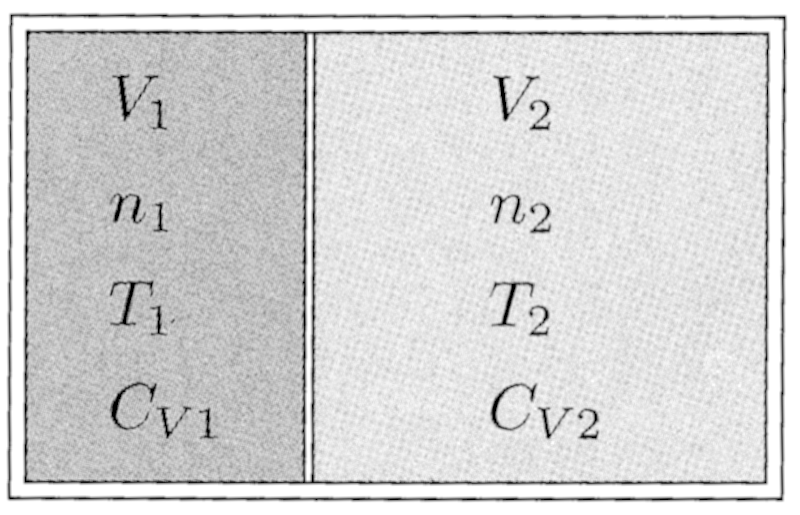
\includegraphics[keepaspectratio,width=52mm]{fig/ch17_ex14_box2.png}
\end{zuright}
\begin{komon}
\ko{2} この仕切板を取り外し，外界との熱のやり取りを断って2つの気体を混合する．十分時間がたったのちの温度$T\U{K}$を求めよ．
\end{komon}
\end{reidai}

\begin{sisinE}
どちらも{\gtfamily 容器全体を一つの系とみなして熱力学第一法則を立てる}．容器の体積は変わらないので外界と仕事のやり取りはなく（$W_{\mathrm{out}}=0$），断熱材で作られているので熱のやり取りもない（$Q_{\mathrm{in}}=0$）．したがって容器全体の内部エネルギーの変化は$\Delta U=0$である．

(2)では，容器全体の内部エネルギー変化は左側の気体の変化と右側の気体の変化の和であることを使う．
\end{sisinE}

\Key{真空中への断熱自由膨張 $\Rightarrow$ 箱全体に対しての熱力学第一法則}

\begin{kaitou}
\begin{komon}
\ko{1} 容器全体を一つの系とみなすと，体積が変わらないので$W_{\mathrm{out}}=0$，断熱材なので$Q_{\mathrm{in}}=0$である．よって熱力学第一法則より
       \[\Delta U=Q_{\mathrm{in}}-W_{\mathrm{out}}=0\]
       一方，内部エネルギーの変化は$\Delta U=nC_V(T^\prime-T_0)$と表せるから，$nC_V\neq 0$より$T^\prime-T_0=0$，すなわち
       \[T^\prime=T_0\U{K}\Ans\]
\ko{2} こちらも容器全体では$Q_{\mathrm{in}}=0$, $W_{\mathrm{out}}=0$であるから$\Delta U=0$である．混合後の温度を$T\U{K}$とすると，左側の気体の内部エネルギー変化と右側の気体の内部エネルギー変化の和が$\Delta U$であるから，
       \[n_1C_{V1}(T-T_1)+n_2C_{V2}(T-T_2)=0\]
       これを$T$について解いて，
       \Ana{T=\frac{n_1C_{V1}T_1+n_2C_{V2}T_2}{n_1C_{V1}+n_2C_{V2}}\U{K}\Ans}
\end{komon}
\end{kaitou}
\end{reidaiunit}


\subsection{熱機関と熱効率}

% 訂正（2026-09-21 レビュー）：原本は「最初の状態に戻る過程を熱機関，または熱サイクルと呼ぶ」
%   だが，本節の後半で反時計回りのサイクルを冷蔵庫・ヒートポンプとして扱っており，
%   「サイクル＝熱機関」では教材内で食い違う．2つを分けて定義する．
いくつかの状態変化を組み合わせ，最初の状態に戻るような一連の過程を{\gtfamily 熱サイクル}（循環過程）という．
そのうち，{\gtfamily 高温の物体から熱を受け取り，1周ごとに正味の仕事を外界へ取り出す装置}を{\gtfamily 熱機関}という．
蒸気機関や自動車のエンジンがこれにあたる．
（同じサイクルでも逆向きに回せば，仕事を受け取って熱を運ぶ装置になる．これは熱機関ではなく冷蔵庫やヒートポンプで，本節の最後に述べる．）

% 加筆（2026-09-21）：なぜ元の状態に戻す必要があるのか／なぜ熱を捨てねばならないのかは，
%   原本では練習［31］の【参考】（蒸気機関車の説明）にしか書かれていなかった．
%   本文に上げ，第21回 21.5（熱力学第二法則）と結んだ．
\Kou{1}{なぜ「元の状態に戻す」のか}

石炭をくべて高温の熱源を作っただけでは機関車は進まない．
もらった熱を，車輪を回すという{\gtfamily 力学的な仕事}に変換しなければならない．
そこで気体を用いるのだが，ただ膨張させて仕事をさせるだけだと，膨張しきったところで「やりっぱなし」の状態になり，それ以上仕事を続けられない．
そこで気体を元の状態に戻し，何度でも仕事ができるようにする．

ところがこの「元に戻す」過程で，気体はどうしても外に熱を捨てなければならない．
第21回 21.5 で述べた{\gtfamily 熱力学第二法則}（一つの熱源から熱を取り出し，それをすべて仕事に変えて，ほかに何の変化も残さないようにすることはできない）がこれである．
しかも熱は高温側から低温側にしか流れないので，捨てる相手は熱をもらった高温の熱源ではありえない．
熱をもらう側を{\gtfamily 高熱源}，捨てる側を{\gtfamily 低熱源}（蒸気機関車でいえば外気）と呼ぶ．

\begin{center}
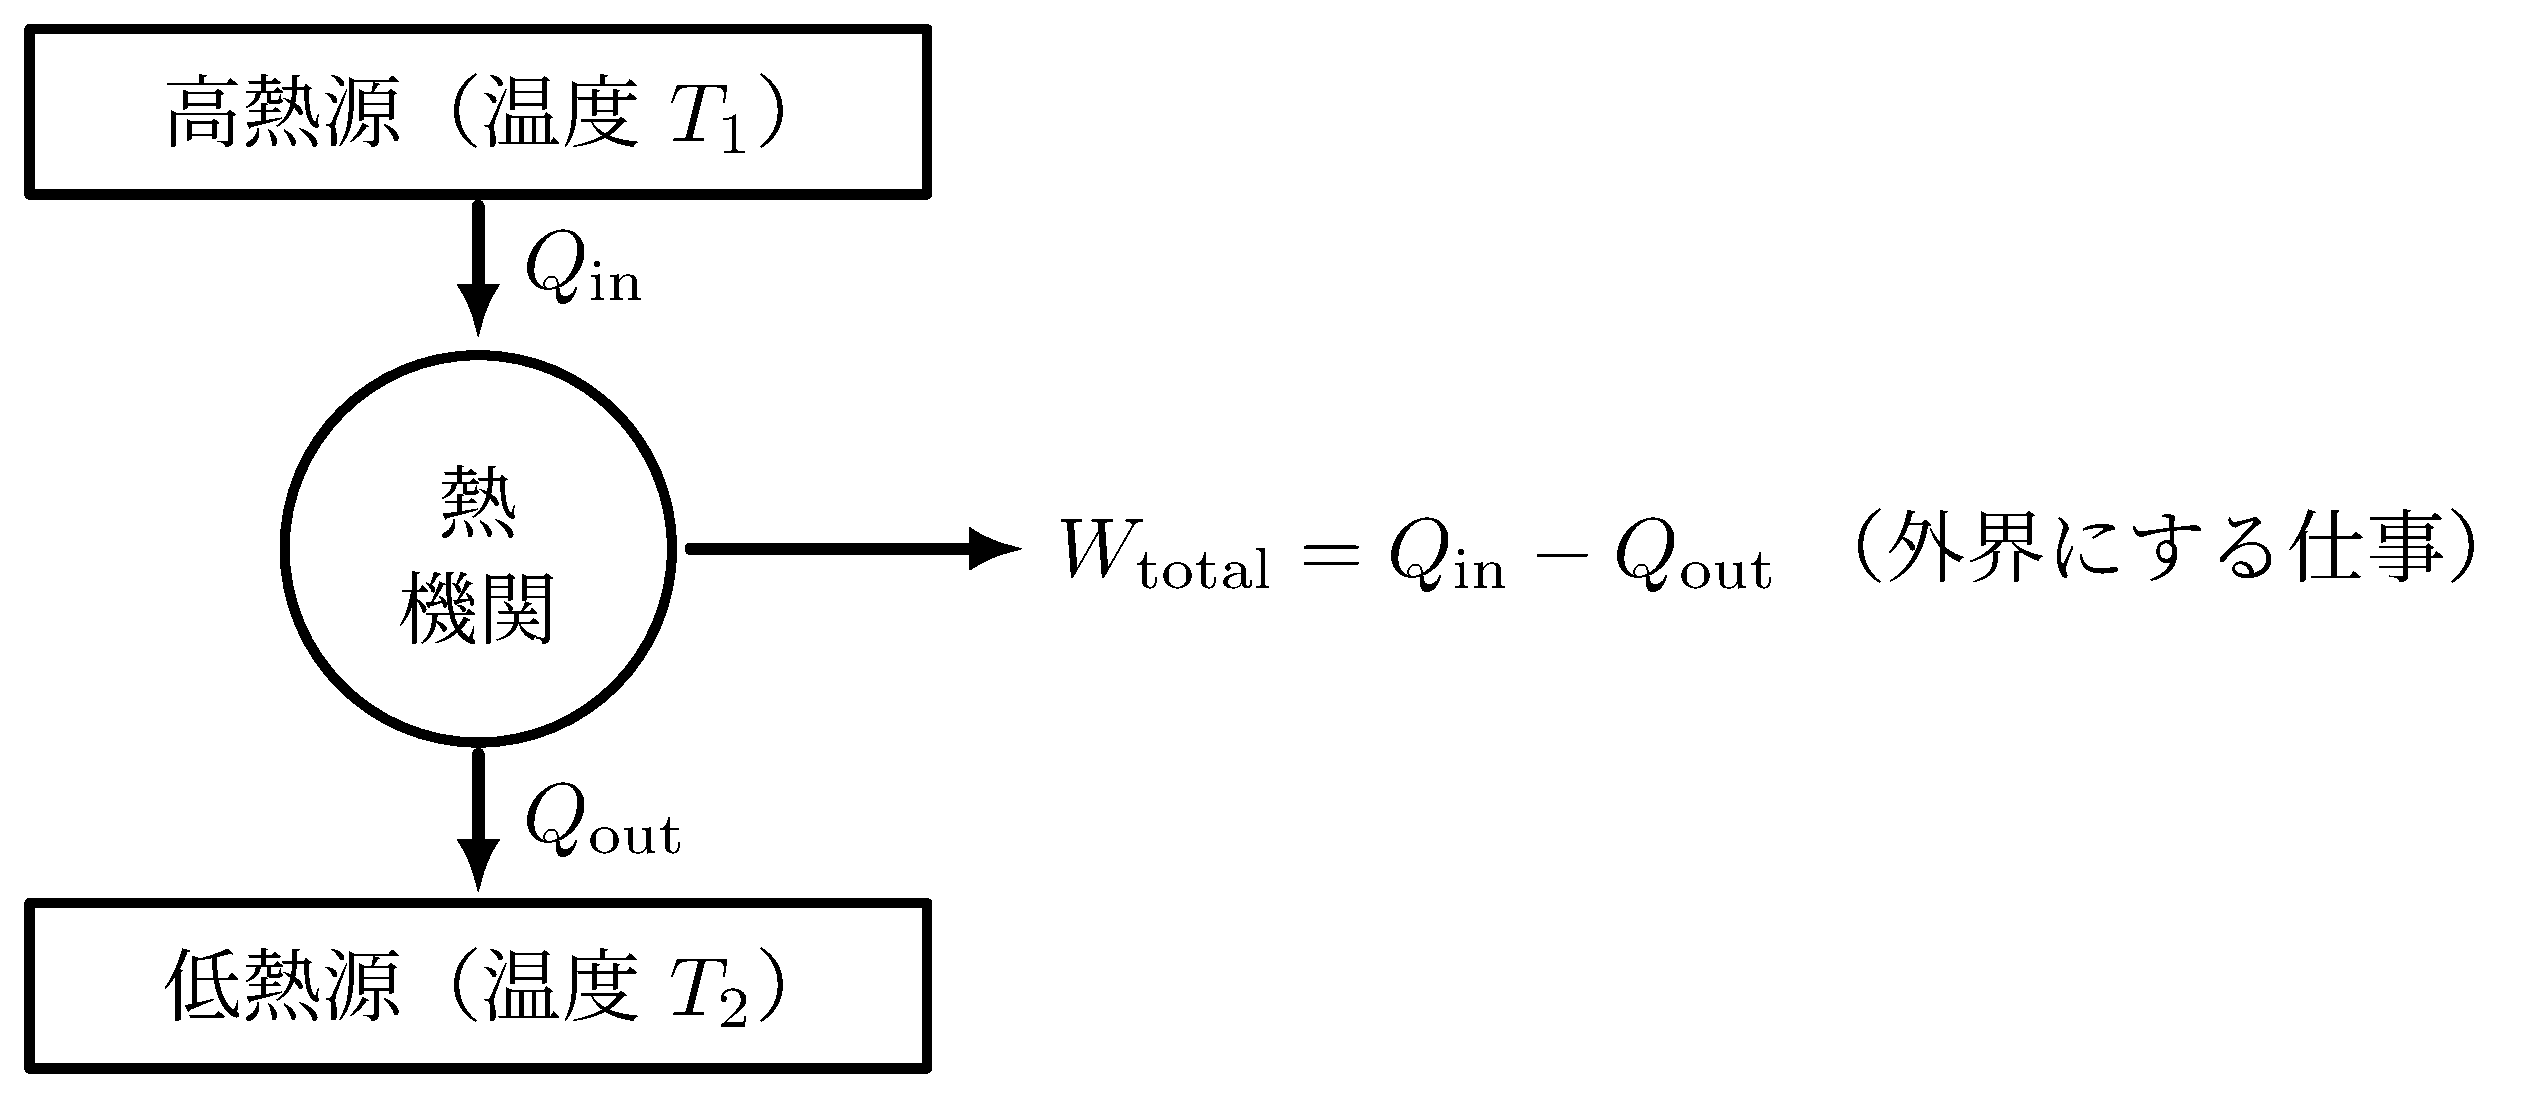
\includegraphics[keepaspectratio,width=98mm]{fig/n23_zu_netu.png}
\end{center}

\Kou{2}{熱効率}

サイクルを1周すると最初の状態に戻るので，トータルでは温度変化がなく，内部エネルギーの変化量は$\Delta U=0\U{J}$である．
1周の間に，吸熱過程で受け取った熱量の合計を$Q_{\mathrm{in}}\U{J}$，放熱過程で捨てた熱量の合計を$Q_{\mathrm{out}}\U{J}$（どちらも正の量とする）とすれば，サイクル全体に対する熱力学第一法則より，1周で気体が外界にする仕事の合計$W_{\mathrm{total}}\U{J}$は
\AnaBD{Q_{\mathrm{in}}-Q_{\mathrm{out}}=\Delta U+W_{\mathrm{total}}=W_{\mathrm{total}}}
と表せる．
これは，$Q_{\mathrm{in}}\U{J}$の熱を与え，そのうち$W_{\mathrm{total}}\U{J}$分だけ仕事をし，余りのエネルギー$Q_{\mathrm{out}}\U{J}$を熱として捨てている，と解釈できる．

% 加筆（2026-09-21 レビュー）：1周で ΔU=0 なのに Q も W も 0 でない理由。
1周すると$\Delta U=0$になるのは，内部エネルギーが{\gtfamily 状態が決まれば決まる量}（圧力・体積・温度が決まれば値が決まる）だからである．
これに対し$Q_{\mathrm{in}}$や$W_{\mathrm{out}}$は{\gtfamily どんな経路をたどったかで決まる量}なので，元の状態に戻っても$0$にはならない．
熱機関はこの違いを使って，熱からくり返し仕事を取り出している．

このときの{\gtfamily 加えた熱量に対してどれだけの仕事をするか}を{\gtfamily 熱効率}と呼び，熱効率$e$は
\AnaBD{e=\dfrac{W_{\mathrm{total}}}{Q_{\mathrm{in}}}=1-\dfrac{Q_{\mathrm{out}}}{Q_{\mathrm{in}}}}
となる．
上で述べたように$Q_{\mathrm{out}}$を$0$にすることはできないので，つねに$0\leqq e<1$であり，{\gtfamily 熱効率が$1$（＝100\%）になる熱機関は存在しない}．

\Kou{3}{$P$-$V$図の囲む面積}

また，各過程での$P$-$V$図における符号付き面積を考えることで，仕事の合計$W_{\mathrm{total}}\U{J}$は{\gtfamily 熱機関の各過程で囲まれた部分の符号付き面積}として表すことができる．

\begin{center}
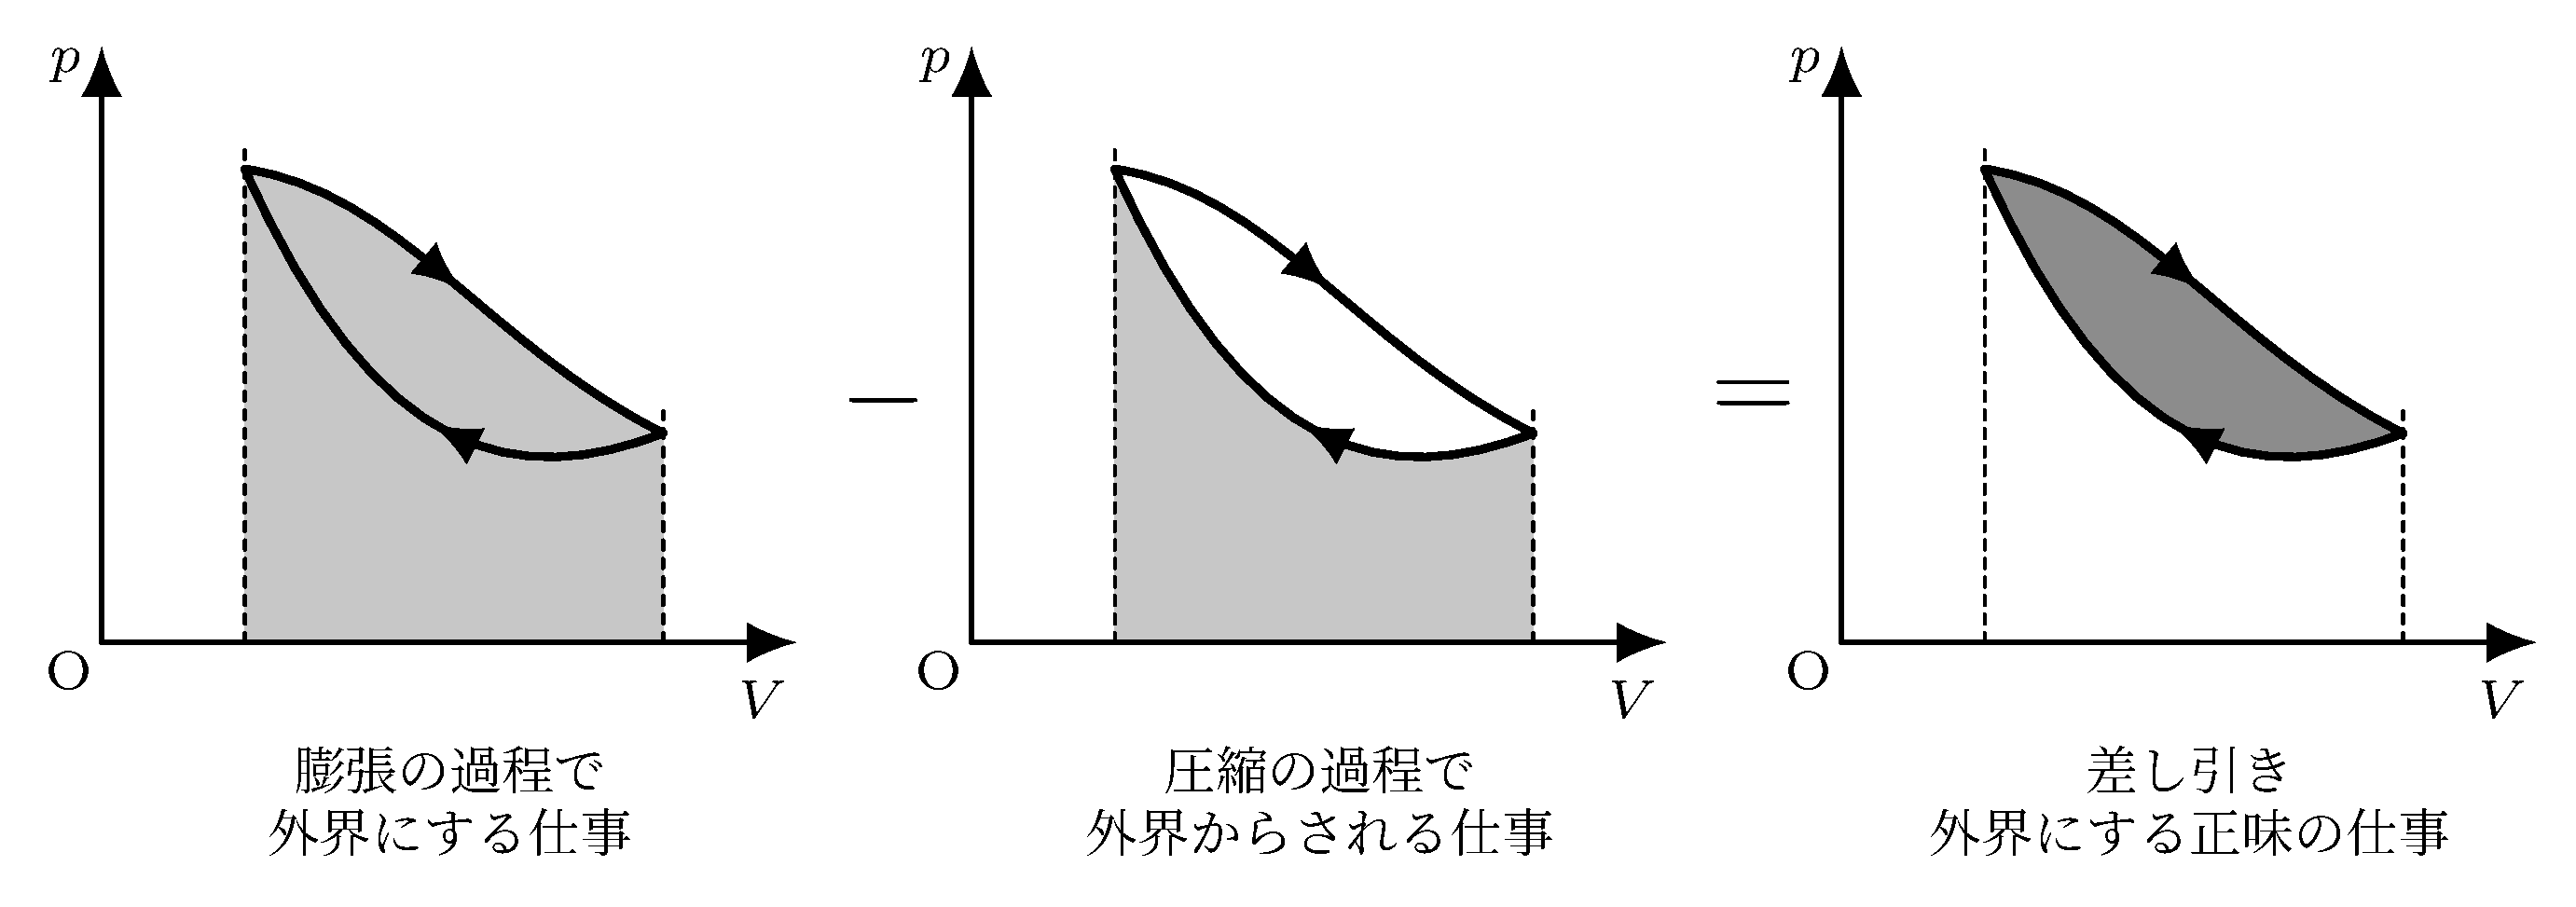
\includegraphics[keepaspectratio,width=150mm]{fig/n23_zu_cycle.png}
\end{center}

このとき，\,\AnaB{時計回り}\,に回る熱機関ならば$W_{\mathrm{total}}>0$となって囲む面積と等しいが，{\gtfamily 反時計回り}に回る場合は$W_{\mathrm{total}}<0$となり，面積に$-1$をかけた値となる．
反時計回りのサイクルは，外から仕事をしてもらって低温側から高温側へ熱を汲み上げる装置，すなわち冷蔵庫やヒートポンプにあたる．

% 加筆（2026-09-21）：熱機関には原本の例題が無いので，解き方の手順をまとめ枠にした．
%   練習［31］［32］がそのままこの手順である．
\bsNeed{56mm}
\begin{matome}{熱機関（熱サイクル）の解き方}
 \hspace{3mm} \MARU{1}\hspace{2mm} 各点$\mathrm{A}$, $\mathrm{B}$, $\cdots$について状態方程式を立て，圧力・体積・温度を出す\\[0.5mm]
 \hspace{3mm} \MARU{2}\hspace{2mm} 各過程について$W_{\mathrm{out}}$（$P$-$V$図の面積）と$\Delta U=nC_V\Delta T$を求め，\\
 \hspace{10mm} 熱力学第一法則$Q_{\mathrm{in}}=\Delta U+W_{\mathrm{out}}$から吸熱量を出す（表にまとめるとよい）\\[0.5mm]
 \hspace{3mm} \MARU{3}\hspace{2mm} $W_{\mathrm{total}}$は各過程の$W_{\mathrm{out}}$の総和（符号込み）＝サイクルが囲む符号付き面積\\[0.5mm]
 \hspace{3mm} \MARU{4}\hspace{2mm} $Q_{\mathrm{in}}$には{\gtfamily 正の（吸熱の）過程だけ}を足す．負の過程は放熱で$Q_{\mathrm{out}}$側\\[1mm]
 \hspace{3mm} 検算：1周すると$\Delta U=0$だから，各過程の$\Delta U$の総和は必ず$0$になる
\end{matome}

% 加筆（2026-09-21 レビュー）：熱機関は本回の総合問題なのに，ここまで例題が1つも無く
%   いきなり練習［31］［32］だった．手順をなぞる小さな例をひとつ本文に置く。
%   三角形サイクルにしたのは，長方形（［31］）・等温入り（［32］）と重ならないため。
%   数値は，斜めの過程 B→C が途中でも吸熱のままになるように選んである
%   （直線の過程は終盤で放熱に転じることがあるので，値の取り方に注意）。
% 見出し＋問題設定だけが前ページに残ると，本文の「右下の図」が次ページになってしまう
\bsNeed{120mm}
\Kou{4}{手順の確認}

単原子分子理想気体（$C_V=\dfrac{3}{2}R$）$n\U{mol}$を，右下の図の$\mathrm{A}\rightarrow\mathrm{B}\rightarrow\mathrm{C}\rightarrow\mathrm{A}$の順に一周させる．
$\mathrm{A}$の圧力・体積・温度を$P_0$, $V_0$, $T_0$とし，$\mathrm{A}\rightarrow\mathrm{B}$は定積，$\mathrm{B}\rightarrow\mathrm{C}$は$P$-$V$図で直線，$\mathrm{C}\rightarrow\mathrm{A}$は定圧である．

\begin{zuright}{88mm}
\hspace{1zw}\MARU{1}\ 各点の温度を出す．$P_0V_0=nRT_0$であるから，状態方程式より
\[\mathrm{B}:2P_0\cdot V_0=nRT_{\mathrm{B}}\ \Rightarrow\ T_{\mathrm{B}}=2T_0\]
\[\mathrm{C}:P_0\cdot 3V_0=nRT_{\mathrm{C}}\ \Rightarrow\ T_{\mathrm{C}}=3T_0\]
\hspace{1zw}\MARU{2}\ 各過程の$W_{\mathrm{out}}$は$P$-$V$図の面積，$\Delta U$は$nC_V\Delta T=\dfrac{3}{2}nR\Delta T$である．
$nR=\dfrac{P_0V_0}{T_0}$を使って$P_0V_0$を単位に書くと次の表になる．
\zusep
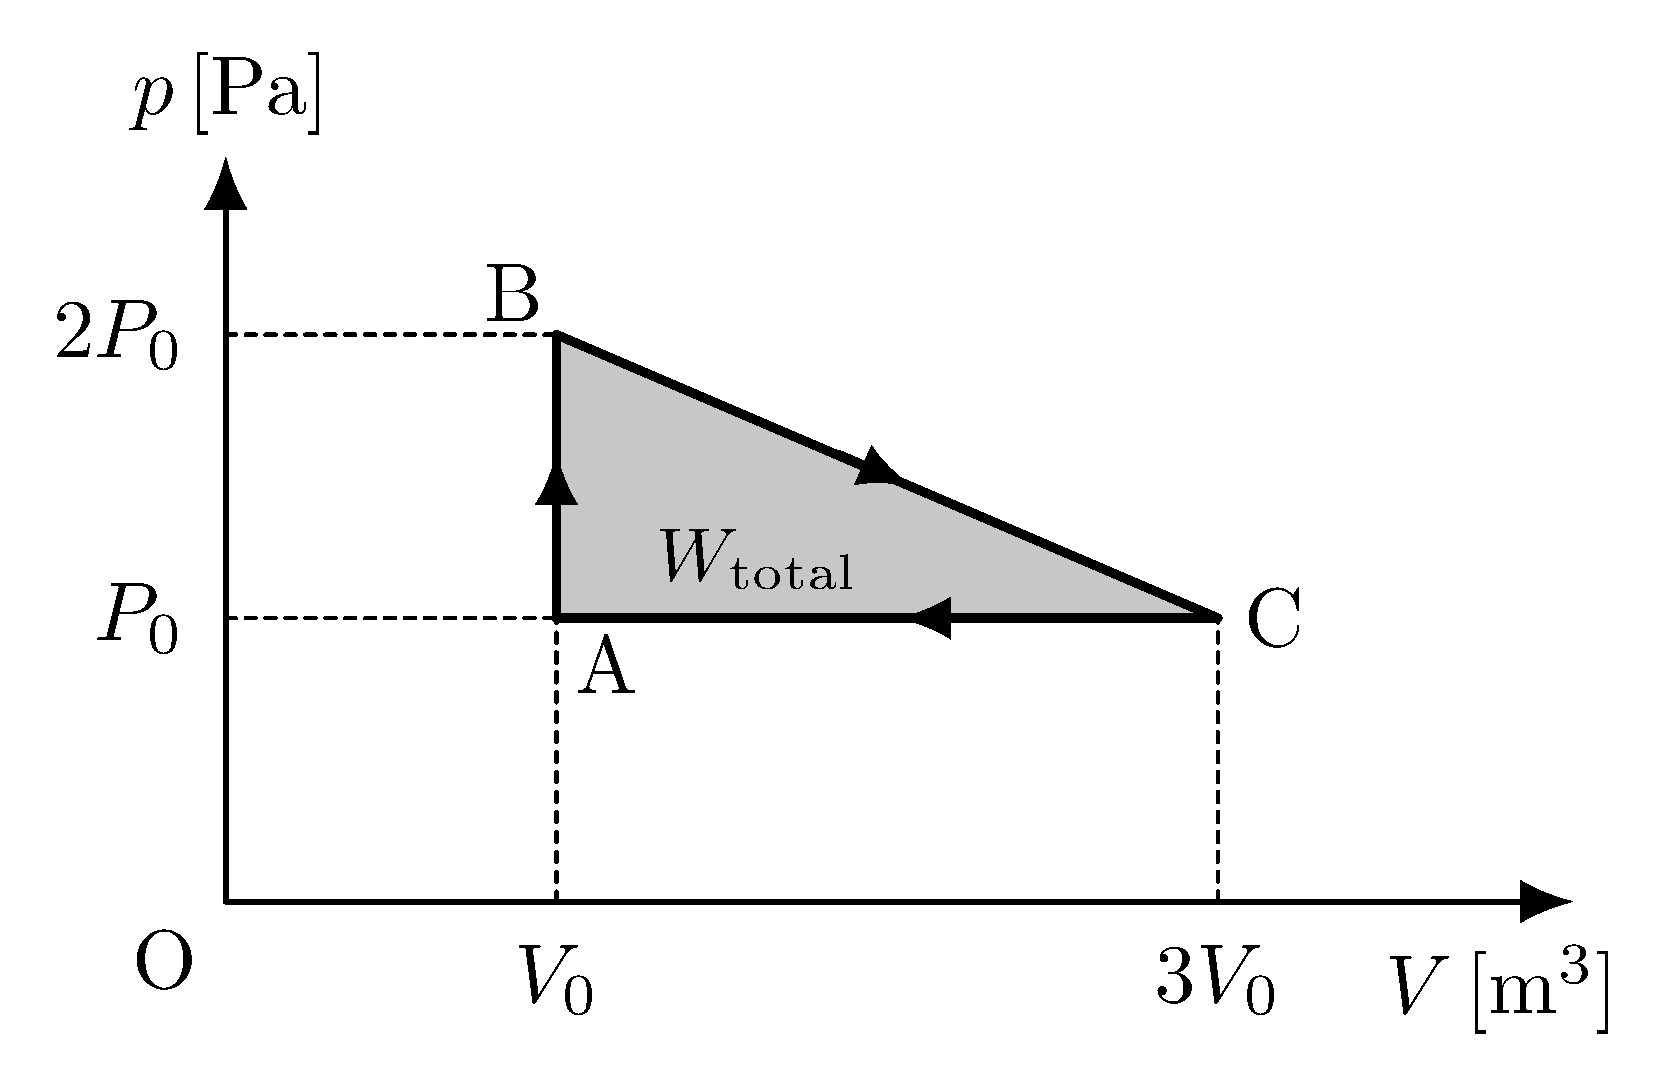
\includegraphics[keepaspectratio,width=88mm]{fig/n23_zu_rei.png}
\end{zuright}

\begin{center}
\begin{tabular}{l@{\hspace{7mm}}c@{\hspace{7mm}}c@{\hspace{7mm}}c@{\hspace{7mm}}l}
過程 & $W_{\mathrm{out}}$ & $\Delta U$ & $Q_{\mathrm{in}}=\Delta U+W_{\mathrm{out}}$ & \\ \hline
$\mathrm{A}\rightarrow\mathrm{B}$（定積） & $0$ & $\frac{3}{2}P_0V_0$ & $\frac{3}{2}P_0V_0$ & 吸熱\\
$\mathrm{B}\rightarrow\mathrm{C}$（直線） & $3P_0V_0$ & $\frac{3}{2}P_0V_0$ & $\frac{9}{2}P_0V_0$ & 吸熱\\
$\mathrm{C}\rightarrow\mathrm{A}$（定圧） & $-2P_0V_0$ & $-3P_0V_0$ & $-5P_0V_0$ & 放熱\\ \hline
合計 & $P_0V_0$ & $0$ & &
\end{tabular}
\end{center}

\noindent $\mathrm{B}\rightarrow\mathrm{C}$の$W_{\mathrm{out}}$は台形の面積$\frac{1}{2}(2P_0+P_0)(3V_0-V_0)=3P_0V_0$である．
$\Delta U$の列の合計が$0$になっているので，ここまでの計算は正しい（\MARU{2}の検算）．

\hspace{1zw}\MARU{3}\ 正味の仕事は$W_{\mathrm{out}}$の総和で$W_{\mathrm{total}}=P_0V_0\U{J}$．
これは三角形$\mathrm{ABC}$の面積$\frac{1}{2}\cdot 2V_0\cdot P_0=P_0V_0$と一致する．

\hspace{1zw}\MARU{4}\ 吸熱しているのは$\mathrm{A}\rightarrow\mathrm{B}$と$\mathrm{B}\rightarrow\mathrm{C}$だから，
\[Q_{\mathrm{in}}=\frac{3}{2}P_0V_0+\frac{9}{2}P_0V_0=6P_0V_0\U{J}\]
であり，熱効率は
\[e=\frac{W_{\mathrm{total}}}{Q_{\mathrm{in}}}=\frac{P_0V_0}{6P_0V_0}=\frac{1}{6}\fallingdotseq 0.17\]
となる．与えた熱の$17\%$しか仕事にならず，残りは捨てている，ということである．

この手順のまま，練習［31］［32］にあたること．


\newpage

%%%%%%%%%%%%%%%%%%%%  練習問題  %%%%%%%%%%%%%%%%%%%%
% 第22回の［21］に続く．章単体で組んだときも番号が本体と一致するように明示しておく
\setcounter{qno}{21}

\filbreak
\Rank{A問題}

% A問題の統合（再編案の「A2→1」）：旧⑯[17]（(1)(2)）と旧⑰[24]（比熱比）を1題にまとめた．
%   設問は1つも失われていない．
\Mon{基本事項の確認}

\hspace{1zw}以下の設問に答えよ．
\begin{komon}
\ko{1} 容器内の気体の圧力を$1.0\times 10^5\U{Pa}$に保ちながら，体積を$2.0\times 10^{-4}\U{m^3}$だけ増加させた．このとき気体が外界に対してした仕事は何$\U{J}$か．
\ko{2} 気体に$4.2\times 10^3\U{J}$の熱を加えたところ，気体は膨張し，ピストンに対して$2.4\times 10^3\U{J}$だけ仕事をした．このとき気体の内部エネルギーの増加は何$\U{J}$か．
\ko{3} 単原子分子理想気体，二原子分子理想気体の定積モル比熱はそれぞれ$\dfrac{3}{2}R$, $\dfrac{5}{2}R$である．このときそれぞれの比熱比$\gamma$はいくらか．
\end{komon}

\filbreak
\Rank{B問題}

\Mon[\Sitei]{気体がする仕事}

\hspace{1zw}一定量の理想気体の状態を以下の$p$-$V$図の矢印の向きに静かに変化させた．このとき気体が外界にした仕事$w\U{J}$をそれぞれ求め，$p_0\U{Pa}$, $p_1\U{Pa}$, $V_0\U{m^3}$, $V_1\U{m^3}$を用いて表せ．必要があれば積分公式$\displaystyle\int\frac{1}{x}dx=\log_e|x|+C$を用いよ．

\begin{center}
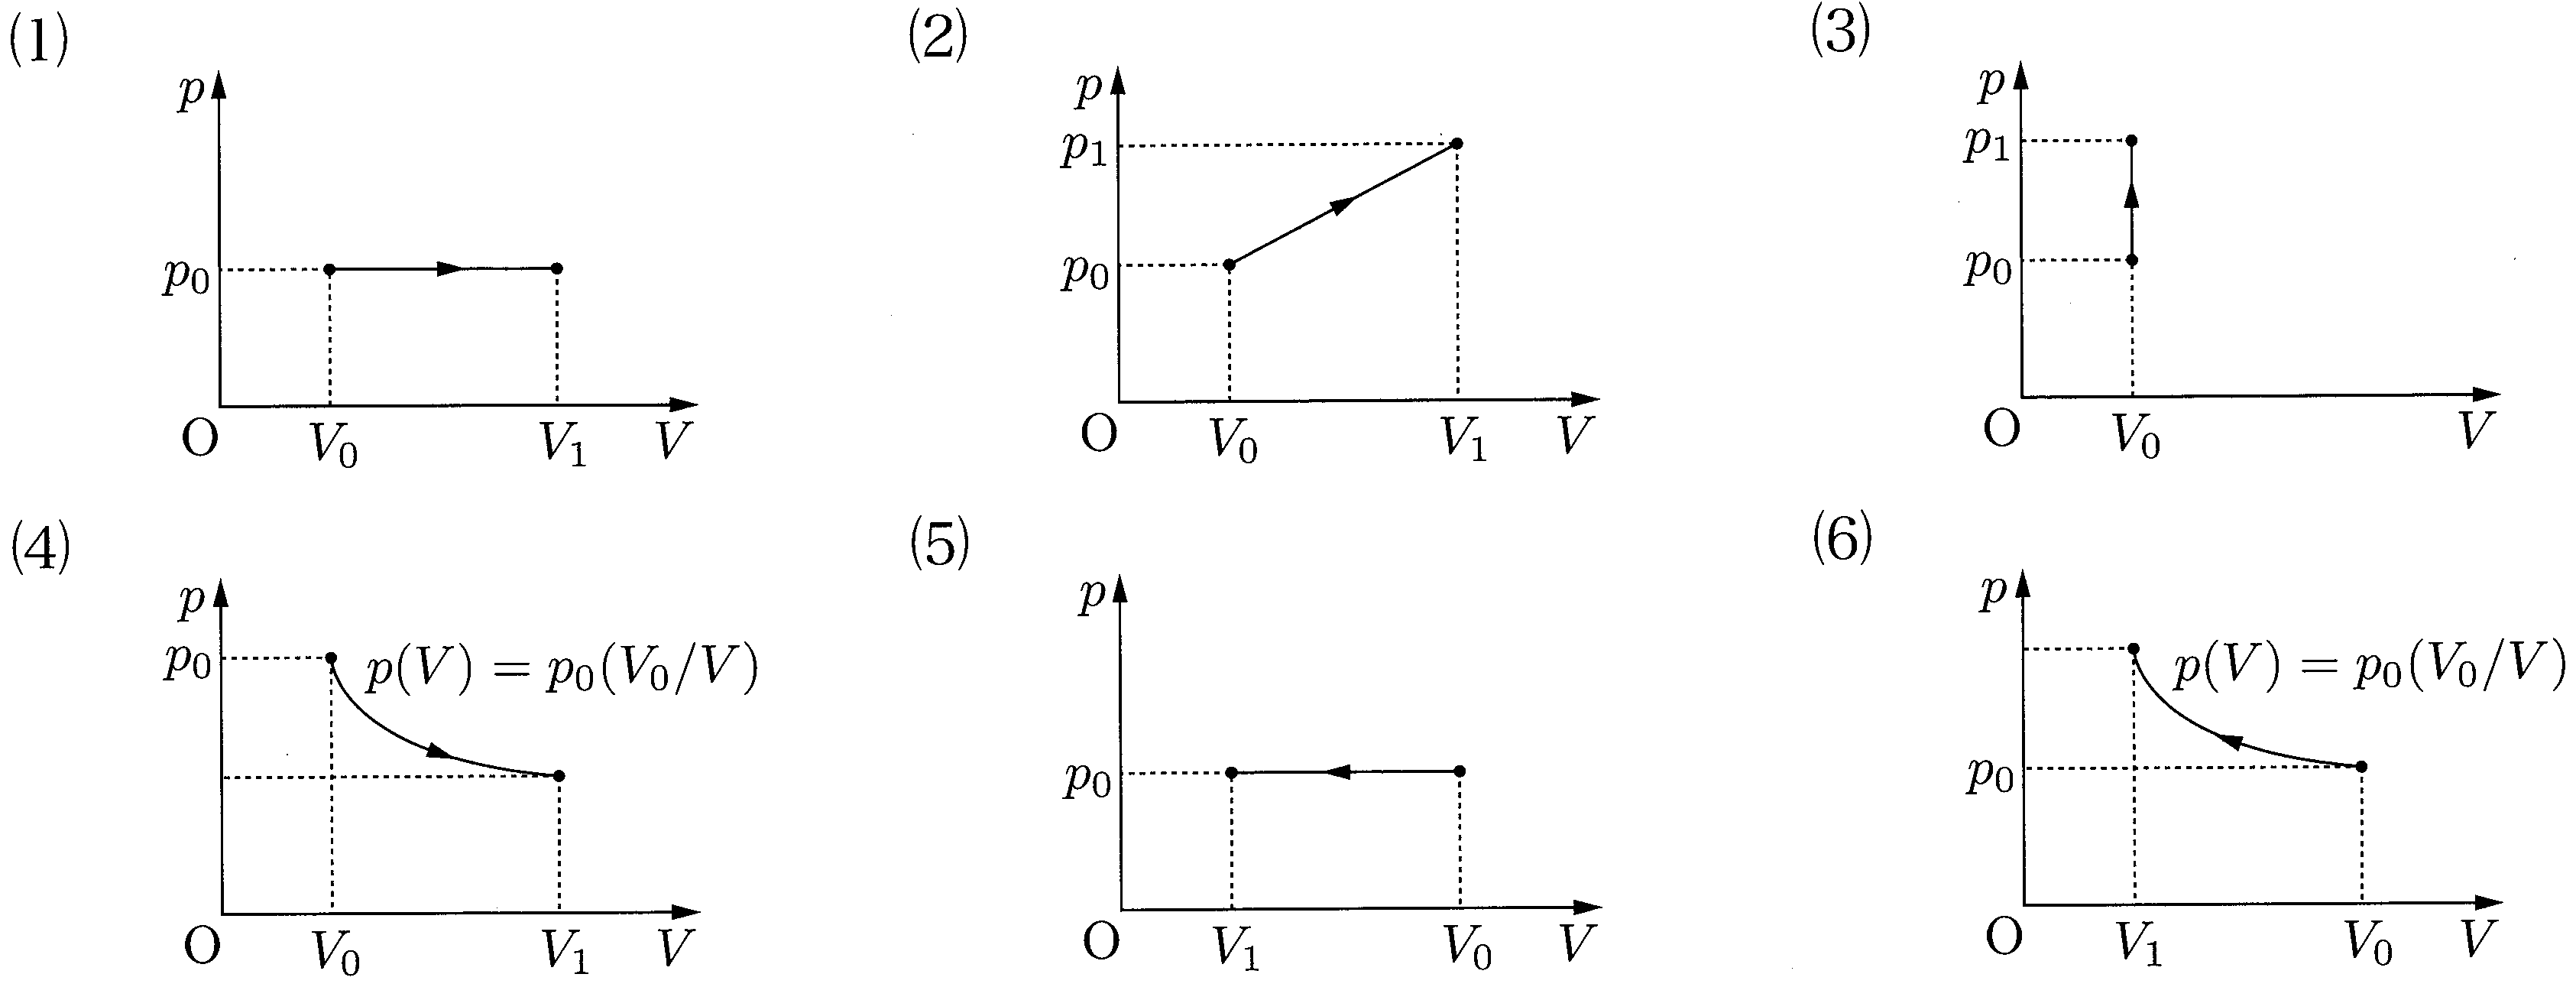
\includegraphics[keepaspectratio,width=148mm]{fig/ch16_p40_pv6.png}
\end{center}

\Mon[\Sitei]{鉛直シリンダー}

\begin{zuright}{28mm}
\hspace{1zw}右図のように鉛直に立ててある断面積$S\U{m^2}$のシリンダーの中に，質量$M\U{kg}$のなめらかに動くことのできるピストンで，定積モル比熱が$C_V\U{J/mol\cdot K}$の理想気体を$n\U{mol}$だけ封入した．初め，シリンダーの底からピストンまでの高さは$l_0\U{m}$であり，大気の圧力は$p_0\U{Pa}$であった．シリンダー内にはヒーターが取り付けられており，気体に対して熱を与えることができる．シリンダーおよびピストンは断熱材でできており，ヒーターによって与えた熱が外界に拡散することはないものとする．気体定数を$R\U{J/mol\cdot K}$，重力加速度の大きさを$g\U{m/s^2}$として以下の設問に答えよ．
\zusep
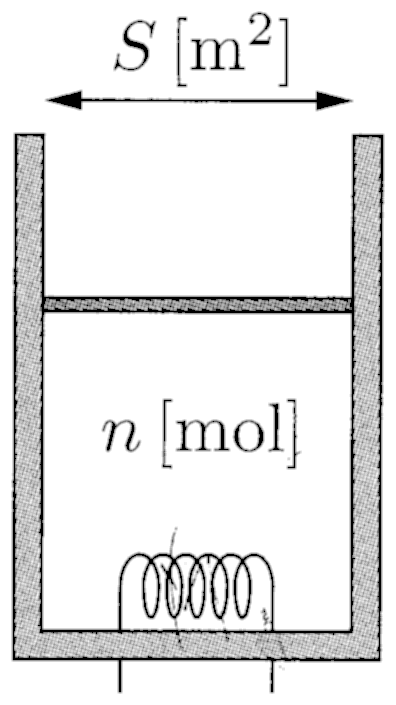
\includegraphics[keepaspectratio,width=24mm]{fig/ch16_p41_vcyl.png}
\end{zuright}
\begin{komon}
\ko{1} 初めの状態におけるシリンダー内の温度$T_0\U{K}$を求めよ．
\end{komon}
\hspace{1zw}この状態から内部の気体をヒーターで少しずつ熱したところ，ピストンはゆっくりと移動し，シリンダーの底からピストンまでの距離は$l_1\U{m}$となった．
\begin{komon}
\ko{2} 終状態における気体の温度$T_1\U{K}$を求めよ．
\ko{3} ヒーターによって気体に与えた熱量$Q\U{J}$を求めよ．
\end{komon}

\Mon{気体のした仕事}

\hspace{1zw}温度が$T_0\U{K}$の理想気体が$n\U{mol}$ある．この気体の温度を$T_0\U{K}$のまま一定に保ちつつ，体積を$V_1\U{m^3}$の状態$\mathrm{A}$から体積$V_2\U{m^3}$の状態$\mathrm{B}$へと膨張させる．気体定数を$R\U{J/mol\cdot K}$として以下の設問に答えよ．
\begin{komon}
\ko{1} この状態変化を$p$-$V$図で表せ．
\ko{2} この変化で気体が外界に対してした仕事$w$を求めよ．ただし，必要であれば積分公式$\displaystyle\int\frac{1}{x}dx=\log_e|x|+C$を用いよ．
\end{komon}

\Mon{定温変化}

\begin{zuright}{58mm}
\hspace{1zw}右図のように断面積$S\U{m^2}$のシリンダーの中に，ピストンで定積モル比熱が$C_V\U{J/mol\cdot K}$の理想気体を$n\U{mol}$だけ封入した．ピストンは軽くて自由に動くことができ，棒が取り付けられてある．
\zusep
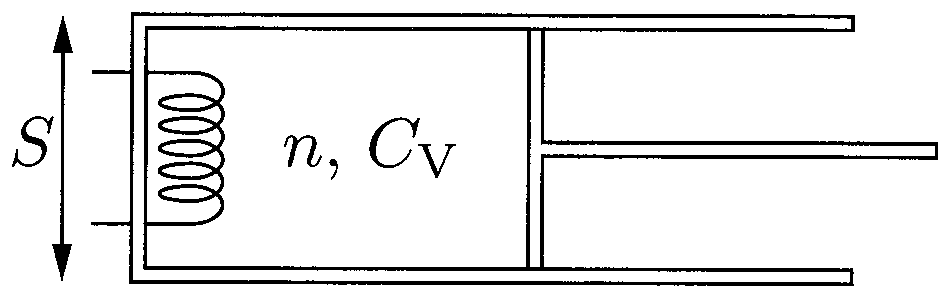
\includegraphics[keepaspectratio,width=58mm]{fig/ch17_p43_cyl.png}
\end{zuright}
\hspace{1zw}初め，シリンダーの底からピストンまでの距離は$l_0\U{m}$であり，また気体の温度は$T_0\U{K}$であった．シリンダー内にはヒーターが取り付けられており，気体に対して熱を与えることができる．シリンダーおよびピストンは断熱材でできており，ヒーターによって与えた熱が大気に拡散することはないものとする．気体定数を$R\U{J/mol\cdot K}$として以下の設問に答えよ．
\begin{komon}
\ko{1} 初めの状態におけるシリンダー内の気体の圧力$p_0\U{Pa}$を求めよ．
\end{komon}
\hspace{1zw}ここで，気体が温度$T_0\U{K}$を保つようにピストンを操作しながら内部の気体をヒーターでゆっくりと加熱したところ，ピストンはゆっくりと移動し，シリンダーの底からピストンまでの距離が$l_1\U{m}$となったところで加熱をやめた．
\begin{komon}
\ko{2} 終状態における気体の圧力$p_1\U{Pa}$を求めよ．
\ko{3} この変化において，気体が外界にした仕事$w\U{J}$を求めよ．
\ko{4} ヒーターによって加えた熱量$Q\U{J}$を求めよ．
\end{komon}

\Mon[\Sitei]{断熱変化}

\begin{zuright}{58mm}
\hspace{1zw}右図のように断面積$S\U{m^2}$のシリンダーの中に，ピストンで定積モル比熱が$C_V\U{J/mol\cdot K}$の理想気体を$n\U{mol}$だけ封入した．ピストンは軽くて自由に動くことができ，棒が取り付けられてある．
\zusep
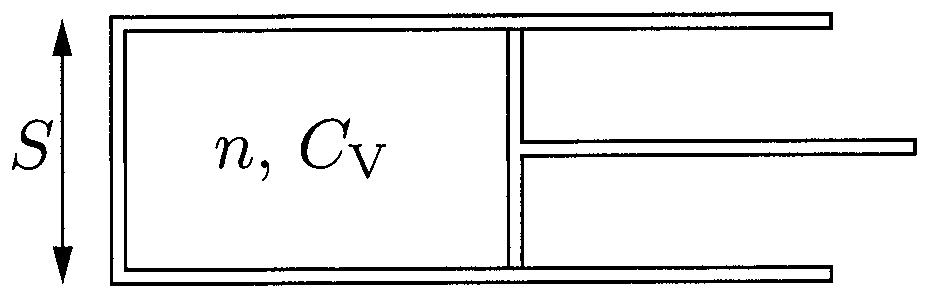
\includegraphics[keepaspectratio,width=58mm]{fig/ch17_p44_cyl.png}
\end{zuright}
\hspace{1zw}シリンダーおよびピストンは断熱材でできており，外界と熱のやり取りはない．棒を手で持って動かし，シリンダーの底からピストンまでの距離が$l_0\U{m}$となる位置に持ってきたところ気体の温度は$T_0\U{K}$となった．気体定数を$R\U{J/mol\cdot K}$として以下の設問に答えよ．
\begin{komon}
\ko{1} この状態におけるシリンダー内の圧力$p_0\U{Pa}$を求めよ．
\end{komon}
\hspace{1zw}ここでピストンを手でゆっくりと引き，シリンダーの底からピストンまでの距離が$l_1\U{m}$になるまで気体を膨張させた．
\begin{komon}
\ko{2} ポアソンの法則を用いて，終状態における気体の圧力$p_1\U{Pa}$および温度$T_1\U{K}$を求めよ．
% 誤植訂正（2026-09-02，旧 physics_ch17.tex から引き継ぎ）：原本は助詞「を」が欠けていた．
\ko{3} この状態変化を$p$-$V$図で表せ．
\ko{4} この変化において，気体が外界にした仕事$w\U{J}$を求めよ．
\end{komon}

\Mon{断熱自由膨張}

\begin{zuright}{56mm}
\hspace{1zw}右図のように，体積$V_\mathrm{A}\U{m^3}$, $V_\mathrm{B}\U{m^3}$の断熱容器A，Bをコックのついた細い管でつないである．はじめコックは閉じられており，Aだけに定積モル比熱$C_V\U{J/mol\cdot K}$の理想気体が圧力$p_0\U{Pa}$，温度$T_0\U{K}$となって入っている．コックを開いたところ気体はBへと拡散していき，十分時間が経つと全体が一様となった．このときA，B内の気体の圧力および温度を求めよ．ただし，気体定数を$R\U{J/mol\cdot K}$とする．
\zusep
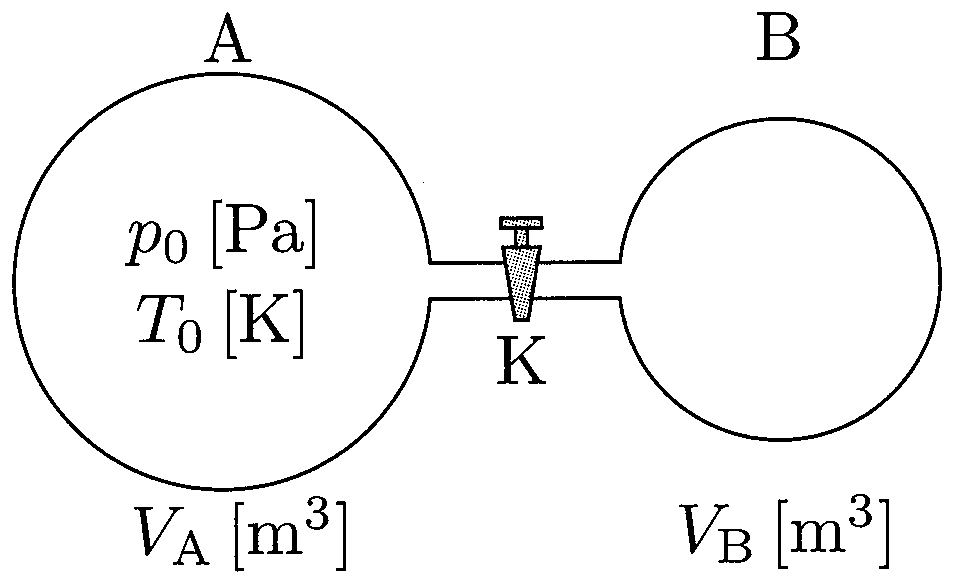
\includegraphics[keepaspectratio,width=56mm]{fig/ch17_p44_ab.png}
\end{zuright}

\Mon[\Sitei]{断熱膨張・断熱自由膨張}

\begin{zuright}{56mm}
\hspace{1zw}右図のようにバルブつきの隔壁で仕切られたシリンダーがある．隔壁の左側の体積は$V_0\U{m^3}$であり，ここに定積モル比熱$C_V\U{J/mol\cdot K}$の理想気体が圧力$p_0\U{Pa}$，温度$T_0\U{K}$となって封入されている．
\zusep
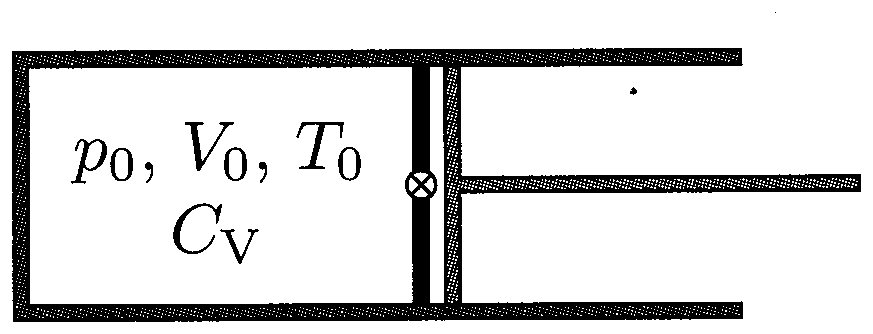
\includegraphics[keepaspectratio,width=56mm]{fig/ch17_p44_valve.png}
\end{zuright}
\hspace{1zw}隔壁の右側は取っ手付きのピストンが取り付けられている．初めバルブは閉じており，右側の空間には気体は封入されておらず，ピストンは隔壁に接触して体積が0になっている．シリンダー，ピストン，隔壁，バルブなどはすべて断熱材で出来ており，外界との熱のやり取りはない．

\hspace{1zw}この状態から以下の二つの方法によって左側に封入されている気体を右側に拡散させる．このとき，終状態における気体の圧力および温度をそれぞれ求めよ．気体定数を$R\U{J/mol\cdot K}$とする．
\begin{komon}
\ko{1} バルブを閉じたまま取っ手を引いて右側に体積$V_0\U{m^3}$の真空を作ったのち，バルブを全開にして気体を右側へ拡散させる．
\ko{2} バルブを全開にしてから取っ手をゆっくりと引き，右側の空間の体積を少しずつ増加させて体積$V_0\U{m^3}$にする．
\end{komon}

\Mon{状態変化に伴う各物理量の変化}

\hspace{1zw}ピストンのついた容器の中に一定量の気体を入れ，次の各変化を行う場合，\MARU{1}\MARU{2}\MARU{3}\MARU{4}に適するものを選べ．
\begin{komon}
\ko{1} 圧力を一定に保って圧縮させるとき
\ko{2} 体積を一定に保って減圧するとき
\ko{3} 温度を一定に保って加圧するとき
\ko{4} 外界との熱のやり取りを断ち切って圧縮するとき
\end{komon}
\hspace{1zw}各状態変化において，
\begin{list}{}{\setlength{\leftmargin}{2zw}\setlength{\itemsep}{0.4mm}\setlength{\topsep}{0.6mm}\setlength{\parsep}{0pt}}
\item[・] 外界が気体に与える熱量$Q$は，\fbox{\MARU{1}：正，\,0，\,負}となる．
\item[・] 外界が気体に対してする仕事$W$は，\fbox{\MARU{2}：正，\,0，\,負}となる．
\item[・] 気体の内部エネルギーの変化量$\Delta U$は，\fbox{\MARU{3}：正，\,0，\,負}となる．
\item[・] 気体の温度は，\fbox{\MARU{4}：上昇する，一定である，下降する}．
\end{list}

\Mon{サイクル（循環過程）}

\begin{zuright}{56mm}
\hspace{1zw}定積モル比熱が$C_V\U{J/mol\cdot K}$の理想気体をなめらかなピストンをもつシリンダーに封入し，右図の$p$-$V$図で示されるように$\mathrm{A}\rightarrow\mathrm{B}\rightarrow\mathrm{C}\rightarrow\mathrm{D}\rightarrow\mathrm{A}$の順でゆっくりと状態変化をさせた．状態$\mathrm{A}$の圧力は$p_0\U{Pa}$，体積は$V_0\U{m^3}$，温度は$T_0\U{K}$である．気体定数を$R\U{J/mol\cdot K}$として，以下の設問に答えよ．
\zusep
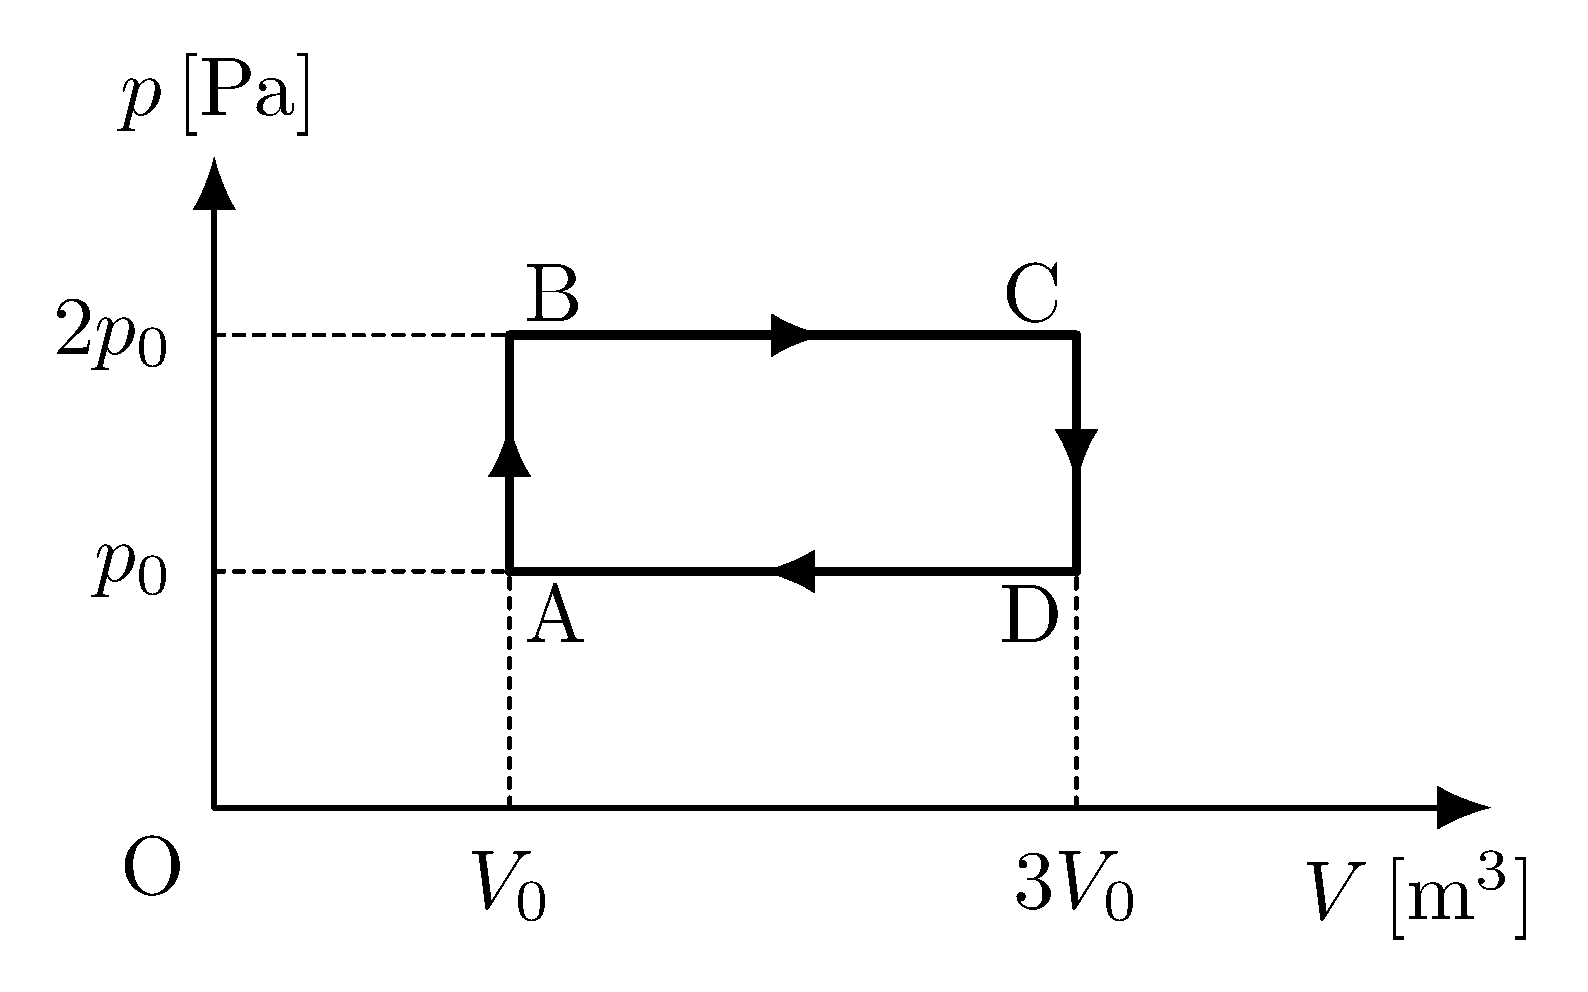
\includegraphics[keepaspectratio,width=56mm]{fig/n23_p31_pv.png}
\end{zuright}
\begin{komon}
\ko{1} 状態$\mathrm{B}$, $\mathrm{C}$, $\mathrm{D}$における気体の温度$T_{\mathrm{B}}\U{K}$, $T_{\mathrm{C}}\U{K}$, $T_{\mathrm{D}}\U{K}$を求めよ．
\ko{2} $T$-$V$図（横軸を$V$軸とする）を描け．ただしグラフには$\mathrm{A}$, $\mathrm{B}$, $\mathrm{C}$, $\mathrm{D}$点を明示し，変化の方向に矢印をつけること．
\ko{3} $\mathrm{A}$から$\mathrm{B}$, $\mathrm{C}$, $\mathrm{D}$を経て再び$\mathrm{A}$に戻ったとき，この間に気体が外界にした正味の仕事$W_{\mathrm{total}}\U{J}$（＝外界に対してなした仕事$-$外界からなされた仕事），および外界からもらった熱量$Q_{\mathrm{in}}\U{J}$（外界に対して捨てた熱量は含めない）を求めよ．
% 誤植訂正（2026-09-21）：原本の問題文は「外界からもらった熱量 $Q_1$[J]」だが，
%   解答では $Q_1\sim Q_4$ を各過程の吸熱量として使っており記号が衝突していた
%   （原本の指針・解答も「$Q_{\mathrm{in}}$」と書いている）．$Q_{\mathrm{in}}$ に統一した．
\ko{4} (3)で求めた値の比$\eta=\dfrac{W_{\mathrm{total}}}{Q_{\mathrm{in}}}$を熱効率という．この気体が上記のサイクルに沿って一巡したときの熱効率はいくらか．
\end{komon}

\Mon[\Sitei]{サイクル（循環過程）}

\begin{zuright}{52mm}
\hspace{1zw}定積モル比熱が$C_V\U{J/mol\cdot K}$の理想気体をなめらかなピストンをもつシリンダーに封入し，右図の$p$-$V$図で示されるように$\mathrm{A}\rightarrow\mathrm{B}\rightarrow\mathrm{C}\rightarrow\mathrm{A}$の順でゆっくりと状態変化させた（ただし，$\mathrm{B}\rightarrow\mathrm{C}$の過程は等温過程である）．状態$\mathrm{A}$の圧力を$p_0\U{Pa}$，体積を$V_0\U{m^3}$，温度を$T_0\U{K}$とし気体定数を$R\U{J/mol\cdot K}$として，以下の設問に答えよ．
% zuright の左が図より短いと差がまるごと空白になる（組版チェックリスト §3.10）ので，
%   (1) までを zuright の中に入れて図の高さに合わせた．
\begin{komon}
\ko{1} 状態変化$\mathrm{A}\rightarrow\mathrm{B}$, $\mathrm{B}\rightarrow\mathrm{C}$, $\mathrm{C}\rightarrow\mathrm{A}$について，気体が外界から熱を吸収した過程，および外界に対して熱を放出した過程はそれぞれどれか．
\end{komon}
\zusep
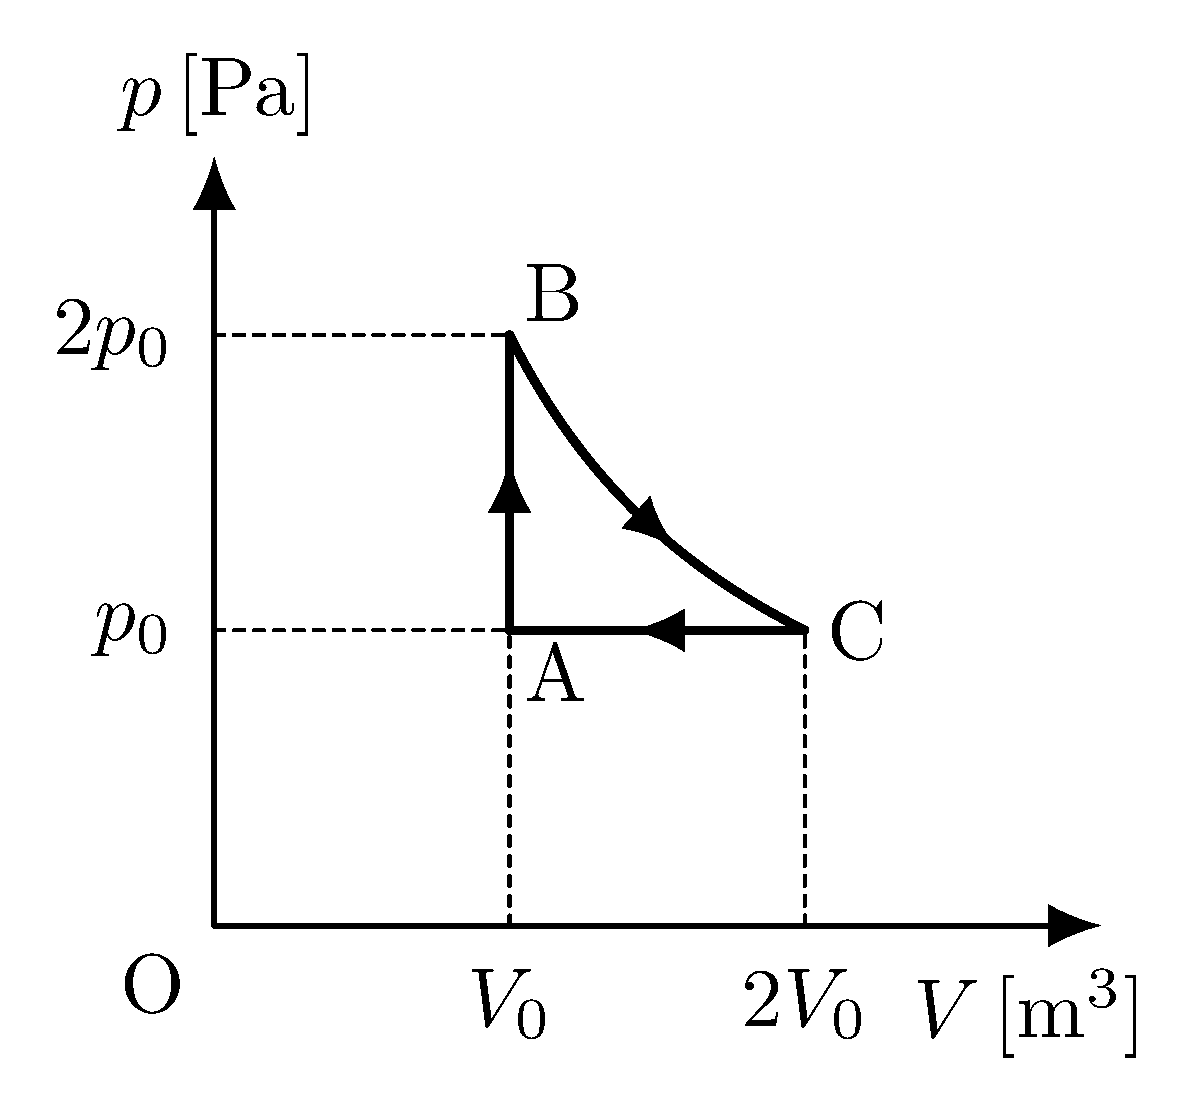
\includegraphics[keepaspectratio,width=52mm]{fig/n23_p32_pv.png}
\end{zuright}
\begin{komon}
\ko{2} $\mathrm{A}$から$\mathrm{B}$, $\mathrm{C}$を経て再び$\mathrm{A}$に戻ったとき，この間に気体が外界にした正味の仕事$w_{\mathrm{total}}\U{J}$（＝外界に対してなした仕事$-$外界からなされた仕事），および外界からもらった熱量$Q\U{J}$（外界に対して捨てた熱量は含めない）を求め，さらにこの気体が上記のサイクルに沿って一巡したときの熱効率$\eta=\dfrac{w_{\mathrm{total}}}{Q}$を求めよ．必要があれば積分公式$\displaystyle\int\frac{1}{x}dx=\log_e|x|+C$を用いよ．
\end{komon}

\filbreak
\Rank{C問題}

\Mon{気体の一般的な状態変化}

\begin{zuright}{62mm}
\hspace{1zw}図のように断面積$S\U{m^2}$のシリンダーに定積モル比熱が$C_V\U{J/mol\cdot K}$の理想気体を封入し，ピストンに図のように弾性定数が$k\U{N/m}$のバネを取り付けた．バネが自然長のとき，ちょうど大気圧$P_0\U{Pa}$とシリンダー内の気体の圧力とがつり合い，このときの気体の温度は$T_0\U{K}$，気柱の長さは$l_0\U{m}$であった．
\par
% 図が2枚縦積みで高いので，次の段落も zuright の中に入れて空白を埋めた（§3.10）
\hspace{1zw}シリンダー内のヒーターHから少しずつ気体を加熱していったところ，気体はゆっくりと膨張し，ピストンはゆっくりと距離$a\U{m}$だけ進んだ．シリンダー，容器などはすべて断熱材で出来ており，バネなどの熱容量は無視してよい．気体定数を$R\U{J/mol\cdot K}$として以下の設問に答えよ．
\zusep
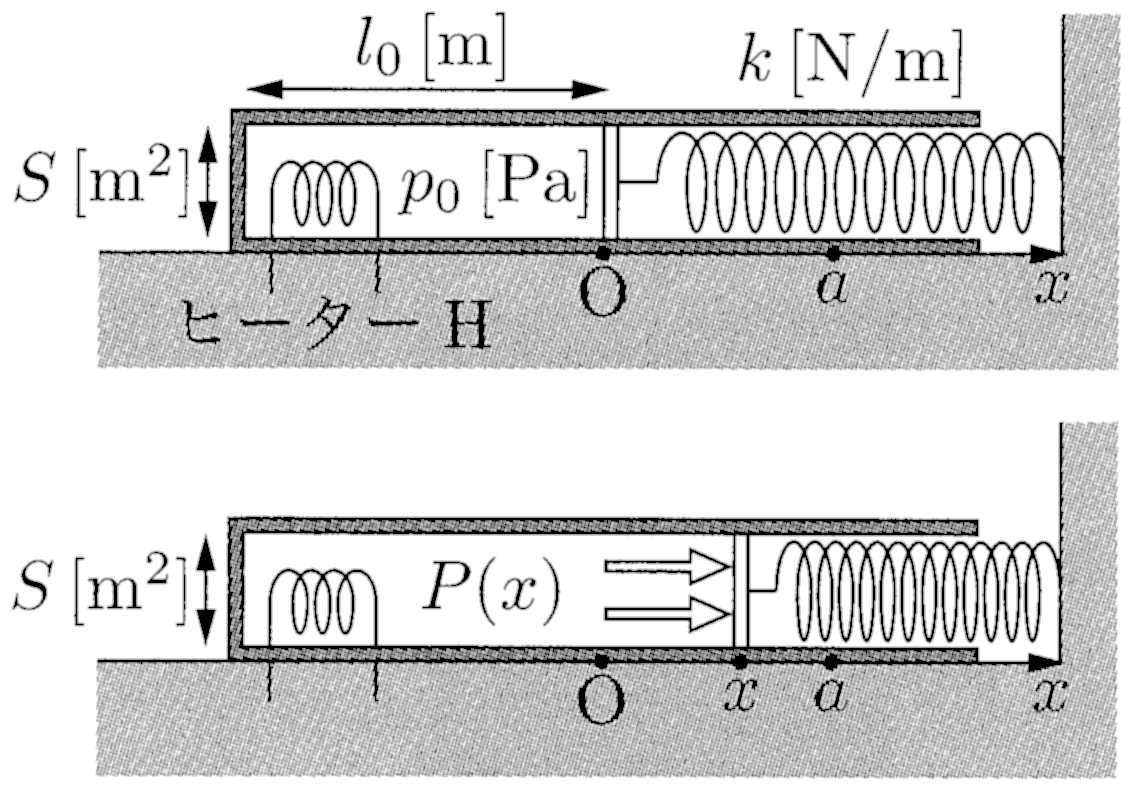
\includegraphics[keepaspectratio,width=62mm]{fig/ch17_p45_spring.png}
\end{zuright}
\begin{komon}
\ko{1} 終状態における気体の圧力$P_1\U{Pa}$および温度$T_1\U{K}$を求めよ．
\ko{2} この状態変化で気体がする仕事$w\U{J}$を求めよ．
\ko{3} この状態変化で気体に与えた熱量$Q\U{J}$を求めよ．
\end{komon}

\newpage

%%%%%%%%%%%%%%%%%%%%  解答  %%%%%%%%%%%%%%%%%%%%
\KaiTitle{第23回　気体の状態変化と熱機関}
\setlength{\columnseprule}{0.4pt}
\begin{multicols}{2}
\raggedcolumns

\Rank{A問題}
\MonN{22}{基本事項の確認}\par\nopagebreak
\begin{sisin}
(1)(2) 気体がした仕事は$\displaystyle\int P(V)dV$によって計算するが，特に定圧変化（$P(V)=p$（一定））の場合に限り，積分の中から$P(V)=p$を出して，$p\displaystyle\int dV=p\cdot\Delta V$と変形できる．

(3) 比熱比の定義式$\gamma=\dfrac{C_P}{C_V}$とマイヤーの関係式$C_P=C_V+R$を利用する．比熱比の分母・分子がどちらにくるかは，\underline{比熱比は}\hskip0pt\underline{必ず$1$}\hskip0pt\underline{より大}\hskip0pt\underline{きい}と覚えておけば間違いがない．
\end{sisin}
\KaiHead
\begin{komon}
\ko{1} $p=$一定のとき，気体の体積変化を$\Delta V$とすれば，気体が外界に対してする仕事$W$は，$W=p\Delta V$と表せるので，
% 誤植訂正（2026-09-02，旧 physics_ch16.tex から引き継ぎ）：原本は主語が「仕事」になっていた．
       \[\begin{aligned}
         W&=(1.0\times 10^5)\cdot(2.0\times 10^{-4})\\
          &=2.0\times 10\U{J}\Ans
       \end{aligned}\]
\ko{2} 熱力学第一法則$Q=\Delta U+w$より，$Q=4.2\times 10^3\U{J}$，$w=2.4\times 10^3\U{J}$であるから，
       \[\begin{aligned}
         \Delta U&=Q-w=4.2\times 10^3-2.4\times 10^3\\
                 &=1.8\times 10^3\U{J}\Ans
       \end{aligned}\]
\ko{3} マイヤーの関係式$C_P=C_V+R$を用いると，
       \[\gamma=\frac{C_P}{C_V}=1+\frac{R}{C_V}\]
       であるから，
       \[\text{単原子分子：}\gamma=1+\frac{R}{\frac{3}{2}R}=\frac{5}{3}\Ans\]
       \[\text{二原子分子：}\gamma=1+\frac{R}{\frac{5}{2}R}=\frac{7}{5}\Ans\]
\end{komon}

\Rank{B問題}
\MonN[\Sitei]{23}{気体がする仕事}\par\nopagebreak
\begin{sisin}
気体が外界に対してする仕事$w=$\hskip0pt$\displaystyle\int_{V_{\mathrm{initial}}}^{V_{\mathrm{final}}}P(V)dV$を計算する際，積分区間の下端には最初の状態の体積を，上端には最後の状態の体積を入れる．\underline{最後の状}\hskip0pt\underline{態の体積}\hskip0pt\underline{の方が小}\hskip0pt\underline{さいから}\hskip0pt\underline{といって}\hskip0pt\underline{下端に入}\hskip0pt\underline{れてはな}\hskip0pt\underline{らない！}

$w=\displaystyle\int_{V_{\mathrm{initial}}}^{V_{\mathrm{final}}}P(V)dV$から分かるように，$V_{\mathrm{final}}>V_{\mathrm{initial}}$の場合には気体が外部にする仕事$w$は$p$-$V$図の曲線と$V$軸とで囲まれる部分の面積を表す．

一方，$V_{\mathrm{final}}<V_{\mathrm{initial}}$の際には$p$-$V$図の曲線と$V$軸とで囲まれる部分の面積は$\displaystyle\int_{V_{\mathrm{final}}}^{V_{\mathrm{initial}}}P(V)dV$と表される．これは{\gtfamily 気体が外界からされた仕事}を表す．気体が外部にする仕事は，これにマイナスをつけた値である．
\end{sisin}
\KaiHead
\begin{komon}
\ko{1} 次の長方形の面積が求める値である．
       \begin{center}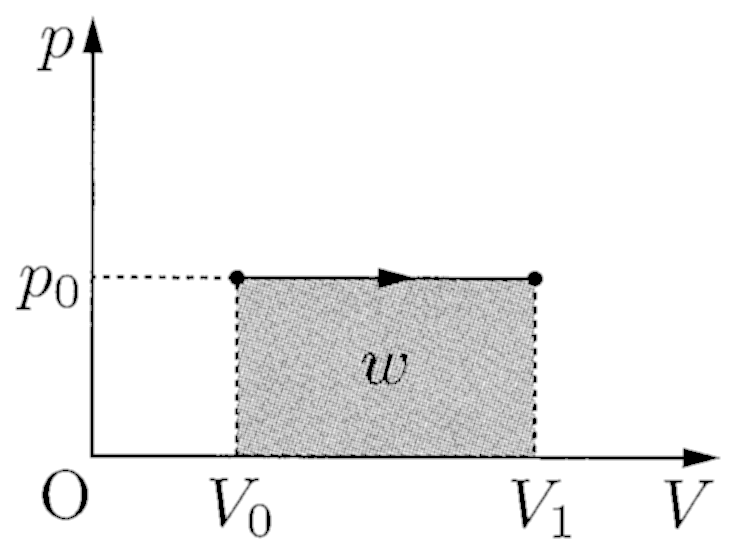
\includegraphics[keepaspectratio,width=46mm]{fig/ch16_a18_1.png}\end{center}
       \[w=p_0(V_1-V_0)\U{J}\Ans\]
\ko{2} 次の台形の面積が求める値である．
       \begin{center}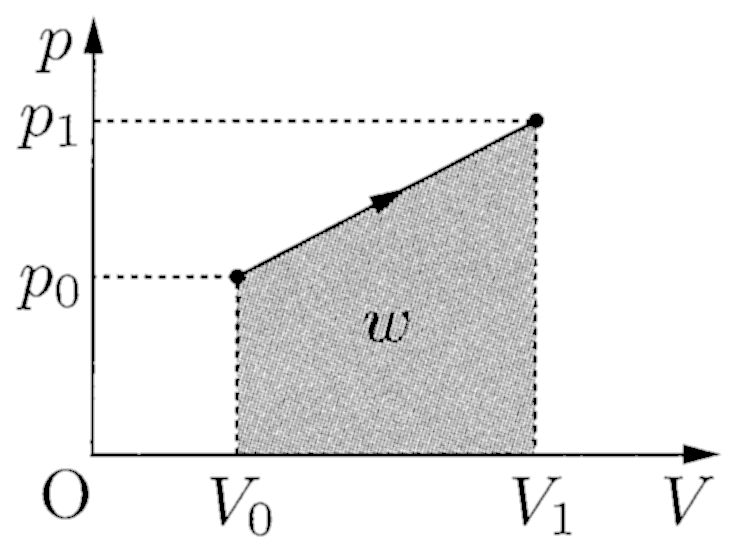
\includegraphics[keepaspectratio,width=46mm]{fig/ch16_a18_2.png}\end{center}
       \[w=\frac{1}{2}(p_0+p_1)(V_1-V_0)\U{J}\Ans\]
\ko{3} 気体の体積変化がないので，
       \[w=0\U{J}\Ans\]
\ko{4} 次の網点部の面積が求める値である．
       \begin{center}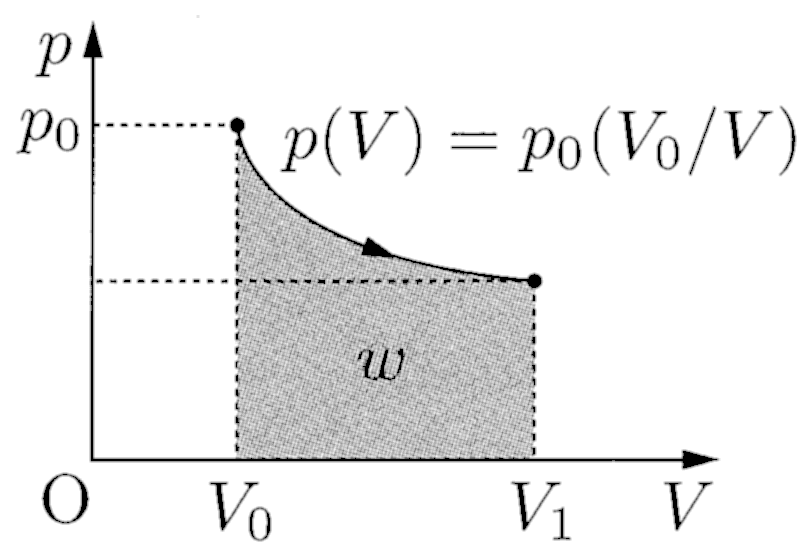
\includegraphics[keepaspectratio,width=48mm]{fig/ch16_a18_4.png}\end{center}
       \[\begin{aligned}
         w&=\int_{V_0}^{V_1}\frac{p_0V_0}{V}dV=p_0V_0\Bigl[\log_e|V|\Bigr]_{V_0}^{V_1}\\
          &=p_0V_0\log_e\frac{V_1}{V_0}\U{J}\Ans
       \end{aligned}\]
\ko{5} 気体が外部からされる仕事を$W$とすると，
       \[W=p_0(V_0-V_1)\U{J}\]
       \begin{center}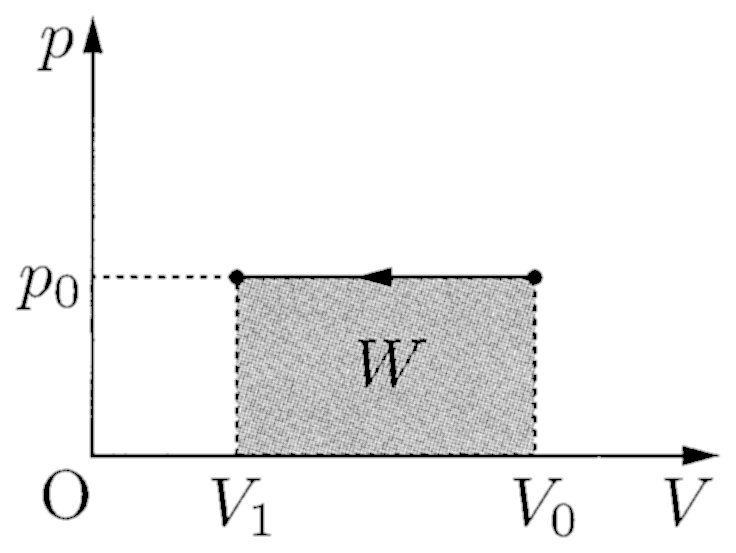
\includegraphics[keepaspectratio,width=46mm]{fig/ch16_a18_5.png}\end{center}
       求めるのは気体が外部にする仕事であるから，
       \[w=-W=-p_0(V_0-V_1)\U{J}\Ans\]
\ko{6} この場合，下の網点部の面積が$W$に等しい．
       \begin{center}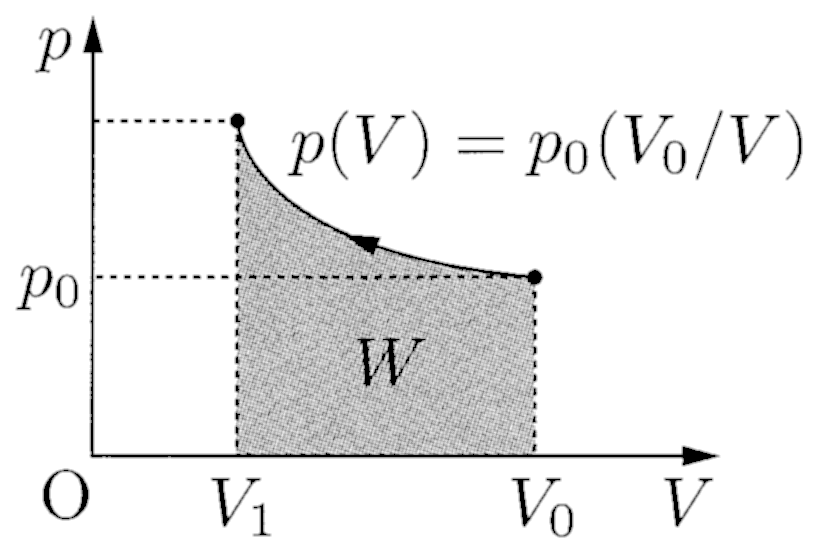
\includegraphics[keepaspectratio,width=48mm]{fig/ch16_a18_6.png}\end{center}
       \[\begin{aligned}
         W&=\int_{V_1}^{V_0}\frac{p_0V_0}{V}dV=p_0V_0\Bigl[\log_e|V|\Bigr]_{V_1}^{V_0}\\
          &=p_0V_0\log_e\frac{V_0}{V_1}\U{J}
       \end{aligned}\]
       求めるのは気体が外部にする仕事であるから，
       \[w=-W=-p_0V_0\log_e\frac{V_0}{V_1}\U{J}\Ans\]
\end{komon}
\begin{bekkai}
各問について$w=\displaystyle\int_{\mathrm{start}}^{\mathrm{end}}P(V)dV$を考えると，
\begin{komon}
\ko{1} $w=\displaystyle\int_{V_0}^{V_1}p_0dV=p_0(V_1-V_0)\U{J}$\Ans
\ko{2} 与えられたグラフより
       \[p(V)=p_0+\frac{p_1-p_0}{V_1-V_0}(V-V_0)\]
       であるから，
       \[\begin{aligned}
         w&=\int_{V_0}^{V_1}\left\{p_0+\frac{p_1-p_0}{V_1-V_0}(V-V_0)\right\}dV\\
          &=\frac{p_0+p_1}{2}(V_1-V_0)\U{J}\Ans
       \end{aligned}\]
% 誤植訂正（2026-09-02，旧 physics_ch16.tex から引き継ぎ）：原本は $\frac{p_1+p_2}{2}$．
%   本問に $p_2$ は登場しない．
\ko{3} $w=\displaystyle\int_{V_0}^{V_0}P(V)dV=0\U{J}$\Ans
\ko{4} $w=\displaystyle\int_{V_0}^{V_1}\frac{p_0V_0}{V}dV=p_0V_0\Bigl[\log_e|V|\Bigr]_{V_0}^{V_1}$\par
       \hspace*{1zw}$=p_0V_0\log_e\dfrac{V_1}{V_0}\U{J}$\Ans
\ko{5} $w=\displaystyle\int_{V_0}^{V_1}p_0dV=-p_0(V_0-V_1)\U{J}$\Ans
\ko{6} $w=\displaystyle\int_{V_0}^{V_1}\frac{p_0V_0}{V}dV=p_0V_0\Bigl[\log_e|V|\Bigr]_{V_0}^{V_1}$\par
       \hspace*{1zw}$=-p_0V_0\log_e\dfrac{V_0}{V_1}\U{J}$\Ans
\end{komon}
\end{bekkai}
\begin{chuu}
(5), (6)の答えにおいてマイナスを前に出したのは，$V_0>V_1$であるため．このような形にした方が式の正負がはっきり分かる．
\end{chuu}

\MonN[\Sitei]{24}{鉛直シリンダー}\par\nopagebreak
\begin{sisin}
質量$M\U{kg}$のピストンが気体の上に乗っているので，気体の圧力は大気圧$p_0\U{Pa}$と等しくはならない．このような場合には，\underline{ピストン}\hskip0pt\underline{に対して}\hskip0pt\underline{かかる力}\hskip0pt\underline{のつり合}\hskip0pt\underline{いの式を}\hskip0pt\underline{立てて}気体の圧力を求める．

(2)ではピストンがゆっくり動くことから，各瞬間においてピストンに働く力はつりあっていると見なせる．このような変化を準静的変化という．
\end{sisin}
\KaiHead
\begin{komon}
\ko{1} 初状態におけるシリンダー内の圧力を$p\U{Pa}$とする．力の作用図は次図の通りであり，ピストンは静止しているので作用する力がつり合っている．
       \begin{center}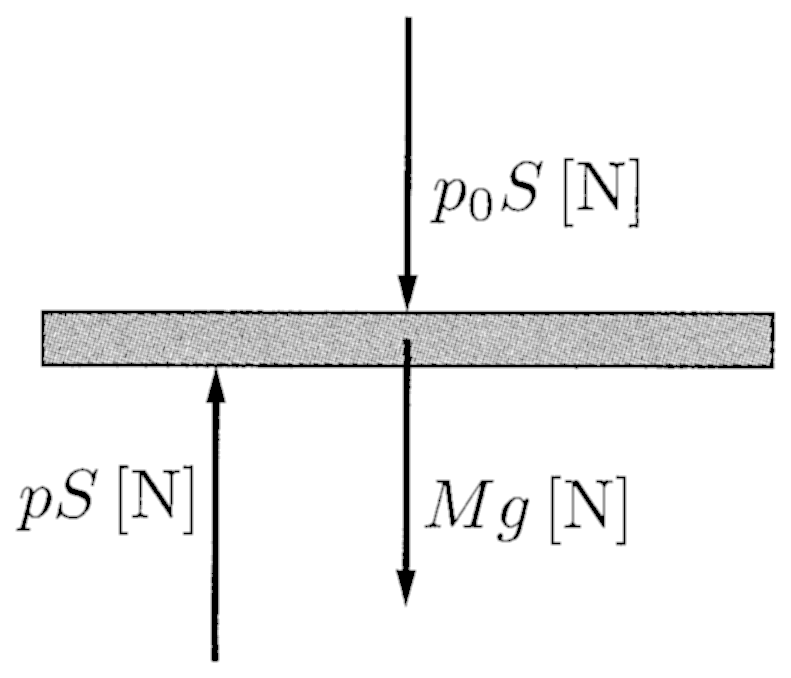
\includegraphics[keepaspectratio,width=44mm]{fig/ch16_a22_f1.png}\end{center}
       この状態の力のつり合いの式は，
       \[pS=p_0S+Mg\]
       ゆえに，
       \[p=p_0+\frac{Mg}{S}\U{Pa}\]
       また，このときの理想気体の状態方程式は，
       \[p(Sl_0)=nRT_0\]
       であるから，これを解いて気体の温度は，
       \[T_0=\frac{(p_0S+Mg)l_0}{nR}\U{K}\Ans\]
\ko{2} ゆっくりと加熱しているからピストンはゆっくりと動いている．よって，このピストンは力のつり合いを保ちつつ動いていると考えられる．変化途中，ピストンに対して作用する力は，(1)と同じく，大気圧による力，気体の圧力による力，重力の三つである．
       \begin{center}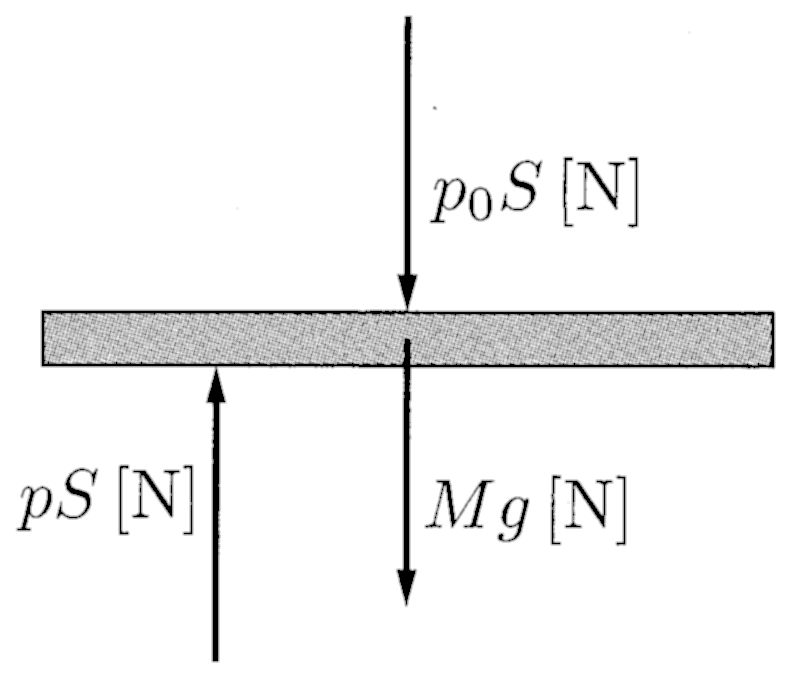
\includegraphics[keepaspectratio,width=44mm]{fig/ch16_a22_f2.png}\end{center}
       よって，変化している最中，ピストンの力のつり合いの式はずっと
       \[pS=p_0S+Mg\]
       のまま変わらないため，内部の気体の圧力は
       \[p=p_0+\frac{Mg}{S}\U{Pa}\]
       のまま変わらない．すなわち，この気体は定圧変化を行う．\par
       \hspace*{1zw}よって，終状態でも気体の圧力は
       \[p=p_0+\frac{Mg}{S}\U{Pa}\]
       であり，終状態での状態方程式
       \[p(Sl_1)=nRT_1\]
       を解いて，
       \[T_1=\frac{(p_0S+Mg)l_1}{nR}\U{K}\Ans\]
\ko{3} 以上より，この気体の状態変化を$p$-$V$図で表すと次図の通り．
       \begin{center}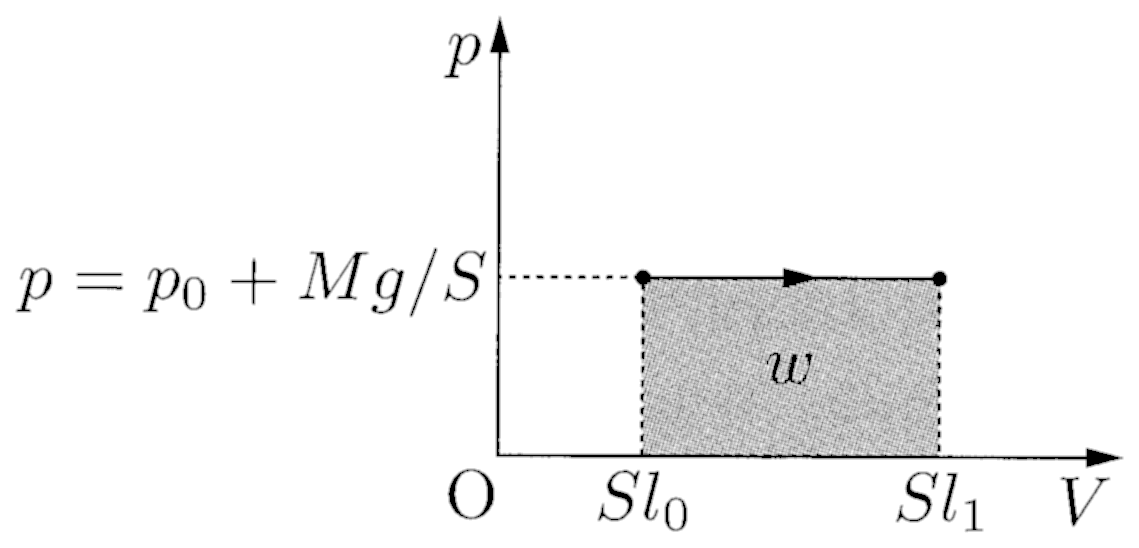
\includegraphics[keepaspectratio,width=66mm]{fig/ch16_a22_pv.png}\end{center}
       よって，この状態変化で気体が外界に対してした仕事$w$は
       \[\begin{aligned}
         w&=\int_{Sl_0}^{Sl_1}pdV=\int_{Sl_0}^{Sl_1}\left(p_0+\frac{Mg}{S}\right)dV\\
          &=(p_0S+Mg)(l_1-l_0)\U{J}\ \cdots\mbox{☆}
       \end{aligned}\]
       また，この変化における気体の内部エネルギーの変化は，
       \[\begin{aligned}
         \Delta U&=nC_V(T_1-T_0)\\
                 &=\frac{C_V(p_0S+Mg)(l_1-l_0)}{R}\U{J}
       \end{aligned}\]
       ここで熱力学第一法則より，$\Delta U$, $Q$, $w$の間には
       \[Q=\Delta U+w\]
       の関係が成り立つので，
       \[Q=(p_0S+Mg)(l_1-l_0)\left(1+\frac{C_V}{R}\right)\U{J}\Ans\]
\end{komon}
\begin{bekkai}
この変化は定圧変化であるから，その吸熱量は
\[Q=nC_P(T_1-T_0)\]
である．マイヤーの関係式より$C_P=C_V+R$であるから，
\[Q=n(C_V+R)(T_1-T_0)\]
としても同じ答えを得る．
\end{bekkai}
\begin{bsHosoku}{参考}
☆式にて気体の圧力を積分して$w$を得たが，結果としてその$w$は何に利用されたのかを考えると，
\[w=p_0S(l_1-l_0)+Mg(l_1-l_0)\U{J}\]
と変形すれば，第一項目は大気圧に逆らった仕事，そして第二項目はピストンを持ち上げた位置エネルギー増分であることが分かる．すなわち，$w$は積分を実行しなくても求めることもできる．

$w$が何に利用されるのか直観的に明らかな場合も多いが，より厳密には気体の圧力$p$を与えている式を見れば分かる．$p=p_0+\dfrac{Mg}{S}\U{Pa}$であるのだから，気体が膨張するということは，$p_0$および$\dfrac{Mg}{S}$を押す，ということを意味する．よって，$w$は大気圧に逆らう仕事とピストンを持ち上げる仕事の二つに利用される．本問程度の問題の場合はわざわざこのようなことを考える必要はないが，複雑な問題の場合（バネを含む場合など）はこのことを考えて$w$を求めた方が容易なこともある．
\end{bsHosoku}

\MonN{25}{気体のした仕事}\par\nopagebreak
\begin{sisin}
要するに$w=\displaystyle\int_{V_{\mathrm{initial}}}^{V_{\mathrm{final}}}P(V)dV$を計算すればよいのだから，変化途中の，体積が$V\U{m^3}$になったときの圧力$P(V)$を求め，これを積分すればよい．
\end{sisin}
\KaiHead
\begin{komon}
\ko{1} 膨張前・膨張後の圧力をそれぞれ$P_1$, $P_2\U{Pa}$として気体の状態方程式を立てると，
       \[P_1V_1=nRT_0,\ P_2V_2=nRT_0\]
       である．また，変化途中の体積が$V\U{m^3}$になったときの圧力$P(V)$は，その時の状態方程式
       \[P(V)V=nRT_0\]
       より，
       \[P(V)=\frac{nRT_0}{V}\U{Pa}\]
       である．この式の分子は定数であるから，気体の圧力は体積に反比例して変化する．すなわち，$p$-$V$図は双曲線となるので，状態変化の$p$-$V$図は次図．
       \begin{center}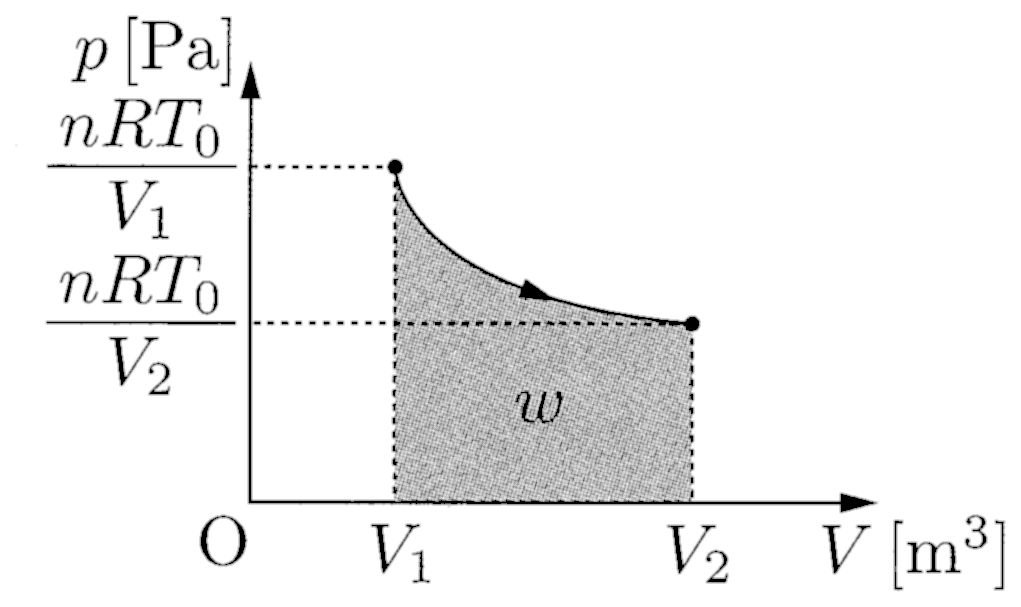
\includegraphics[keepaspectratio,width=60mm]{fig/ch16_a21_pv.png}\end{center}
       \hspace*{\fill}\Ans
\ko{2} 気体は膨張しているので，上の$p$-$V$図の網点部が気体が外部にした仕事$w$を表す．よって，
       \[\begin{aligned}
         w&=\int_{V_1}^{V_2}\frac{nRT_0}{V}dV=nRT_0\Bigl[\log_e|V|\Bigr]_{V_1}^{V_2}\\
          &=nRT_0\log_e\frac{V_2}{V_1}\U{J}\Ans
       \end{aligned}\]
       これは 23.2 のまとめ枠の式そのものである．
\end{komon}

\MonN{26}{定温変化}\par\nopagebreak
\begin{sisin}
本問のように，変化途中で気体の圧力が変化する場合には$w=P\cdot\Delta V$としてはいけない．体積が$V\U{m^3}$のときの圧力$P(V)\U{Pa}$を求め，これを積分することで求める．
\end{sisin}
\KaiHead
\begin{komon}
\ko{1} 最初の状態について状態方程式を立てると，
       \[p_0\cdot Sl_0=nRT_0\]
       であるから，
       \[p_0=\frac{nRT_0}{Sl_0}\U{Pa}\Ans\]
\ko{2} 終状態における状態方程式は，
       \[p_1\cdot Sl_1=nRT_0\]
       であるから，
       \[p_1=\frac{nRT_0}{Sl_1}\U{Pa}\Ans\]
\ko{3} 気体の体積が$V\U{m^3}$のときの気体の圧力を$p(V)\U{Pa}$とし，このときの気体の状態方程式を立てると，
       \[p(V)\cdot V=nRT_0\]
       これより，
       \[p(V)=\frac{nRT_0}{V}\]
       よって，体積が$V=Sl_0\rightarrow Sl_1\U{m^3}$に変化するまでに気体が外部にした仕事$w$は，$nRT_0$が定数であることに注意して
       \[\begin{aligned}
         w&=\int_{Sl_0}^{Sl_1}p(V)dV=\int_{Sl_0}^{Sl_1}\frac{nRT_0}{V}dV\\
          &=nRT_0\int_{Sl_0}^{Sl_1}\frac{1}{V}dV\\
          &=nRT_0\Bigl[\log_e|V|\Bigr]_{Sl_0}^{Sl_1}\\
          &=nRT_0\log_e\frac{l_1}{l_0}\U{J}\Ans
       \end{aligned}\]
\ko{4} この状態変化にて気体の温度は$T_0$一定であるから，気体の内部エネルギー変化$\Delta U\U{J}$は
       \[\Delta U=nC_V\Delta T=0\]
       である．熱力学第一法則より$Q$, $\Delta U$, $w$の間には，
       \[Q=\Delta U+w\]
       の関係が成り立つ．以上より気体に加えた熱量は
       \[Q=nRT_0\log_e\frac{l_1}{l_0}\U{J}\Ans\]
\end{komon}

\MonN[\Sitei]{27}{断熱変化}\par\nopagebreak
\begin{sisin}
ピストンはゆっくりと移動するので，この状態変化は準静的過程である．理想気体の均一系準静的断熱変化では，ポアソンの式
\[PV^\gamma=（一定）,\;TV^{\gamma-1}=（一定）\]
が成立する．どちらの式を利用した方がよいかは問題文に与えられている文字で考えよ．本問では$p$, $T$の両方が問われているのでどちらを利用してもよい．前者の$pV^\gamma=（一定）$で考えた場合を示す．

断熱曲線の勾配は等温曲線よりも急になる．

\underline{断熱変化の}\hskip0pt\underline{場合に限}\hskip0pt\underline{り，$w$を}\hskip0pt\underline{熱力学第}\hskip0pt\underline{一法則か}\hskip0pt\underline{ら求める}\hskip0pt\underline{ことがで}\hskip0pt\underline{きる}．断熱変化の場合は$Q=0$であるから，$\Delta U$から$w$を求めることができるのである．もちろん$w=\displaystyle\int_{V_{\mathrm{initial}}}^{V_{\mathrm{final}}}P(V)dV$から求めることも可能である．
\end{sisin}
\KaiHead
気体の比熱比$\gamma$は，マイヤーの関係式を用いて，
\[\gamma=\frac{C_P}{C_V}=\frac{C_V+R}{C_V}=1+\frac{R}{C_V}\]
で与えられる．
\begin{komon}
\ko{1} 初めの状態について状態方程式を立てると，
       \[p_0Sl_0=nRT_0\]
       これを解いて，
       \[p_0=\frac{nRT_0}{Sl_0}\U{Pa}\Ans\]
\ko{2} 気体は外界と熱のやり取りをしておらず，断熱変化であるので，初状態と終状態に対してポアソンの式より，
       \[p_0(Sl_0)^\gamma=p_1(Sl_1)^\gamma\]
       が成り立つ．これを解いて，
       \[p_1=\frac{nRT_0}{Sl_0}\left(\frac{l_0}{l_1}\right)^{1+\frac{R}{C_V}}\U{Pa}\Ans\]
       また，終状態の状態方程式は，
       \[p_1Sl_1=nRT_1\]
       であるから，これを解いて
       \[T_1=T_0\left(\frac{l_0}{l_1}\right)^{\frac{R}{C_V}}\U{K}\Ans\]
       \begin{bekkai}
       もう一つのポアソンの式$TV^{\gamma-1}=$一定を利用してもよい．この場合は，$\gamma-1=\dfrac{R}{C_V}$より
       \[T_0(Sl_0)^{\gamma-1}=T_1(Sl_1)^{\gamma-1}\]
       より，$T_1=T_0\left(\dfrac{l_0}{l_1}\right)^{\frac{R}{C_V}}\U{K}$を導くことができる．また，この$T_1$を元に終状態の状態方程式$p_1Sl_1=nRT_1$を立てて圧力$p_1$を求めることが可能である．

       ポアソンの式は多少面倒な式であるから，まず$pV^\gamma=$一定もしくは$TV^{\gamma-1}=$一定を用いて変化後の$p$, $T$のいずれか一方を求め，もう片方については状態方程式から求めればよい．両方をポアソンの式から求めるのは面倒なだけである．
       \end{bekkai}
\ko{3} 気体の体積が$V\U{m^3}$のときの気体の圧力を$p(V)\U{Pa}$とし，初状態とこの状態との間にポアソンの式より，
       \[p(V)V^\gamma=p_0(Sl_0)^\gamma\quad(=\text{一定})\]
       が成り立つ．よって，
       \[p(V)=p_0(Sl_0)^\gamma\frac{1}{V^\gamma}\]
       である．ここで$\gamma>1$に注意すると，これは右下がりの曲線を表すので，状態変化の$p$-$V$図は次図の通り．
       \begin{center}
       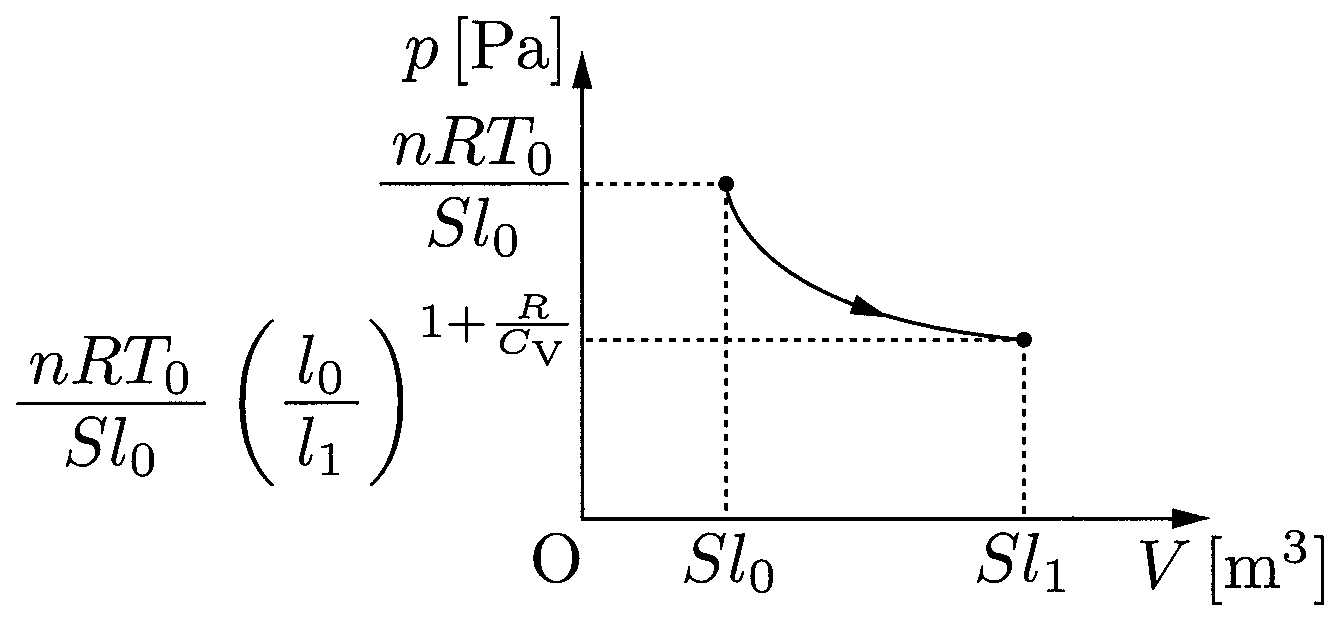
\includegraphics[keepaspectratio,width=64mm]{fig/ch17_a27_pv.png}
       \end{center}
       \hspace*{\fill}\Ans
\ko{4} この変化は断熱変化であるから，外部が気体に与える熱量$Q$は，
       \[Q=0\]
       また，この状態変化の内部エネルギーの増加量$\Delta U$は，
       \[\begin{aligned}
         \Delta U&=nC_V(T_1-T_0)\\
                 &=nC_VT_0\left\{\left(\frac{l_0}{l_1}\right)^{\frac{R}{C_V}}-1\right\}\U{J}
       \end{aligned}\]
       気体が外界に対してした仕事$w$は，熱力学第一法則を用いると，
       \[Q=\Delta U+w\]
       の関係があるので，
       \[\begin{aligned}
         w&=-\Delta U\\
          &=nC_VT_0\left\{1-\left(\frac{l_0}{l_1}\right)^{\frac{R}{C_V}}\right\}\U{J}\Ans
       \end{aligned}\]
       \begin{bekkai}
       指針でも述べたように，まともに
       \[w=\int_{V_{\mathrm{initial}}}^{V_{\mathrm{final}}}P(V)dV\]
       を計算しても同一の答えが求められる．気体の体積が$V\U{m^3}$のときの気体の圧力$p(V)\U{Pa}$は，
       \[p(V)=p_0(Sl_0)^\gamma\frac{1}{V^\gamma}\]
       であるから，
       \[\begin{aligned}
         w&=\int_{Sl_0}^{Sl_1}p(V)dV\\
          &=p_0(Sl_0)^\gamma\int_{Sl_0}^{Sl_1}\frac{1}{V^\gamma}dV\\
          &=p_0(Sl_0)^\gamma\left[\frac{1}{-\gamma+1}V^{-\gamma+1}\right]_{Sl_0}^{Sl_1}\\
          &=p_0(Sl_0)^\gamma\left[-\frac{C_V}{R}\cdot\frac{1}{V^{\gamma-1}}\right]_{Sl_0}^{Sl_1}\\
          &=-\frac{C_V}{R}p_0(Sl_0)^{\gamma-1}(Sl_0)\\
          &\qquad\times\left\{\frac{1}{(Sl_1)^{\gamma-1}}-\frac{1}{(Sl_0)^{\gamma-1}}\right\}\\
          &=-\frac{C_V}{R}p_0(Sl_0)\left\{\left(\frac{l_0}{l_1}\right)^{\gamma-1}-1\right\}\\
          &=\frac{C_V}{R}\frac{nRT_0}{Sl_0}Sl_0\left\{1-\left(\frac{l_0}{l_1}\right)^{\frac{R}{C_V}}\right\}\\
          &=nC_VT_0\left\{1-\left(\frac{l_0}{l_1}\right)^{\frac{R}{C_V}}\right\}\U{J}
       \end{aligned}\]
       となり，全く同じ答えが導ける．しかし，この計算はなかなかに厄介である．断熱変化に限っては熱力学第一法則から$w$を求めることを覚えておくとよい．
       \end{bekkai}
\end{komon}

\MonN{28}{断熱自由膨張}\par\nopagebreak
\begin{sisin}
本問のような断熱自由膨張では，\underline{容器$\mathrm{A+B}$}\hskip0pt\underline{全体を一}\hskip0pt\underline{つの系と}\hskip0pt\underline{みなして}\hskip0pt\underline{熱力学第}\hskip0pt\underline{一法則を}\hskip0pt\underline{立てる}のがポイント．$\mathrm{A+B}$の全体積は$V_\mathrm{A}+V_\mathrm{B}\U{m^3}$のまま不変であるから，$\mathrm{A+B}$は容器外と仕事のやり取りをしない．また，断熱容器を使っているから熱のやり取りもない．以上に着目して熱力学第一法則を立てる．
\end{sisin}
\KaiHead
変化後の$\mathrm{A}$, $\mathrm{B}$内の気体の圧力を$p\U{Pa}$, 温度を$T\U{K}$とする．この変化において，$\mathrm{A+B}$を一つの系とみなすと，これは体積が不変であるから外界と仕事のやり取りをせず，また断熱容器を利用しているので外界と熱のやり取りもしない．よって，内部エネルギーの変化量を$\Delta U$とすると，熱力学第一法則より，
\[\Delta U=0-0=0\]
と立式できる．$\Delta U$は絶対温度に比例し，
\[\Delta U=nC_V\Delta T=0\]
と表せるので，これより$\Delta T=0$, すなわち気体の温度は変化しない．
\[T=T_0\U{K}\Ans\]
また状態変化前の$\mathrm{A}$内の気体のモル数を$n$とすると，状態方程式は，
\[p_0V_\mathrm{A}=nRT_0\]
また状態変化後は$\mathrm{A+B}$に一様に気体が広がっているので$\mathrm{A+B}$全体に対して状態方程式を立てることができ，
\[p(V_\mathrm{A}+V_\mathrm{B})=nRT_0\]
となる．以上2式を組み合わせて，
\[p=\frac{V_\mathrm{A}}{V_\mathrm{A}+V_\mathrm{B}}p_0\U{Pa}\Ans\]

\MonN[\Sitei]{29}{断熱膨張・断熱自由膨張}\par\nopagebreak
\begin{sisin}
(1)も(2)もいずれも断熱変化であり，最終的には全体積$2V_0\U{m^3}$の空間に気体が広がることになるが，(1)の方法と(2)の方法は全く異なる．(1)は前問と全く同じで，真空中への拡散である．一方，(2)は，バルブを全開にしてからゆっくりと引いているのだから，バルブはないのと同じことである．よって，これは準静的な断熱膨張で，ポアソンの式を利用して考えればよい．
\end{sisin}
\KaiHead
気体のモル数を$n\U{mol}$とすると，最初の状態の状態方程式は
\[p_0V_0=nRT_0\]
である．
\begin{komon}
\ko{1} この方法では，次図のようにいったん右側に体積$V_0\U{m^3}$の真空を作り，左側から右側へ気体を拡散させていくので断熱自由膨張だとみなせる．
       \begin{center}
       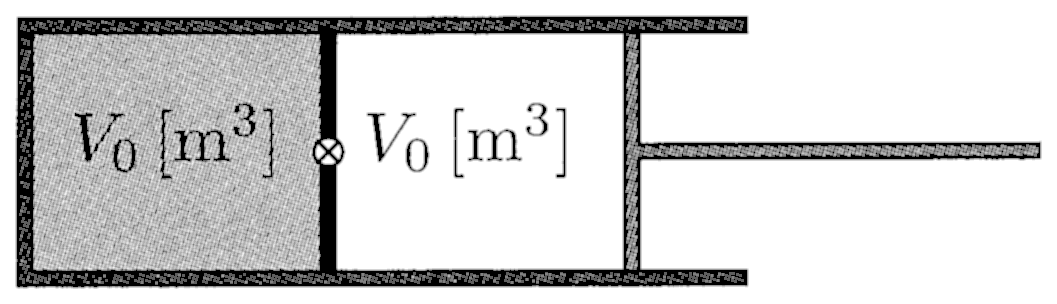
\includegraphics[keepaspectratio,width=62mm]{fig/ch17_a29_1.png}
       \end{center}
       よって，左側の空間と右側の空間を一つの系だとみなすと，この系は外界との仕事のやり取り，熱のやり取りがない．内部エネルギーの変化量を$\Delta U\U{J}$とすると，熱力学第一法則より$\Delta U=0-0=0$となる．内部エネルギーは絶対温度に比例するので，全体に拡がる前後で温度変化はなく，変化後の気体の温度を$T_1\U{K}$とおくと，
       \[T_1=T_0\U{K}\Ans\]
       また，このときの気体の圧力を$p_1\U{Pa}$とする．最終的には容器全体に気体が一様に拡がっているので，全体に対して状態方程式を立てることができ，
       \[p_1\cdot 2V_0=nRT_0\]
       \begin{center}
       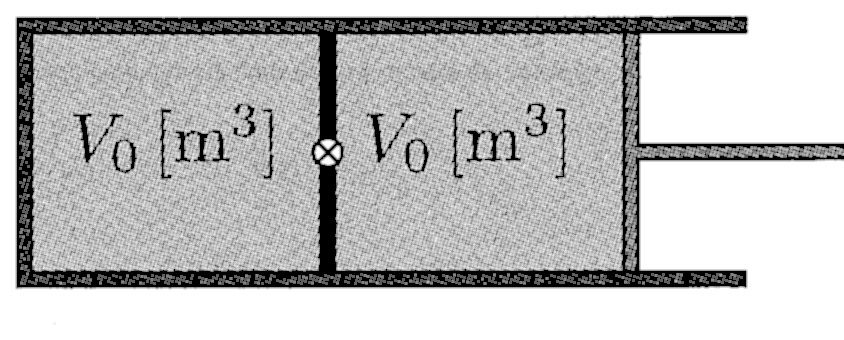
\includegraphics[keepaspectratio,width=54mm]{fig/ch17_a29_2.png}
       \end{center}
       これと最初の状態方程式とを組み合わせて解くと，
       \[p_1=\frac{1}{2}p_0\U{Pa}\Ans\]
\ko{2} バルブを全開にしてから取っ手をゆっくりと引く場合，バルブを通して気体は右側へと十分に拡散することができるので，例えば右側の体積が$V\U{m^3}$となったときには，気体は次の図のように左側と右側とにムラなく広がっている．
       \begin{center}
       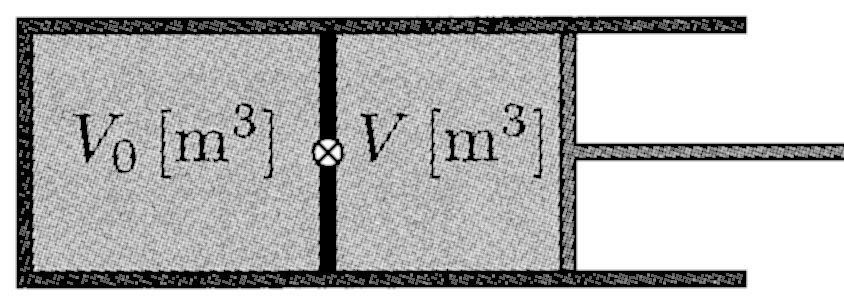
\includegraphics[keepaspectratio,width=54mm]{fig/ch17_a29_3.png}
       \end{center}
       すなわち，この状態変化ではバルブは存在しないのと全く同様にみなせるので，この状態変化は次図と全く同じものとみなせる．
       \begin{center}
       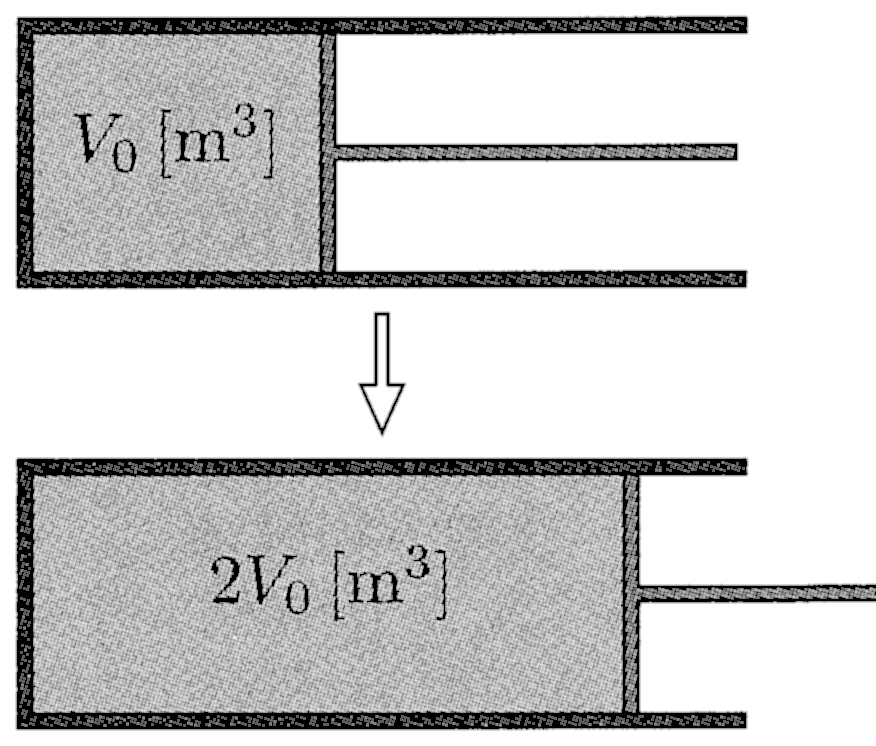
\includegraphics[keepaspectratio,width=52mm]{fig/ch17_a29_4.png}
       \end{center}
       よって，この断熱変化に対してはポアソンの式を適用することができる．この気体の比熱比$\gamma$は
       \[\gamma=\frac{C_P}{C_V}=\frac{C_V+R}{C_V}=1+\frac{R}{C_V}\]
       で与えられるので，終状態の圧力を$p_2\U{Pa}$とすると，ポアソンの式より，
       \[p_0V_0^\gamma=p_2(2V_0)^\gamma\]
       が成立する．これを解いて，
       \[p_2=\frac{1}{2^\gamma}p_0=\frac{1}{2^{1+R/C_V}}p_0\U{Pa}\Ans\]
       また，終状態での温度を$T_2\U{K}$とおくと，状態方程式を立てると，
       \[p_2\cdot 2V_0=nRT_2\]
       よって，
       \[T_2=\frac{1}{2^{R/C_V}}T_0\U{K}\Ans\]
       \begin{bsHosoku}{参考}
       二つの変化それぞれの正しい解法は上述した通りだが，ではなぜ(1)の場合にポアソンの式が利用できないのか？

       それは，(1)の状態変化では，変化途中（すなわち左から右へと気体が拡散している途中）において，気体全体を一つの均一系とみなすことができないからである（23.4 参照）．

       次の図にあるように，気体が左から右へ拡散していく途中では左の気体の方が気体の密度，圧力が高い．そのため，左，右のそれぞれについて状態方程式を立てることはできるが，左＋右をひとくくりにして状態方程式を立てることができない（圧力が共通ではないから）．
       \begin{center}
       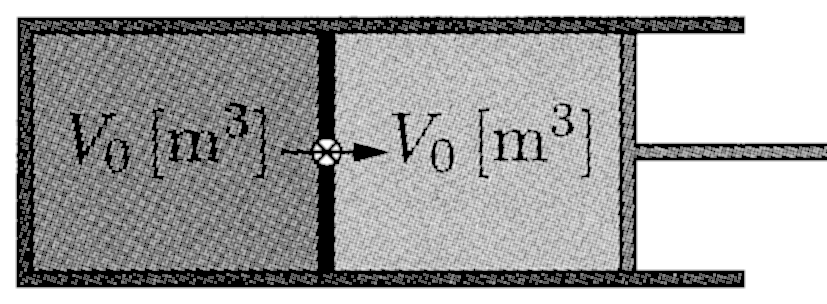
\includegraphics[keepaspectratio,width=54mm]{fig/ch17_a29_ref.png}
       \end{center}
       ポアソンの式の導出では気体全体に対しての状態方程式を利用しているので，(1)のような断熱自由膨張に対してはポアソンの式を利用することができないのである．
       \end{bsHosoku}
\end{komon}

\MonN{30}{状態変化に伴う各物理量の変化}\par\nopagebreak
\begin{sisin}
各状態変化で，熱量，仕事，内部エネルギーのどれが$0$になるのか（もしくは特殊な値・式となるのか）を覚えておき，残りの量については，$-W=\displaystyle\int_{V_{\mathrm{initial}}}^{V_{\mathrm{final}}}P(V)dV$, $\Delta U=nC_V\Delta T$, $Q=\Delta U+(-W)$の各式から正負を判定する．

状態変化前後の状態方程式の両辺を差し引くと，
\[\begin{array}{r@{\;}l}
       & P_1V_1=nRT_1\\
 -)\;\;& P_0V_0=nRT_0\\ \hline
       & P_1V_1-P_0V_0=nR(T_1-T_0)
\end{array}\]
となる．ここで$PV$の項の変化$P_1V_1-P_0V_0$を$\Delta(PV)$と書くと，
\[\Delta(PV)=nR\cdot\Delta T\]
がすべての状態変化に対して成立する．温度変化についてはこれを利用して考えると便利である．
\end{sisin}
\KaiHead
状態変化前を$(P_0,V_0,T_0)$，変化後を$(P_1,V_1,T_1)$とする．$W$は外部が気体に対してした仕事であるから，気体が外部に対してした仕事は$(-W)$で表され，$-W=\displaystyle\int_{V_{\mathrm{initial}}}^{V_{\mathrm{final}}}P(V)dV$が成り立つ．内部エネルギーは絶対温度にのみ依存し$\Delta U=nC_V\Delta T$と表せる．また，熱力学の第一法則より$Q=\Delta U+(-W)$，変化前後の状態方程式を辺々引いて，$P_1V_1-P_0V_0=nR(T_1-T_0)$が成り立つ．体積変化$\Delta V$を$\Delta V=V_1-V_0$とする．
\begin{komon}
\ko{1} 定圧であるから，$-W=P_0\cdot\Delta V$と表せる．\par
       \hspace*{1zw}圧縮しているので$\Delta V<0$であるから$W>0$，また$P_0\cdot\Delta V<0$であるから温度変化は$\Delta T<0$である．よって$\Delta U<0$となり，$Q=\Delta U+(-W)<0$である．
       \[\text{\MARU{1}負，\MARU{2}正，\MARU{3}負，\MARU{4}下降する}\Ans\]
\ko{2} 定積であるから$\Delta V=0$であり，$W=0$である．\par
       \hspace*{1zw}減圧していくので，$P_1V_0-P_0V_0<0$であるから温度変化は$\Delta T<0$である．よって$\Delta U<0$となり，$Q=\Delta U+(-W)<0$である．以上より，
       \[\text{\MARU{1}負，\MARU{2}$0$，\MARU{3}負，\MARU{4}下降する}\Ans\]
\ko{3} 定温であるから温度が一定であり，$\Delta U=0$である．\par
       \hspace*{1zw}加圧しているので$P_1>P_0$であり，状態方程式$P_1V_1=nRT_0$および$P_0V_0=nRT_0$より$V_1<V_0$, すなわち体積は減少している．よって$W>0$であり，$Q=\Delta U+(-W)<0$である．以上より，
       \[\text{\MARU{1}負，\MARU{2}正，\MARU{3}$0$，\MARU{4}一定である}\Ans\]
       \begin{chuu}
       気体が外部にした仕事$(-W)$の正負は$p$-$V$図から考えれば明らかである．定温曲線は次図のように双曲線となるのだから，加圧すれば体積は減少する．よって，$-W<0$となるのはこの図より明らか．
       % 誤植訂正（2026-09-02，旧 physics_ch17.tex から引き継ぎ）：原本は「よって，W<0 となるのは…」．
       \begin{center}
       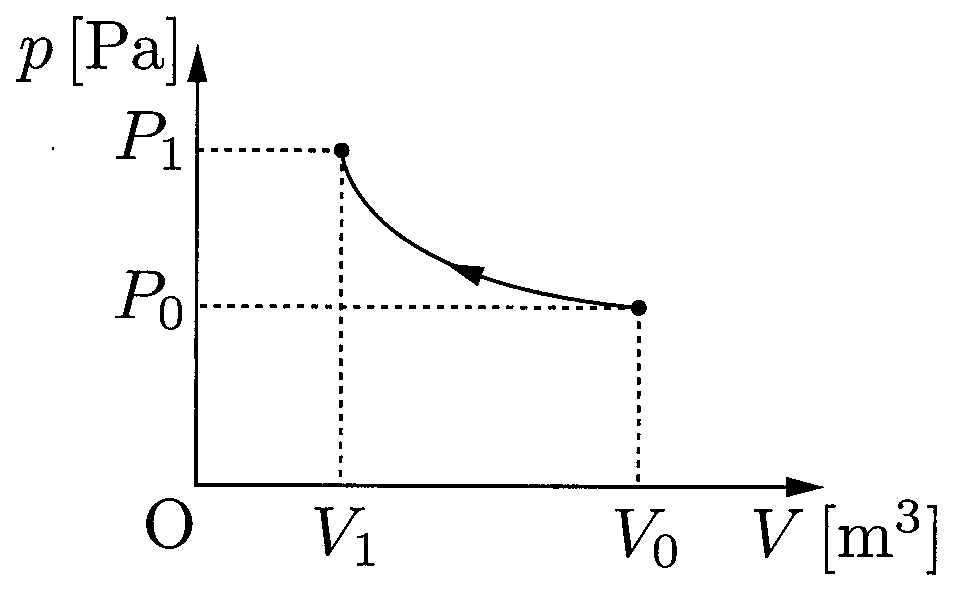
\includegraphics[keepaspectratio,width=54mm]{fig/ch17_a25_pv.png}
       \end{center}
       \end{chuu}
\ko{4} 断熱変化であるから，$Q=0$である．\par
       \hspace*{1zw}圧縮しているので$\Delta V<0$であるから$W>0$，また$\Delta U=Q+W$より$\Delta U>0$であるから温度変化は$\Delta T>0$である．以上より，
       \[\text{\MARU{1}$0$，\MARU{2}正，\MARU{3}正，\MARU{4}上昇する}\Ans\]
       \begin{chuu}
       (1)〜(4)の各状態変化ごとに本質的に覚えておくべきことは最初の一行のみである．あとは指針で述べた関係式から他の物理量の変化が分かる．
       \end{chuu}
\end{komon}

\MonN{31}{サイクル（循環過程）}\par\nopagebreak
\begin{sisin}
熱サイクルの問題では，まず$\mathrm{A}\sim\mathrm{D}$の各状態についての状態方程式を立てておくとよい．$\mathrm{B}\rightarrow\mathrm{C}$と$\mathrm{D}\rightarrow\mathrm{A}$は定圧変化，$\mathrm{A}\rightarrow\mathrm{B}$と$\mathrm{C}\rightarrow\mathrm{D}$は定積変化であり，このときの熱・仕事のやり取りの求め方はすでに分かっているはず．あとはひたすら計算しよう．

(3)では，気体が外界にした正味の仕事$W_{\mathrm{total}}\U{J}$，すなわち外界に対してなした仕事から外界からなされた仕事を差し引いたものが求められており，また外界からもらった熱量$Q_{\mathrm{in}}\U{J}$については，外界からもらった熱のみが聞かれており，外界に対して捨てた熱量は含めないとある．つまり，仕事・熱のやり取りについて，それが外界から受けたものか，外界に与えたものかを判別しなければならない．
\end{sisin}
\KaiHead
\begin{komon}
\ko{1} この気体のモル数を$n\U{mol}$として，$\mathrm{A}\sim\mathrm{D}$の状態に対して状態方程式を立てると，
       \[\begin{aligned}
         \mathrm{A}&:p_0V_0=nRT_0\\
         \mathrm{B}&:(2p_0)V_0=nRT_{\mathrm{B}}\\
         \mathrm{C}&:(2p_0)(3V_0)=nRT_{\mathrm{C}}\\
         \mathrm{D}&:p_0(3V_0)=nRT_{\mathrm{D}}
       \end{aligned}\]
       以上を解いて，
       \[T_{\mathrm{B}}=2T_0\U{K},\ T_{\mathrm{C}}=6T_0\U{K},\]
       \[T_{\mathrm{D}}=3T_0\U{K}\Ans\]
\ko{2} $\mathrm{A}\rightarrow\mathrm{B}$, $\mathrm{C}\rightarrow\mathrm{D}$の二つの状態変化は定積変化であるから，$T$-$V$図でも$T$軸に平行な直線になる．\par
       \hspace*{1zw}$\mathrm{B}\rightarrow\mathrm{C}$では圧力が$p=2p_0$で一定の変化であるから，途中の体積が$V\U{m^3}$のときの温度を$T(V)\U{K}$とすると，状態方程式は
       \[2p_0\cdot V=nR\cdot T(V)\]
       これを解くと，
       \[T(V)=\frac{2p_0}{nR}V=\frac{2T_0}{V_0}V\U{K}\]
       よって，体積$V$に対して温度は一次関数的に変化する．同様に，$\mathrm{D}\rightarrow\mathrm{A}$では圧力が$p=p_0$で一定の変化であるから，
       \[T(V)=\frac{p_0}{nR}V=\frac{T_0}{V_0}V\U{K}\]
       以上をグラフ化して次図の状態変化図を得る．
       \begin{center}
       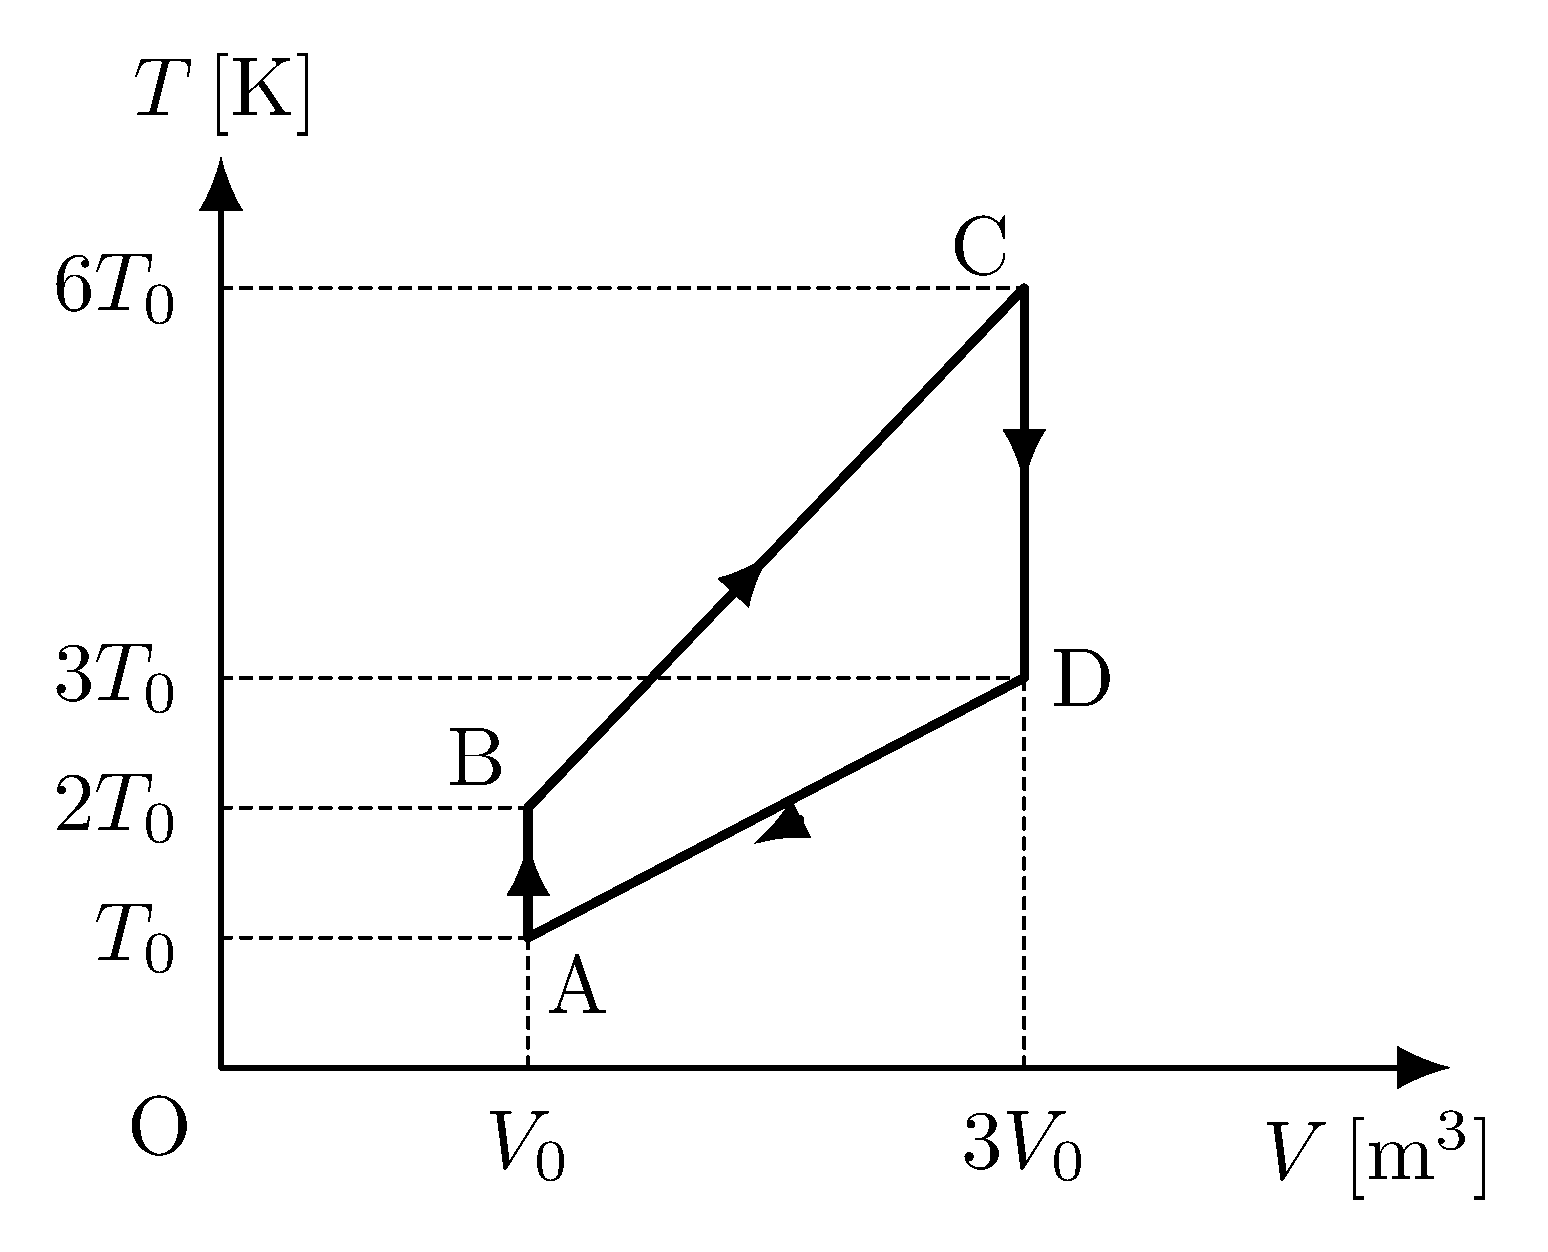
\includegraphics[keepaspectratio,width=60mm]{fig/n23_a31_tv.png}
       \end{center}
       \hspace*{\fill}\Ans
\ko{3} 各状態変化での気体が外界に対してした仕事を$w_1\sim w_4\U{J}$，内部エネルギー変化を$\Delta U_1\sim\Delta U_4\U{J}$，外部が気体に与えた熱量を$Q_1\sim Q_4\U{J}$とする．$\mathrm{B}\rightarrow\mathrm{C}$, $\mathrm{D}\rightarrow\mathrm{A}$が定圧変化であることに注意して
       \begin{list}{}{\setlength{\leftmargin}{1.2zw}\setlength{\itemsep}{0.3mm}\setlength{\topsep}{0.8mm}\setlength{\parsep}{0pt}}
       \item[・] $\mathrm{A}\rightarrow\mathrm{B}$
       \end{list}
       \[w_1=0\U{J}\]
       \[\Delta U_1=nC_V(T_{\mathrm{B}}-T_0)=\frac{C_V}{R}p_0V_0\U{J}\]
       \[Q_1=\Delta U_1+w_1=\frac{C_V}{R}p_0V_0\U{J}\]
       \begin{list}{}{\setlength{\leftmargin}{1.2zw}\setlength{\itemsep}{0.3mm}\setlength{\topsep}{0.8mm}\setlength{\parsep}{0pt}}
       \item[・] $\mathrm{B}\rightarrow\mathrm{C}$
       \end{list}
       \[w_2=2p_0\cdot\Delta V=4p_0V_0\U{J}\]
       \[\Delta U_2=nC_V(T_{\mathrm{C}}-T_{\mathrm{B}})=\frac{C_V}{R}4p_0V_0\U{J}\]
       \[Q_2=\Delta U_2+w_2=\frac{C_V+R}{R}4p_0V_0\U{J}\]
       \begin{list}{}{\setlength{\leftmargin}{1.2zw}\setlength{\itemsep}{0.3mm}\setlength{\topsep}{0.8mm}\setlength{\parsep}{0pt}}
       \item[・] $\mathrm{C}\rightarrow\mathrm{D}$
       \end{list}
       \[w_3=0\U{J}\]
       \[\Delta U_3=nC_V(T_{\mathrm{D}}-T_{\mathrm{C}})=-\frac{C_V}{R}3p_0V_0\U{J}\]
       \[Q_3=\Delta U_3+w_3=-\frac{C_V}{R}3p_0V_0\U{J}\]
       \begin{list}{}{\setlength{\leftmargin}{1.2zw}\setlength{\itemsep}{0.3mm}\setlength{\topsep}{0.8mm}\setlength{\parsep}{0pt}}
       \item[・] $\mathrm{D}\rightarrow\mathrm{A}$
       \end{list}
       \[w_4=p_0\cdot\Delta V=p_0(V_0-3V_0)=-2p_0V_0\U{J}\]
       \[\Delta U_4=nC_V(T_0-T_{\mathrm{D}})=-\frac{C_V}{R}2p_0V_0\U{J}\]
       % 誤植訂正（2026-09-21）：原本は $\Delta U_4=nC_V(T_0-T_{\mathrm{C}})$．
       %   D→A の変化なので $T_{\mathrm{D}}$ が正しい（原本の答の値も $T_{\mathrm{D}}$ で計算されている）．
       \[Q_4=\Delta U_4+w_4=-\frac{C_V+R}{R}2p_0V_0\U{J}\]
       以上より，気体が外界に対してした正味の仕事は，
       \[\begin{aligned}
         W_{\mathrm{total}}&=w_1+w_2+w_3+w_4\\
          &=0+4p_0V_0+0+(-2p_0V_0)\\
          &=2p_0V_0\U{J}\Ans
       \end{aligned}\]
       また，$Q_3$, $Q_4$は負値であり，$\mathrm{C}\rightarrow\mathrm{D}$および$\mathrm{D}\rightarrow\mathrm{A}$の過程では外界に熱を捨てているので，外界からもらった熱量$Q_{\mathrm{in}}$には含まれない．すなわち，外界から熱をもらっているのは$\mathrm{A}\rightarrow\mathrm{B}$および$\mathrm{B}\rightarrow\mathrm{C}$の二つの過程であり，
       \[\begin{aligned}
         Q_{\mathrm{in}}&=Q_1+Q_2\\
          &=\frac{5C_V+4R}{R}p_0V_0\U{J}\Ans
       \end{aligned}\]
       \begin{chuu}
       % 加筆（2026-09-21）：23.5 のまとめ枠の「表にまとめるとよい」の実例．
       %   検算（ΔUの総和が0）もここで示す．
       以上を表にまとめると次のようになる（数値はすべて$p_0V_0$倍したもの）．
       \begin{center}\small
       \begin{tabular}{@{}l@{\hspace{2.5mm}}r@{\hspace{2.5mm}}c@{\hspace{2.5mm}}c@{}}
       過程 & $w$ & $\Delta U$ & $Q$\\ \hline
       $\mathrm{A}\rightarrow\mathrm{B}$ & $0$  & $C_V/R$    & $C_V/R$\\
       $\mathrm{B}\rightarrow\mathrm{C}$ & $4$  & $4C_V/R$   & $4(C_V\!+\!R)/R$\\
       $\mathrm{C}\rightarrow\mathrm{D}$ & $0$  & $-3C_V/R$  & $-3C_V/R$\\
       $\mathrm{D}\rightarrow\mathrm{A}$ & $-2$ & $-2C_V/R$  & $-2(C_V\!+\!R)/R$\\ \hline
       合計 & $2$ & $0$ & \\
       \end{tabular}
       \end{center}
       1周すると元の状態に戻るので，$\Delta U$の列の合計が$0$になっていなければならない．これが計算の検算になる．
       \end{chuu}
       \begin{bsHosoku}{参考}
       本問のように一周して元に戻ってくる場合に関しては，$W_{\mathrm{total}}$は$p$-$V$図上で状態変化曲線が\underline{右回りに}\hskip0pt\underline{囲む面積}になる．例えば本問の場合，$w_2$および$(-w_4)$は次図のような面積（$>0$）として表されるから，差し引いたものは$\mathrm{ABCD}$の循環過程が右回りに囲んでいる面積となる．
       \begin{center}
       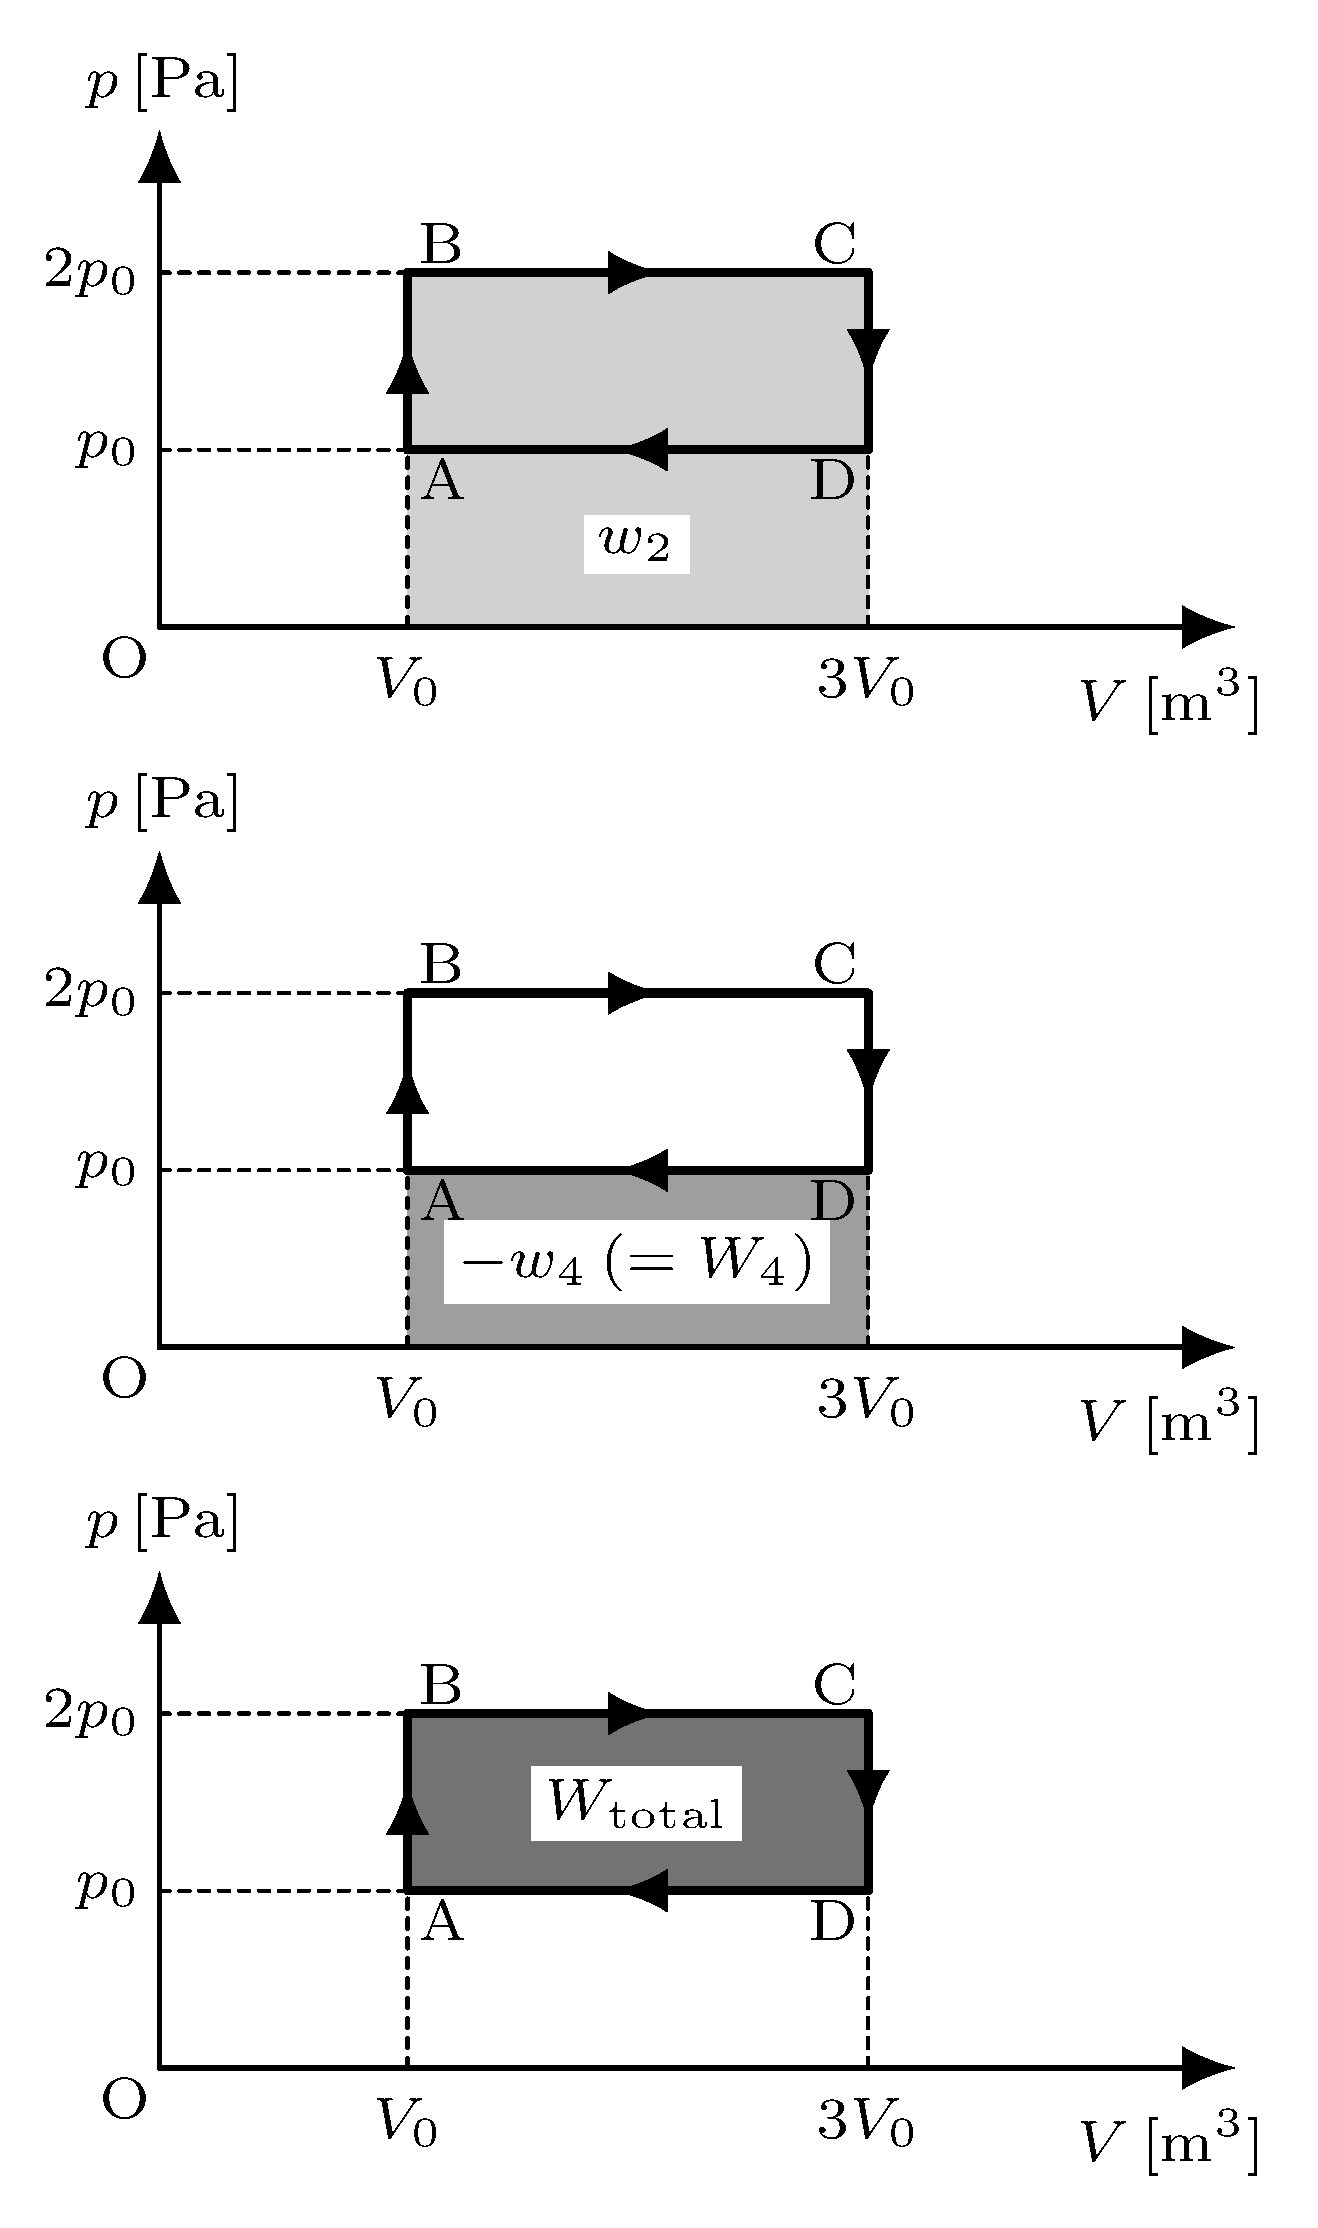
\includegraphics[keepaspectratio,width=62mm]{fig/n23_a31_area.png}
       \end{center}
       \end{bsHosoku}
\ko{4} (3)の答より，
       \[\eta=\frac{W_{\mathrm{total}}}{Q_{\mathrm{in}}}=\frac{2R}{5C_V+4R}\Ans\]
       \begin{bekkai}
       低熱源に捨てた熱量$q$は，$\mathrm{C}\rightarrow\mathrm{D}$と$\mathrm{D}\rightarrow\mathrm{A}$の放熱量の和であるから，
       \[q=-(Q_3+Q_4)=\frac{5C_V+2R}{R}p_0V_0\U{J}\]
       % 誤植訂正（2026-09-21）：原本は右辺が $P_0V_0$（大文字）．本問に $P_0$ は登場しない．
       である．よって 23.5 の式より，
       \[\begin{aligned}
         \eta&=1-\frac{q}{Q_{\mathrm{in}}}=1-\frac{5C_V+2R}{5C_V+4R}\\
             &=\frac{2R}{5C_V+4R}\Ans
       \end{aligned}\]
       としてもよい．
       \end{bekkai}
\end{komon}

\MonN[\Sitei]{32}{サイクル（循環過程）}\par\nopagebreak
\begin{sisin}
基本的な解き方は前問と全く同じである．(1)ではとりあえず外部が気体に与える熱量を求め，その正負を考える．

前問と違い$\mathrm{B}\rightarrow\mathrm{C}$が等温変化なので，この過程の仕事は$w=p\Delta V$では求まらず，23.2 の$w=nRT\log_e\dfrac{V_2}{V_1}$を用いることになる．
\end{sisin}
\KaiHead
\begin{komon}
\ko{1} 気体の物質量を$n\U{mol}$とする．\par
       \hspace*{1zw}$\mathrm{B}\rightarrow\mathrm{C}$の過程は定温過程であり，この温度を$T_1\U{K}$とすると，$\mathrm{A}$, $\mathrm{B}$, $\mathrm{C}$点の状態方程式は
       \[\begin{aligned}
         \mathrm{A}&:p_0V_0=nRT_0\\
         \mathrm{B}&:(2p_0)V_0=nRT_1\\
         \mathrm{C}&:p_0\cdot 2V_0=nRT_1
       \end{aligned}\]
       以上を解いて，
       \[T_1=2T_0\U{K}\]
       各状態変化での気体が外界に対してした仕事を$w_1\sim w_3\U{J}$，内部エネルギー変化量を$\Delta U_1\sim\Delta U_3\U{J}$，外部が気体に与えた熱量を$Q_1\sim Q_3\U{J}$とする．
       \begin{list}{}{\setlength{\leftmargin}{1.2zw}\setlength{\itemsep}{0.3mm}\setlength{\topsep}{0.8mm}\setlength{\parsep}{0pt}}
       \item[・] $\mathrm{A}\rightarrow\mathrm{B}$
       \end{list}
       定積なので，$w_1=0\U{J}$．内部エネルギーは絶対温度に比例するので，
       \[\Delta U_1=nC_V(T_1-T_0)=\frac{C_V}{R}p_0V_0\U{J}\]
       熱力学第一法則$Q_1=\Delta U_1+w_1$より，
       \[Q_1=\frac{C_V}{R}p_0V_0\U{J}\]
       \begin{list}{}{\setlength{\leftmargin}{1.2zw}\setlength{\itemsep}{0.3mm}\setlength{\topsep}{0.8mm}\setlength{\parsep}{0pt}}
       \item[・] $\mathrm{B}\rightarrow\mathrm{C}$
       \end{list}
       変化途中の体積$V\U{m^3}$のときの圧力$P(V)$は状態方程式$P(V)\cdot V=nRT_1$より
       \[P(V)=\frac{2p_0V_0}{V}\U{Pa}\]
       と表せる．これより，
       \[\begin{aligned}
         w_2&=\int_{V_0}^{2V_0}P(V)dV=2p_0V_0\int_{V_0}^{2V_0}\frac{1}{V}dV\\
            &=2p_0V_0\log_e 2\U{J}
       \end{aligned}\]
       $\mathrm{A}\rightarrow\mathrm{B}$のときと同様に考えて
       \[\Delta U_2=nC_V(T_1-T_1)=0\U{J}\]
       \[Q_2=\Delta U_2+w_2=2p_0V_0\log_e 2\U{J}\]
       \begin{list}{}{\setlength{\leftmargin}{1.2zw}\setlength{\itemsep}{0.3mm}\setlength{\topsep}{0.8mm}\setlength{\parsep}{0pt}}
       \item[・] $\mathrm{C}\rightarrow\mathrm{A}$
       \end{list}
       圧力が$p_0$のまま一定なので，
       \[w_3=\int_{2V_0}^{V_0}p_0dV=-p_0V_0\U{J}\]
       $\mathrm{A}\rightarrow\mathrm{B}$のときと同様に考えて
       \[\Delta U_3=nC_V(T_0-T_1)=-\frac{C_V}{R}p_0V_0\U{J}\]
       \[Q_3=\Delta U_3+w_3=-\frac{C_V+R}{R}p_0V_0\U{J}\]
       以上で求めた熱量の正負を見ると，
       \[Q_1>0,\ Q_2>0,\ Q_3<0\]
       であるから，
       \[\text{吸熱過程：}\mathrm{A}\rightarrow\mathrm{B},\ \mathrm{B}\rightarrow\mathrm{C}\text{の二つ}\]
       \[\text{放熱過程：}\mathrm{C}\rightarrow\mathrm{A}\Ans\]
\ko{2} 気体が外界にした正味の仕事$w_{\mathrm{total}}\U{J}$は，$w_1\sim w_3$の総和を考えて，
       \[\begin{aligned}
         w_{\mathrm{total}}&=w_1+w_2+w_3\\
          &=p_0V_0(2\log_e 2-1)\U{J}\Ans
       \end{aligned}\]
       また外界が気体に与えた熱量は，$\mathrm{A}\rightarrow\mathrm{B}$, $\mathrm{B}\rightarrow\mathrm{C}$の二つが正値であるから，
       \[\begin{aligned}
         Q&=Q_1+Q_2\\
          &=\left(\frac{C_V}{R}+2\log_e 2\right)p_0V_0\U{J}\Ans
       \end{aligned}\]
       以上より，この循環過程の熱効率は
       \[\eta=\frac{w_{\mathrm{total}}}{Q}=\frac{(2\log_e 2-1)R}{C_V+(2\log_e 2)R}\Ans\]
       \begin{chuu}
       % 加筆（2026-09-21）：原本は［32］に図が無かった．吸熱・放熱の過程と，
       %   w_total が囲む面積であることを目で確かめられるようにした．
       この過程を$p$-$V$図で見ると次図の通りで，$w_{\mathrm{total}}$はサイクルが右回りに囲む面積である．
       \begin{center}
       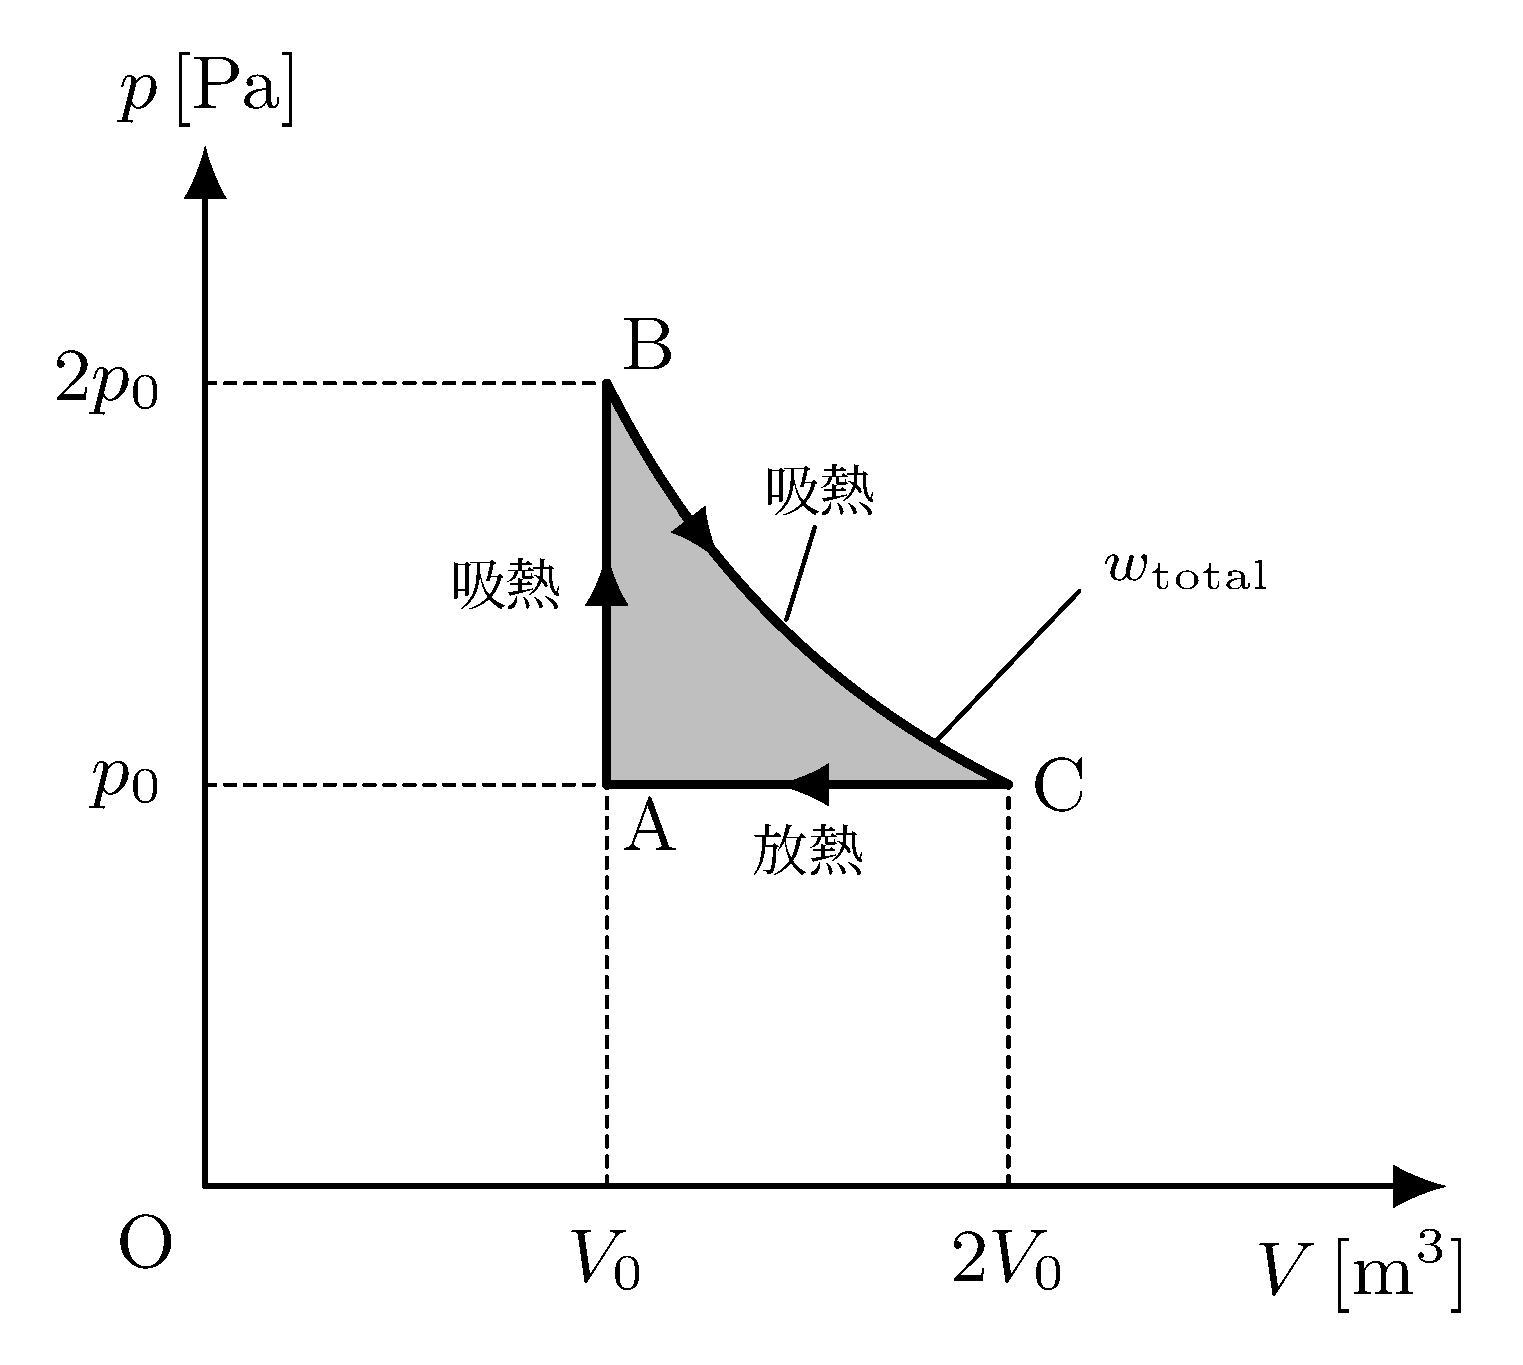
\includegraphics[keepaspectratio,width=62mm]{fig/n23_a32_pv.png}
       \end{center}
       $2\log_e 2-1\fallingdotseq 0.386>0$であり，たしかに正の仕事をしている．
       \end{chuu}
\end{komon}
\begin{bekkai}
$\mathrm{A}\rightarrow\mathrm{B}\rightarrow\mathrm{C}\rightarrow\mathrm{A}$の1サイクル全体について考えると，内部エネルギー変化は
\[\Delta U=0\]
である．この1サイクルで外界に放出した熱量$q$は$\mathrm{C}\rightarrow\mathrm{A}$の過程の放熱量であるから，
\[q=-Q_3=\frac{C_V+R}{R}p_0V_0\U{J}\]
である．1サイクル全体に対する熱力学第一法則を用いて，
\[0=(Q-q)-w_{\mathrm{total}}\]
% 誤植訂正（2026-09-21）：原本は $0=(Q-q)+w_{\mathrm{total}}$ だが，これでは
%   直後の $w_{\mathrm{total}}=Q-q$ と符号が合わない．
が成立するので，
\[w_{\mathrm{total}}=Q-q=(2\log_e 2-1)p_0V_0\U{J}\]
である．また，熱効率については，
\[\begin{aligned}
  \eta&=\frac{w_{\mathrm{total}}}{Q}=1-\frac{q}{Q}\\
      &=1-\frac{C_V+R}{C_V+(2\log_e 2)R}\\
      &=\frac{(2\log_e 2-1)R}{C_V+(2\log_e 2)R}\Ans
\end{aligned}\]
としてもよい．
\end{bekkai}
\begin{bsHosoku}{参考}
最後で求めた熱効率$\eta$（イータと読む）の意味については 23.5 で述べた通りである．熱効率を求める際には本問の(1)のように，やり取りされる熱量について「外部が気体へ与える」のか「気体が外部へ捨てる」のかを判断し，{\gtfamily 与えられた熱量だけ}を分母に数えねばならない．これに対し，仕事は気体が外部に仕事をするときを正として考え，すべて足してしまえば正味の仕事が割り出せる．
\end{bsHosoku}

\Rank{C問題}
\MonN{33}{気体の一般的な状態変化}\par\nopagebreak
\begin{sisin}
本問はバネがあるため，気体の状態変化は定積，定圧，定温，断熱のいずれにも当てはまらない．このような場合には，全ての状態変化に対して成立する次の基本的な流れに従って考えよ．
\begin{list}{}{\setlength{\leftmargin}{1.6zw}\setlength{\itemsep}{0.3mm}\setlength{\topsep}{0.6mm}\setlength{\parsep}{0pt}}
\item[\MARU{1}] $w=\displaystyle\int_{V_{\mathrm{start}}}^{V_{\mathrm{end}}}P(V)dV$の計算
\item[\MARU{2}] $\Delta U=nC_V\Delta T$の計算
\item[\MARU{3}] 熱力学第一法則$Q=\Delta U+w$の立式
\end{list}

なお本問の装置は【例題10】と同じものであり，(2)の$w$は例題10(4)で求めたものと同じである．
% 加筆（2026-09-21）：原本の例題8（本書の例題10）と本問は同一の装置・同一の変化で，
%   例題が (1)〜(4) で仕事までを，本問が温度と熱量までを問う関係にある．
%   両方を残したので，つながりを明示した．
\end{sisin}
\KaiHead
問題の図にある，バネが距離$x\U{m}$だけ縮んだ途中状態における気体の圧力を$P(x)$とすると，ピストンに対して作用する力のつり合いより，
\[P(x)S=P_0S+kx\]
これより，
\[P(x)=P_0+\frac{kx}{S}\U{Pa}\]
また，このときの体積は
\[V(x)=S(l_0+x)\U{m^3}\]
封入されている気体のモル数を$n\U{mol}$とすると，最初の状態の状態方程式は
\[P_0\cdot Sl_0=nRT_0\]
である．
\begin{komon}
\ko{1} 終状態，すなわち$x=a\U{m}$のときは，
       \[P_1=P(a)=P_0+\frac{ka}{S}\U{Pa}\Ans\]
       であり，このときの気体の状態方程式は
       \[P_1\cdot S(l_0+a)=nRT_1\]
       これと最初の状態の状態方程式を組み合わせて解くと，
       \[T_1=\left(1+\frac{ka}{P_0S}\right)\left(1+\frac{a}{l_0}\right)T_0\U{K}\Ans\]
\ko{2} この状態変化で気体がする仕事は，積分を用いて
       \[w=\int_{Sl_0}^{S(l_0+a)}P(V)dV\]
       で求められる．この式の積分変数を$V$から$x$に変えると，
       \[\frac{dV}{dx}=S\;\Leftrightarrow\;dV=Sdx\]
       \[V=S(l_0+a)\;\Leftrightarrow\;x=a\]
       \[V=Sl_0\;\Leftrightarrow\;x=0\]
       であるから，
       \[\begin{aligned}
         w&=\int_0^a\left(P_0+\frac{kx}{S}\right)Sdx\\
          &=\int_0^a(P_0S+kx)dx\\
          &=P_0Sa+\frac{1}{2}ka^2\U{J}\Ans
       \end{aligned}\]
       \begin{chuu}
       圧力$P$を体積$V$で表してもよい．
       \[P(x)=P_0+\frac{kx}{S}\U{Pa}\]
       \[V(x)=S(l_0+x)\U{m^3}\]
       の2式から$x$を消すと，
       \[P(V)=P_0+\frac{k}{S}\left(\frac{V}{S}-l_0\right)\U{Pa}\]
       が得られる．これをもとに$p$-$V$図を描き，その面積（台形）から仕事を求めることができる（【例題10】(3)(4)）．
       \end{chuu}
\ko{3} この状態変化での内部エネルギーの増加は
       \[\Delta U=nC_V(T_1-T_0)\]
       であり，熱力学第一法則$Q=\Delta U+w$を利用すると，
       \[\begin{aligned}
         Q&=nC_VT_0\left(\frac{ka}{P_0S}+\frac{a}{l_0}+\frac{ka^2}{P_0Sl_0}\right)\\
          &\qquad\qquad\qquad+P_0Sa+\frac{1}{2}ka^2\U{J}\\
          &=\frac{C_V}{R}kal_0+\frac{2C_V+R}{2R}ka^2\\
          &\qquad\qquad\qquad+\frac{C_V+R}{R}P_0Sa\U{J}\Ans
       \end{aligned}\]
\end{komon}

\end{multicols}
